\documentclass[11pt]{report}
\usepackage{amsfonts,amsthm,amsmath}
\usepackage{fullpage}
\usepackage{complexity}
\usepackage{graphicx}
\usepackage{tocloft}
\usepackage{enumerate}
\usepackage{collect}		% for problem sets, exercises collection

\usepackage{xcolor}
\usepackage{color}
\definecolor{delta}{rgb}{0,0.2,0}
\definecolor{gamma}{rgb}{0,0,0.2}
\definecolor{beta}{rgb}{0.2,0,0}
\definecolor{alpha}{rgb}{0.8,0,0}

\usepackage{amssymb}
\usepackage{scribe-book}
\usepackage{algorithm}
\usepackage[noend]{algpseudocode}
\usepackage{todonotes}
\usepackage[linkcolor=blue,colorlinks=true]{hyperref}
\usepackage{hypcap}
\renewcommand{\E}{{\mathbb E}}

\newcounter{todocounter}
\newcommand{\todonum}[2][]{\stepcounter{todocounter}\todo[#1]{\thetodocounter: #2}}
\newcommand{\jsay}[1]{\todonum[inline,color=red!20]{\small JS says: #1}}

% modified exercise enviornment to use with collect  package
\newcounter{excount}
\setcounter{excount}{0}
\theoremstyle{plain}
\newtheorem{ex}            [excount]{Exercise}  
                                               
% for exercises which are problem set questions
\newtheorem{exercise-prob}	[theorem]{Exercise} 
						    

%%%%%%%%%%%%%%%%%%%% Exercise and pset macros (start) %%%%%%%%%%%%%%%%%%%%%%%5
% For problem set back reference.
\def\psetbackref{1}

% For exercise
\definecollection{ex.tmp}
\makeatletter
\newenvironment{exercise}
    {\@nameuse{collect*}{ex.tmp}
		  {\begin{ex}}
		    {\end{ex}}{}{}
    }{\@nameuse{endcollect*}}
\makeatother


%%%%%%%%%%%%%%%%%%%%%%%%%%%%%%%%%%%%%%%%%%%%%%%%%%%%%%%%%%%%%%
% To create a a new pset with pset number n, copy paste the following code
% with XX replaced by n.
%
% 	 \definecollection{psXX.tmp}
%	 \makeatletter
%	 \newenvironment{show-psXX}[1]
%	     {\@nameuse{collect*}{psXX.tmp}
%	         {\ifthenelse{ \equal{\psetbackref}{1} }{\label{prob:#1}}{}} {}
%   	         {\item \label{#1} (See Exercise~\ref{prob:#1})} {}
%	     }{\@nameuse{endcollect*}}
%	 \makeatother
%
%	 \makeatletter
%	 \newenvironment{psXX}
%	     {\@nameuse{collect}{psXX.tmp}
%			{\item}{}
%	     }{\@nameuse{endcollect}}
%	 \makeatother
%
% 


%%% For ps1 
\definecollection{ps1.tmp}
\makeatletter
\newenvironment{show-ps1}[1]
    {\@nameuse{collect*}{ps1.tmp}
	    {\ifthenelse{ \equal{\psetbackref}{1} }{\label{prob:#1}}{}} {}
	    {\item \label{#1} (See Exercise~\ref{prob:#1})} {}
    }{\@nameuse{endcollect*}}
\makeatother

\makeatletter
\newenvironment{ps1}
    {\@nameuse{collect}{ps1.tmp}
		{\item}{}
    }{\@nameuse{endcollect}}
\makeatother

%%% For ps2
\definecollection{ps2.tmp}
\makeatletter
\newenvironment{show-ps2}[1]
    {\@nameuse{collect*}{ps2.tmp}
	    {\ifthenelse{ \equal{\psetbackref}{1} }{\label{prob:#1}}{}} {}
	    {\item \label{#1} (See Exercise~\ref{prob:#1})} {}
    }{\@nameuse{endcollect*}}
\makeatother

\makeatletter
\newenvironment{ps2}
    {\@nameuse{collect}{ps2.tmp}
		{\item}{}
    }{\@nameuse{endcollect}}
\makeatother


%%%%%%%%%%%%%%%%%%%% Exercise and pset macros (end) %%%%%%%%%%%%%%%%%%%%%%%%%5



%%%%%%%%%%%%%%%%%%%%%%%%%%%
% Lecture specific macros % 
\newcommand{\cgi}{{\sf Color-GI}}
\newcommand{\compiso}{{\sf COMPUTE-ISO}}
\newcommand{\gi}{\mathcal{GI}}
\newcommand{\ga}{\mathcal{GA}}
\newcommand{\setstab}{ {\sf SetStab}}
\newcommand{\pointstab}{ {\sf PointStab}}
\newcommand{\groupintr}{ {\sf GroupInter}}

%%%%%%%%%%%%%%%%%%%%%%



%\newcommand{\N}{\mathbb{N}}
% Shows lecture titles and sections. Set 0 to list only chapters.
\setcounter{tocdepth}{2}

\begin{document}
\thispagestyle{empty}

\begin{flushright}
\vspace*{3cm}
\makeatletter 
\vskip 10\p@ 
\hrule height 2pt
\vskip 2\p@
\hrule height 1pt
\vskip 11\p@
{\huge Lecture Notes on}\\[3ex]
{\Huge \textbf{Algorithmic Algebra}} 
\end{flushright}

\makeatletter 
\vskip 10\p@ 
\hrule height 2pt
\vskip 2\p@
\hrule height 1pt
\vskip 60\p@
\makeatother


\begin{flushleft}
{\large Jayalal Sarma\\ 
Department of Computer Science and Engineering\\
IIT Madras, Chennai 600036 \\[2ex]
Draft---\today\ and forever
}
\end{flushleft}

\newpage
\pagenumbering{roman}  % Roman numbering in intro portion.
\input{preface}
\newpage
\listoftodos

\newpage
\listofscribe          % For automatic scribe list generation.

%\newpage
%\listofinstr
\newpage
\tableofcontents

\newpage 
\pagenumbering{arabic}  % Arabic page numbering for lectures.
%\part{Introduction, Motivation and the Language}
\newpage \setcounter{page}{1} 
\Lecture{Jayalal Sarma}{Aug 3, 2015}{1}{Introduction, Motivation and
the Language}{K Dinesh}{$\delta$}{K Dinesh}

\section{Overview of the course. Administrative, Academic policies}
\newpage

\section{Introduction and Motivation}
Main theme of this course is to use algebra to solve computational problems.
Let us consider the following two problems :
\begin{description}
	\item [Plagiarism check]
	Given two $C$ programs $P_1$ and $P_2$, check if they are the same
	under renaming of variables.
	\item [Molecule detection]
	Given two chemical molecules check if they have the same structure.
\end{description}

Consider the following simpler variant of plagiarism checking where the program
submitted has just its variables renamed and all other portions of the program
are the same. In this case, given the two versions of the program, we need to
check if there is a way to rename the variables of one program to get the
other one. 

In the second case one could view the given molecules as graphs. The problem
is again similar problem, where we want to see if there is way to rename the
vertex labels of the graph so that under the relabelling both the graphs are
the same.

Our aim in both cases is to check whether the two structures are same under
renaming. We are interested in solving this problem on graphs.

\begin{definition}[Graph Isomorphism]
	Two graphs $X_1(V_1,E_1)$, $X_2(V_2,E_2)$ are said to be isomorphic if
	there is a bijective map $\sigma:V_1 \to V_2$ such that $\forall
	(u,v) \in V_1 \times V_1$, \[(u,v) \in E_1 \iff (\sigma(u), \sigma(v))
	\in E_2 \]
\end{definition}
\begin{problem}
	The \emph{graph isomorphism problem} is the decision problem of
	checking if given two graphs $X_1, X_2$ are isomorphic.
\end{problem}

We are also interested in the following special case of the above problem
called graph automorphism problem. 

\begin{definition}[Graph Automorphism]
	For a graph $X(V,E)$, an automorphism of $X$ is a renaming of the
	vertices of $X$ given by a bijective map $\sigma:V \to V$ such 
	that $\forall
	(u,v) \in V \times V$, \[(u,v) \in E \iff (\sigma(u), \sigma(v))
	\in E \]
\end{definition}
We are interested in the set of all bijections such that they are
automorphisms of $X$. We denote this by $Aut(X)$.
\begin{definition}
	For a graph $X$ on $n$ vertices, 
	$Aut(X) = \{ \sigma ~|~ \sigma :[n] \to [n], \sigma \text{ is an
	automorphism of }X \}$
\end{definition}

Note that an identity map which takes a vertex to itself always belongs to
$Aut(X)$ for all graphs $X$. Hence the question is : are there any bijections
other than the identity map as automorphism of $X$.

\begin{problem}[Graph Automorphism Problem]
	Given a graph $X$ does $Aut(X)$ has any element other than the
	identity element.
\end{problem}

One way to see bijections is via permutations. This is because, every
bijection define a permutation and vice versa.

Let $X$ be an $n$ vertex graph. 
Denote $S_n$ to be the set of all permutations on $n$ elements. Hence $Aut(X)$
can be defined as $\left\{ \sigma ~|~ \sigma \in S_n \text{ and $\sigma$ is an
automorphism of } G\right\}$. 

We now show that the set $Aut(X)$ has some nice properties. Given $\sigma_1,
\sigma_2 \in Aut(X)$, we can compose two permutations as $\sigma_1
\circ \sigma_2 = (\sigma_1(\sigma_2(1)),\sigma_1(\sigma_2(2)), \ldots,  
\sigma_1(\sigma_2(n)))$. This is same as applying $\sigma_2$ on identity
permutation and then applying $\sigma_1$ to the result. We show that
$Aut(X)$ along with the composition operation $\circ$
gives us many nice properties.
\begin{itemize}
	\item If $\sigma_1, \sigma_2 \in Aut(X)$, then $\sigma_1 \circ
		\sigma_2$ is also an automorphism of $X$. The reason is that
		for any $(u,v) \in X \times X$, $(u,v) \in E \iff
		(\sigma_2(u), \sigma_2(v)) \in E$ Now applying $\sigma_1$ on
		the previous tuple, we get that $(\sigma_2(u), \sigma_2(v)) 
		\iff (\sigma_1 \circ \sigma_2(u), \sigma_1 \circ \sigma_2(v))
		\in E$. Hence $(u,v) \in E \iff (\sigma_1 \circ \sigma_2(u),
		\sigma_1 \circ \sigma_2(v)) \in E$.
		This tells that $Aut(X)$ is \emph{closed} under $\circ$.
	\item The composition operation is also \emph{associative}.
	\item \emph{Identity} permutation belongs to $Aut(X)$ as observed
	before.  
	\item Since we are considering bijections, it is natural to
		consider \emph{inverse} for a permutation $\sigma$ denoted
		$\sigma^{-1}$ with the property that $\sigma \circ
		\sigma^{-1}$ is identity permutation. 

\end{itemize}
We gave a definition of inverse for an arbitrary permutation. But then a
natural question is : given $\sigma \in Aut(X)$, is it true that $\sigma^{-1}$
also belongs to $Aut(X)$. It turns out that it is true.
\begin{claim}
	For the graph $X(V,E)$
	$\sigma \in Aut(X) \iff \sigma^{-1} \in Aut(X)$
\end{claim}
\begin{proof}
	Recall that $\sigma \in Aut(G)$ iff $\forall (u,v) \in V \times V$,
	$(u,v) \in E \iff (\sigma(u), \sigma(v)) \in E$. In particular, this
	must be true for $(\sigma^{-1}(u), \sigma^{-1}(v))$ also. This means,
	\[ (\sigma^{-1}(u), \sigma^{-1}(v)) \in E \iff (\sigma(\sigma^{-1}(u)),
	\sigma(\sigma^{-1}(v))) \in E \]
	By definition of $\sigma^{-1}$ we get that 
	$(\sigma^{-1}(u), \sigma^{-1}(v)) \in E \iff (u,v) \in E$. This shows
	that $\sigma^{-1} \in Aut(X)$ 
\end{proof}
Objects which satisfy these kind of properties are called groups.

\section{Overview of the course}
There are two major themes. 
\begin{itemize}
	\item Algorithms for permutation groups.
	\item Algorithms for polynomials.
\end{itemize}

\Lecture{Jayalal Sarma}{Aug 4, 2015}{2}{Algebraic Approach to Primality Testing }{K Dinesh}{$\delta$}{K Dinesh}
In this lecture, we will see an algebraic approach to solving a fundamental
problem in Number Theory.
\section{Application to Number Theory}
Following is an algorithmic question that we are interested.
\begin{problem}
Given a number $n$ in its binary representation, check if it is a prime or not
in time $O(poly(\log N))$.
\end{problem}
\begin{note}
The trivial algorithms that we can think of will depend on $n$ and hence takes
time exponential in its input representation.
\end{note}

Consider the following property about prime number proved by Fermat which is
of interest in this context.
\begin{theorem}[Fermat's Little Theorem] If $N$ is a prime, then $\forall~a, 1
	\le a \le N-1$, \[ a^N = a \mod N \]
\end{theorem}
\begin{proof}
	Fix an $a \in \{1,2,\ldots N-1\}$. Now consider the sequence $a, 2a,
	\ldots, (N-1)a$. The question we ask is : can any two of the numbers
	in this sequence be the same modulo $N$. We claim that this cannot
	happen. We give a proof by contradiction : suppose that there are two
	distinct $r,s$ with $1 \le r < s \le N-1$ and $sa = ra \mod N$. Then
	clearly $N | (s-r)a$ which means $N | a$ or $N | (s-r)$. But both
	cannot happen as $a, s-r$ are strictly smaller than $N$.

	This gives that all the $N$ numbers in our list modulo $N$ are
	distinct. Hence all numbers from $1,2,\ldots, N-1$ appear in the list
	when we go modulo $N$. Taking product of the list and the list modulo
	$N$, we get 
	\[ (N-1)! a^{N-1} = (N-1)! \mod N \]
	By cancelling $(N-1)!$, we get that $a^{N-1} = 1 \mod N$.
\end{proof}
This tells that the above condition is necessary for a number to be prime. If
this test is also sufficient (i.e, if the converse of the above theorem is
true), we have a test for checking primality of a number. But it turns out
that this is not true due to the existence of Carmichael numbers which are not
prime numbers but satisfy the above test.

So one want a necessary and sufficient condition which can be used for
primality testing. For this, we need the notion of polynomials.
\begin{definition}
	A polynomial $p(x) = \sum_{i=0}^d a_ix^i$ with $a_d \ne 0$ denotes a
	polynomial in one variable $x$ of degree $d$. Here $a_i$s are called
	coefficients and each term excluding the coefficient is called a
	monomial. \textbf{A polynomial is said to be identically zero, if all
	the coefficients are zero.}
\end{definition}

A polynomial time algorithm for this problem has been found in 2002 by
Manindra Agarwal, Neeraj Kayal and Nitin Saxena (called as the AKS algorithm). 
In their result, they used the following polynomial characterization for a
prime number.
\begin{theorem}[Polynomial formulation (Agarwal-Biswas 1999)] Let $N \ge 1$ be
	an integer. Define a polynomial 
	$p_N(z) = (1+z)^N - 1 - z^N$. Then \[ p_N(z) \equiv 0 (mod~ N)
	\iff N \text{ is prime} \]
\end{theorem}

Hence checking if $N$ is prime or not boils down to checking if $p_N(z)$ is
identically $0$ or not except for the fact that the underlying operations are
done modulo $N$.

Proof of the theorem is as follows.
\begin{proof}
	Note that $p_N(z) = \sum_{i=1}^{N-1} \binom{N}{i} z^i$ and
	$\binom{N}{i} = \frac{N(N-1)\ldots (N-i+1)}{1\cdot 2 \ldots i}$ with $1
	\le i \le N-1$. 

	If $N$ is prime, then $\binom{N}{i} = N \times k_i$ for some integer
	$k_i$ as none of $1, 2, \ldots i$ divides $N$. Hence $\binom{N}{i}
	\mod N = 0$ for every $i$ and $p_N(z) \equiv 0 \mod N$ since the
	polynomial has all coefficients as zero.

	If $N$ is composite, we need to show that $p_N(z) \not 
	\equiv 0 (mod~ N)$ which means that there is at least one non-zero
	coefficient $p_N(z) \mod N$\footnote{In class we asked the following
		question of finding an $a \in \{1,2,\ldots, N-1\}$ such that
	$p_N(a) \ne 0 \mod N$. This has a counter example. Consider the case
	where $N$ is a Carmichael number. By definition, Carmichael numbers
	are composite numbers that satisfy Fermat's Little theorem.  Hence if
	$N$ is Carmichael,  $\forall~ a \in \{1,2,\ldots N-1 \}$, we get  $a^N
	= a \mod N$. This gives that $\forall~ a \in \{1,2,\ldots, N-1\}$
	\[	p_N(a)  = ((a+1)^N-a^N -1) \mod N = ((a+1)-a-1) \mod N \]
	which is zero modulo $N$.}. 	
	Since $N$ is composite, there exists a prime $p$ such that $p
	~|~ N$.  Let $p^k | N$ where $k \ge 1$ is the largest exponent of $p$
	in the prime factorization of $n$. Hence $p^{k+1} \nmid N$.
	
	We first show that $p_N(z)$ is a non zero polynomial by showing that
	the coefficient of $z^i$ for $i = p$, which is $\binom{N}{p}$, is non
	zero modulo $p^k$ showing\footnote{Note that if
		$N|\binom{N}{i}$ then $p^k | \binom{N}{i}$. Taking
		contrapositive, we get that $\binom{N}{i} \not = 0 \mod p^k$
		implies $\binom{N}{i} \not = 0 \mod N$} $p_N(z)$ is not a zero
		polynomial modulo $N$. 
	Let $N = g \times p^k$. In $\binom{N}{p}$, $p$ of the denominator 
	divides $N$. Note that $p$ cannot divide $g$, for if it does, then
	$p^{k+1} | N$ which is not possible by choice of $p$ and $k$.
		\begin{equation}
		\binom{N}{p} = \frac{g\times p^k(N-1)\ldots (N-p+1)}
		{1\cdot 2 \ldots p} = \frac{g\times p^{k-1}(N-1)\ldots 
			\label{eq:ag-bis-proof}
		(N-p+1)}{1\cdot 2 \ldots p-1} \end{equation}
	Hence it must be that $p^{k-1}$ divides $\binom{N}{p}$. This is
	because, there is no $p$ left now in the denominator to divide $N$.
	Now $p^k \nmid \binom{N}{p}$ because, none of the terms $(N-1),
	\ldots,
	(N-p+1)$ can have $p$ as a factor since all these terms are obtained by
	subtracting at most $p-1$ times from $N$. Hence $\binom{N}{p} \ne 0
	\mod p^k$. This completes the proof.
\end{proof}

Note that Fermat's Little Theorem is a special case of Agarwal-Biswas
formulation of primality testing.
\begin{claim}
Fermat's Little Theorem is a special case of Agarwal-Biswas theorem.
\end{claim}
\begin{proof}
	To prove Fermat's Little theorem, we need one direction of implication
	of Agarwal-Biswas theorem : 
	\begin{center}
	``If $N$ is prime, then $(1+z)^N = (1+z^N) \mod N$''.
	\end{center}

	Note that Fermat's Little theorem asks about $a^N \mod N$ for $a \in
	\{1,2,\ldots,N-1\}$. Since the implication talks about $z^N \mod N$
	and $(1+z)^N \mod N$, this suggests an induction strategy on $a$.

	Let $N$ be prime. We check the base case : for $a=1$, the
	$1^N =1 \mod N$. Hence the base case is true. By induction, suppose
	that $a^N = a \mod N$ for $a \in \{1,2,\ldots, N-1\}$. Now, 
	\begin{align*}
		(a+1)^N & = (a^N +1) \mod N && [\text{By Agarwal-Biswas as $N$
		is prime}]\\
		& = (a+1) \mod N && [\text{By inductive hypothesis}]
	\end{align*}
	This completes the inductive case. 
\end{proof}

This shows that checking if the polynomial $p_N(z)$ is a zero polynomial is an if and only if check for primality of $N$. 
So checking primality of a number now boils down to checking if a polynomial is identically zero or not. This is a fundamental problem of polynomial identity testing. We will be discussing about polynomial identity testing and AKS algorithm in our next theme.

\begin{remark}
One could consider two possible definitions of a polynomial being identically zero and they are not equivalent. Indeed, if all coefficients of a polynomial are zeros then it evaluates to zero on all substitutions of the variables. However, the converse need not be true in all underlying algebraic structures. For example, consider the polynomials $x^p -  x$ in a field $\Z_p$ (operations are $+$ and $\times$ modulo $p$). This is indeed a non-zero polynomial but all evaluations modulo $p$ are zero.
\end{remark}

\Lecture{Jayalal Sarma}{Aug 5, 2015}{3}{Algebraic Approach to finding Perfect Matchings in Graphs}{K Dinesh}{$\delta$}{K Dinesh}
\noindent

\section{Application to Graph algorithms}
Consider the following problem of finding perfect matching.
\begin{definition}[Finding Perfect Matching]
Given a bipartite graph $G(V_1,V_2, E)$, we need to come up with an $E'
\subseteq E$ such that $\forall u \in V_1 \cup V_2$, there is exactly one edge
incident to it in $E'$.
\end{definition}

We shall give a polynomial formulation for the problem. Given $G(V_1, V_2, E)$
with vertex sets $|V_1| = |V_2| = n$. Define an $n\times n$ matrix $A$ where
$A(i,j) = 1$ if $(i,j) \in E$ and is $0$ otherwise for all $(i,j) \in V_1 \times
V_2$. Recall the determinant of $A$ given
by
\[ det(A) = \sum_{\sigma \in S_n} sign(\sigma) \prod_{i=1}^n A_{i,\sigma(i)}
\]

where \[
sign(\sigma) = \begin{cases} 
	  -1  & \text{ if } inv(\sigma) \text{ is even} \\
	  1 & \text{ if } inv(\sigma) \text{ is odd}
\end{cases}\]
and $inv(\sigma)$ is defined as 
$\left |\{(i,j) ~|~ i < j \text{ and } \sigma(i) > \sigma(j), 1 \le i<j \le n\}
\right |$.
We denote $f(x) \equiv 0$ to denote that polynomial $f(x)$ is the zero
polynomial.
\begin{lemma}
For the matrix $A$ as defined as before, $det(A) \not \equiv 0 \implies
\text{$G$ has a perfect matching}$ \label{lem:det_pm_simple}
\end{lemma}
\begin{proof}
Let $det(A) \not \equiv 0$. Hence there exists a $\sigma \in
S_n$ such that $\prod_{i=1}^n A_{i, \sigma(i)} \ne 0$. Hence the edge set
$E' = \{(i, \sigma(i)) ~|~ 1\le i\le n\}$ exists in $G$ and since $\sigma(i) =
\sigma(j)$ iff $i=j$ for every $i,j$, $E'$ form a perfect matching.

\end{proof}
Note that converse of this statement is not true. For example, consider the
bipartite graph whose $A$ matrix is $A = 
\begin{bmatrix}
		1 & 1 & 0  \\
		1 & 1 & 0  \\
		0 & 0 & 1  
\end{bmatrix}
$. It can be verified that $det(A) = 0$ but the bipartite graph associated has
a perfect matching.

Hence the next natural question, similar to our primality testing problem, is 
to ask for some kind of modification so that 
converse of previous lemma (lemma~\ref{lem:det_pm_simple}) is true. In the
example considered, there were two perfect matchings in $G$ having opposite 
sign due to which the determinant became $0$. So the modification should
ensure that perfect matchings of opposite signs does not cancel off in the
determinant.

One way to achieve this is as follows.  Define a matrix $T$ as
\[ T(i,j) = \begin{cases}
		x_{ij} & (i, j) \in E \\
		      0 & \text{ otherwise}
	\end{cases}
\]
where $(i,j) \in V_1 \times V_2$. This matrix is called as the Tutte matrix.
Now, if we consider determinant of this matrix, we can see that the monomials
corresponding a $\sigma \in S_n$ can be a product of at most $n$ variables.
Hence $det(T)$ is a polynomial in $n^2$ variables with degree at most $n$.

Also in the expansion of determinant, we can observe that each term picks
exactly one entry from every row and column meaning each of the entries 
picked is from a distinct row and column. Hence each of the them is a
bijection and hence is a permutation on $n$ elements. Also corresponding to any
permutation on $n$ elements, we can get a term. This gives us the following
observation.

\begin{observation}
	Set of monomials in $det(T)$ is in one-one correspondence with set of
	all permutations on $n$.
\end{observation}


% TODO do 3x3 det example.

We now give polynomial formulation for the problem of checking perfect
matching in a bipartite graph.
\begin{claim}
For the matrix $T$ as defined before, $det(T) \not \equiv 0 \iff \text{$G$
has a perfect matching}$
\end{claim}
\begin{proof}
	By $det(T) \equiv 0$, we mean that the polynomial $det(T)$ has all
	coefficients as zero. 
($\Rightarrow$) Since $det(T) \not \equiv 0$, there exists a $\sigma \in S_n$
such that the monomial corresponding is non-zero and by definition of
determinant it must be expressed as product of some $n$ set of variables
$\prod_i T(i,\sigma(i))$. The variable indices gives a matching and since
there are $n$ variables this is a perfect matching.

($\Leftarrow$) Suppose $G$ has a perfect matching given by a $M$. Let $\tau$ 
denote the permutation corresponding to $M$. We now
need to show that $det(T) \not \equiv 0$. To prove this, it suffices to show
that there is a substitution to $det(T)$ which evaluates to a non-zero value. 

Consider the following assignment, $\forall~i,j$ 
\[ a_{ij} = \begin{cases}
		1 & \text{ if } (i,j) \in M \\
		0 & \text{ otherwise}
	\end{cases} 
\]
From the formula of determinant, 
\begin{align*}
	det(T) & = \sum_{\sigma \in S_n} sign(\sigma) \prod_{i=1}^n T_{i,
	\sigma(i)}  \\
	& = sign(\tau)\prod_{i=1}^n A_{i, \tau(i)} + \sum_{\sigma \in S_n
	\setminus \{\tau\}} sign(\sigma)\prod_{i=1}^n T_{i, \sigma(i)}
\end{align*}
Now substituting $x_{ij} = a_{ij}$, we get that the first term evaluates to
$sign(\tau)$ since all the entires are $1$. The second term evaluates to $0$
since for all $\sigma \ne \tau$, there must be a $j$ such that $\sigma(j) \ne
\tau(j)$. Hence it must be that $a_{j, \sigma(j)} = 0$ and hence the product
corresponding to $\sigma$ goes to $0$.
\end{proof}

Hence to check if the bipartite graph $G$ has a perfect matching or not, it
suffices to check if the polynomial $det(T)$ is identically zero or not.
Checking if a polynomial is identically zero or not is one of the fundamental
question in this area.

Note that this problem becomes easy if the polynomial is given as sum of 
monomial form. In most of the cases, the polynomial will not be given this way.
For example if we consider our problem, we are just given the $T$ matrix and
$det(T)$ is the required polynomial. Trying to expand $det(T)$ and simplifying
will involve dealing with $n!$ monomials which is not feasible.

Hence the computational question again boils down to checking if a polynomial
is identically zero or not.
%So far we have spoken about finding perfect matching in bipartite graphs. A
%similar result holds for general graphs also. 
%\begin{theorem}
%Given a graph $G(V,E)$ and for $i, j \in V$, $i \ne j$, define an $n \times n$
%matrix $T$ as
%\[T_{i,j} = \begin{cases}
%		x_{ij} & (i,j) \in E, i < j\\
%	       -x_{ji} & (i,j) \in E, i > j\\
%   	        0 & \text{otherwise}
%	    \end{cases}
%    \]
%	    Then, $det(T) \not \equiv 0 \iff \text{G has a perfect matching}$.
%\end{theorem}



\Lecture{Jayalal Sarma M.N.}{Aug 7, 2015}{4}{Graphs, Groups and
Generators}{Ramya C}{$\delta$}{Ramya C}

In this lecture we will pose three graph theoretic questions and find answers using approaches in algebra.

\section{Graph Isomorphism, Automorphism and Rigidity}

\begin{definition}(Graph Isomorphism.)
Let $G_1=(V_1,E_1)$ and $G_2=(V_2,E_2)$ be graphs. We say $G_1\stackrel{\sim}{=}G_2$ (read as $G_1$ is \em isomorphic to $G_2$) if there exists a bijection $\sigma : V_1\rightarrow V_2$ such that $\forall (u,v) \in V_1\times V_2$ we have

\begin{center}
$(u,v)\in E_1 \iff (\sigma(u),\sigma(v))\in E_2$
\end{center}
\end{definition}

In other words, we say a graph $G_1$ is isomorphic to $G_2$ if there exists a relabeling of the vertices in $G_1$  such that the the adjacency and non-adjacency relationships in $G_2$ is preserved. 
\begin{observation}
If $|V_1|\neq |V_2|$ ,then $G_1$ is not isomorphic to $G_2$.
\end{observation}

The graph isomorphism problem is stated as follows. 

\begin{problem}[{\bf Graph Isomorphism Problem}]
Given two graphs $G_1=(V_1,E_1)$ and $G_2=(V_2,E_2)$, test if $G_1\stackrel{\sim}{=}G_2$ or not.
\end{problem}

A natural question to ask in this setting is that if there is an isomorphism from a graph $G$ to itself. 

Let $[n]=\{1,2,\ldots,n\}$. Let $S_n$ denote the set of all permutations from the set $[n]$ to $[n]$. Let $G=(V,E)$ be a graph. An automorphism of $G$ is a bijection $\sigma:V\rightarrow V$ such that $\sigma(G)= G$. Let
$$Aut(G)= \left\{\sigma | \sigma\in S_n \text{~and~} \sigma(G)= G \right\}$$
be the set of all automorphisms of $G$. Ideally, we would like to compute the set of automorphism of a graph to itself.

\begin{problem}[{\bf Graph Automorphism Problem}]
Given a graph $G$, list the elements of $Aut(G)$.
\end{problem}

The above problem can be expected to be solved in polynomial time only if the output expected is polynomial in length. This brings up the size of the $Aut(G)$ into question. Unfortunately, if $G$ is the complete graph on $n$ vertices. Then $|Aut(G)|=n!$. Hence the above question is not well-formulated.

Since identity permutation is trivially an automorphism for any graph, the $Aut(G)$ is always a non-empty subset of $S_n$ where $n$ is the number of vertices. Hence, one can ask a natural decision variant of the above problem, namely the graph rigidity problem.

Formally, the graph rigidity problem is stated as follows.
\begin{problem}[{\bf Graph Rigidity Problem}]
Given a graph $G$, test if $Aut(G)$ is trivial. That is, whether $Aut(G)$ contains only the identity permutation or not.
\end{problem}

More than the size, in the first lecture of this course, we have seen that $Aut(G)$ forms a \textit{subgroup} of $S_n$. To utilize this structure, we first refresh the definition of an abstract group. From now on, we will use the letter $X$ to denote a graph and $G$ to denote a group. 


\section{Groups and Generators}

\begin{definition}(Groups.)
A set $G$ together with a binary operation $*$ is said to be a group if the following four consitions are met
\begin{itemize}
\item \textbf{Closure} : $a,b\in G$, the element $a*b\in G$.
\item \textbf{Associative} : For any $a,b,c\in G$, we have $(a*b)*c = a*(b*c)$.
\item \textbf{Existence of Identity} : For any $a\in G$ there exists a unique element $e\in G$ such that $a*e =e*a =a$. 
\item \textbf{Existence of Inverse} : For any $a\in G$ there exists a unique element $b\in G$(denoted by $a^{-1}$) such that $a*b =b*a =e$. 
\end{itemize}
\end{definition}

\begin{example}
\begin{itemize}
\item $S_n$ forms a group under composition.
\item $(\mathbb{Z}_5,+)$ is a group.
\end{itemize}
\end{example}


From now on, we will use the letter $X$ to denote a graph and $G$ to denote a group.

\begin{remark} 
Let $(G,*)$ be a group. Let $H\subseteq G$ such that $(H,*)$ also forms a group. We say $H$ is a {\em subgroup} of $G$ and denote by $H\leq G$.   
\end{remark}


\begin{exercise}
For any graph X, the set $Aut(X)$ forms a group under the composition operation. That is, $Aut(G)\leq M$ where $M=(S_n,\circ)$ is the permutation group.
\end{exercise}

Let $(G,*)$ be a group. Let $H\subseteq G$ such that $(H,*)$ also forms a group. We say $H$ is a {\em subgroup} of $G$ and denote by $H\leq G$. We showed in the first lecture of the course that, for any graph X, the set $Aut(X)$ forms a group under the composition operation. That is, $Aut(G)\leq M$ where $M=(S_n,\circ)$ is the symmetric group.


Let $(G,+)$ be a finite group and $g\in G$ be an element. Let $g^2 =  g*g ,g^3 =  g*g*g $. Similarly $g^k = \underbrace{g*g*\cdots * g}_\text{k times}$. Now consider the set $H=  \{g,g^2,g^3,\ldots\}$. Since $(G,*)$ is a finite group there must exist a $k$ such that $g^k=g$ in $H$.

\begin{lemma}
Let $(G,+)$ be a finite group and $g\in G$ be an element. Let $H=\{g,g^2,g^3,\ldots\}$ be a set of elements. The unique identity $e$ of $G$ is in $H$.
\end{lemma}
\begin{proof}
Since $(G,*)$ is a finite group there must exist a $k$ such that $g^k=g$ in $H$. By definition, $g^k = g^{k-1}*g = g$. As $(G,*)$ is a group, $g^{-1}$ exists in $G$.\\
Therefore,
\begin{center}
$g^{k-1}*g*g^{-1} = g*g^{-1} = e$ 
\end{center}
\end{proof}


\begin{definition}[\textbf{Generator}]
Let $(G,+)$ be a finite group and $g\in G$ be an element. We say an element $g\in G$ is a generator of the set $H$ if for every element $h\in H$ there exists a $m$ such that $h=g^m$.  (denoted by $H=\langle g \rangle$).
\end{definition}

\begin{observation}$H = \langle g \rangle$ is a subgroup of $G$. That is, $H\leq G$.
\end{observation}

A quick example is that $1$ is a generator for $(\mathbb{Z}_5,+)$



\begin{definition}
An group $(G,*)$ that can be generated by a single element is called a {\em cyclic group}. For instance, $(\mathbb{Z}_5,+)$.
\end{definition}

Not every group is cyclic. For instance, one can verify that $S_3$ (with 6 elements in it) is not cyclic. 

\begin{definition}[\textbf{Generating Set}]
Let $S\subseteq G$ be the set $\{u_1,\ldots,u_k\}$. $S$ is said to be {\em generating} if $\gen{S} = G$.  
\end{definition}

Having observed that $Aut(X)$ could have potentially be of exponential size, a reasonable way to formulate the graph automorphism problem is in terms of the generating set of the group. For this, we establish first that $Aut(X)$ have a generating set of size $\poly(n)$? In fact any group has !.

\subsection{Lagrange's theorem}

Let $(G,*)$ be a group. Let $H\leq G$. For any $g\in G$, define the right coset of $H$ in $G$ to be
$$Hg= \{hg \mid h\in H \}$$

Let $g_1,g_2\in G$ and $Hg_1,Hg_2$ be the corresponding right cosets.  Are there elements that belong to more than one coset of $H$ in $G$? Is $Hg_1\cap Hg_2 \neq \phi$ ? If yes, then the set of right cosets of $H$ in $G$ form a partition of the ground set of $G$. In that case, how many such cosets are required to cover the entire set $G$ ? Let us answer these two questions.

\begin{lemma}
\label{lag1}
Let $g_1,g_2\in G$ and $Hg_1 = \{hg_1\mid h\in H\},Hg_2 = \{hg_2\mid h\in H\}$. Then 
\begin{center}
$Hg_1=Hg_2$ or $Hg_1\cap Hg_2 = \phi$.
\end{center}
\end{lemma}
\begin{proof}
If $g_1=g_2$, then by definition $Hg_1=Hg_2$. Therefore let $g_1\neq g_2$. We will prove : If $Hg_1\cap Hg_2 \neq \phi$ then $Hg_1 = Hg_2$. Let $Hg_1\cap Hg_2 \neq \phi, g\in Hg_1\cap Hg_2$ we will show 
\begin{itemize}
\item[(i)] $Hg_1\subseteq Hg_2$ ; and
\item[(ii)] $Hg_2\subseteq Hg_1$.
\end{itemize}

Since $g\in Hg_1$ we know that there exists a $h_1\in H$ such that $g=h_1g_1$. Similarly $g\in Hg_2$ suggests that there exists a $h_2\in H$ such that $g=h_2g_2$.
\begin{center}
$h_1g_1=h_2g_2=g$
\end{center}   
As $(H,*)$ is a group by itself, $h_1^{-1}$ and $h_2^{-1}$ exists.
\begin{equation}
\label{eqn1}
g_1= h_1^{-1}h_2g_2
\end{equation}

\begin{equation}
\label{eqn2}
g_2 = h_2^{-1}h_1g_1
\end{equation}

\begin{itemize}
\item[(i)] $Hg_1\subseteq Hg_2$ \\
Let $g'\in Hg_1$. This implies there exists a $h'\in H$ such that $g'=h'g_1$. Therefore,
\begin{align*}
g'&= h'g_1\\
g'&= h'(h_1^{-1}h_2g_2) \hspace*{10mm} [\text{By equation \eqref{eqn1}}]
\end{align*} 
By closure property in $(H,*)$, we have $h''=h'h_1^{-1}h_2\in H$. Therefore $g'=h''g_2$, $g'\in Hg_2$.
\item[(ii)] $Hg_2\subseteq Hg_1$ \\
Let $g'\in Hg_2$. This implies there exists a $h'\in H$ such that $g'=h'g_2$. Therefore,
\begin{align*}
g'&= h'g_2\\
g'&= h'(h_2^{-1}h_1g_1) \hspace*{10mm} [\text{By equation \eqref{eqn2}}]
\end{align*} 
By closure property in $(H,*)$, we have $h''=h'h_2^{-1}h_1\in H$. Therefore $g'=h''g_1$, $g'\in Hg_1$.
\end{itemize}
\end{proof}

\begin{lemma}
\label{lag2}
For every $g\in G$, $|Hg|=|H|$.
\end{lemma}
\begin{proof}
By construction, for every element in $H$ there exists an element in $Hg$. So $|Hg|\leq |H|$. We first argue that $|H|\leq |Hg|$. Suppose not. Let $|Hg|<|H|$. Then there exists $h_1,h_2 \in H, h_1 \neq h_2$ such that $h_1 g = h_2 g$. Since $(G,*)$ is a group, $g^{-1}$ exists. We have $h_1gg^{-1} = h_2gg^{-1}$ which implies $h_1=h_2$, a contradiction.
\end{proof}

\begin{theorem}[\textbf{Lagrange's Theorem}]
\label{lag-thm}
Let $(G,*)$ be a group and $H\leq G$. Then $|H|$ divides $|G|$.
\end{theorem}
\begin{proof}
Direct consequence of Lemmas \ref{lag1} and \ref{lag2}
\end{proof}

\begin{observation}
\label{obs-genset}
Let $H=<g>$ and $H'=<H,g'>$ where $g'\in G\backslash H$. Then $H\leq H'\leq G$. We have $g\in H'\backslash H$, therefore $|H'|>|H|$. $H'\leq H$. By Theorem \ref{lag-thm}, $|H'|\geq 2|H|$. This shows that every group has a generating set of size $\log|G|$.
\end{observation}

\begin{remark}
We know that $Aut(X)\leq S_n$ for any graph $X=(V,E)$. By Observation \ref{obs-genset} $Aut(X)$ has a generating set of size $\log|S_n| = log(n!) \in \mathcal{O}(n\log n)$.
\end{remark}  



\Lecture{Jayalal Sarma}{August, 10 2015}{5}{Orbit-Stabilizer Lemma}{Ameya Panse}{$\delta$}{Ramya C}

We first start with some notations and definitions. Order of a group $G$ is number of elements in the group, that is $|G|$. Let $H \le G$ and $g \in G$. The right coset of $H$ in $G$ is defined as 
$Hg = \{hg \mid h \in H\}$. If the multiplication is on the left, we call it the left coset. That is, $gH = \{gh \mid h \in H\}$. In general, it is not necessary that the left and right cosets are the same.
If $H$ is a group such that left and right cosets are the same element-wise, (that is, $\forall g \in G, Hg= gH$), $H$ is a said to be a normal subgroup of $G$.

Let $H$ be a normal subgroup of $G$. Choose one element from each of these as a representative of the set (say $[g]$ denote the coset representative of the coset $Hg = gH$). These elements have a group structure among them. This requires a proof, which we will come to in the next few lectures.

\section{Group Action and Orbits}

Let $G$ be a Subgroup of $S_n$. Let $\alpha \in [n]$ and $g \in G$. We denote by $\alpha^g$ is the image of $\alpha$ under the permutation $g$. 
Orbit of an element $\alpha$ in $G$ is the set of elements it gets mapped to under permutations in $G$. More formally,

\begin{definition}[\textbf{Orbit of $\alpha$ in $G$}]
The orbit of $\alpha$ in $G$ is defined as
\begin{center}
$\alpha^G = \{\alpha^g \mid g \in G\}$
\end{center}
\end{definition}

This defines a natural relation among elements of $[n]$.
$$\alpha \backsim \beta \leftrightarrow \exists g \in G, \alpha^g = \beta$$

We check that this is an equivalence relation. $e \in G$, where e is the identity element. Hence, $\alpha \backsim \alpha$. Let $\alpha \backsim \beta$. Thus $\exists g \in G, \alpha^g = \beta$. Hence, $\alpha = \beta^{g^{-1}}$. Thus, $\beta \backsim \alpha$. The relation $\backsim$ is an equivalence relation. For transitivity, let $\alpha \backsim \beta, \beta \backsim \gamma$. By definition, $\exists g_1, g_2 \alpha^{g_1} = \beta, \beta^{g_2} = \gamma$. By composition of permutations, $(\alpha^{g_1})^{g_2} = \gamma$. Hence, $\alpha \backsim \gamma$.

The stabilizer of $\alpha$ in $G$ is $$G_{\alpha} = \{g \mid \alpha^g = \alpha\}$$. This is the set of elements in $G$ which sends $\alpha$ to $\alpha$ itself. 

\subsection{Orbit-Stabilizer Lemma}

Is there any connection between the number of permutations in $G$ that fixes $\alpha$ and the number of elements to which $\alpha$ can be taken to? The orbit stabilizer lemma, which is an easy consequences of Lagrange's theorem gives a neat answer.

\begin{lemma}[\textbf{Orbit-Stabilizer Lemma}]
Let $G\leq S_n$. Then for any $\alpha \in [n]$,
$$|\alpha^G|*|G_{\alpha}| = |G|$$ \label{lem:os}
\end{lemma}
\begin{proof}
We quickly observe that $G_{\alpha}$ is a Subgroup of $G$. Indeed, identity belongs to $G_\alpha$ trivially. If $g$ and $g'$ both fixes $\alpha$, then so does $gg'$ and $g'g$. If $g$ fixes $\alpha$, then so does $g^{-1}$. Since $G_{\alpha}$ forms a Subgroup of $G$, by Lagrange's Theorem,
$$\frac{|G|}{|G_{\alpha}|} = \mbox{number of distinct right cosets of $G_\alpha$ in $G$}$$ 


To complete the proof, it suffices to argue that the number if distinct cosets of $G_\alpha$ in $G$ is the size of the orbit of $\alpha$ under the action of $G$. We now show the bijection.

Let $\beta \in \alpha^G$ via $h \in G$. That is,$\alpha^h = \beta$. Consider the map,
$$\Gamma : \beta \rightarrow \{g \in G| \alpha^g = \beta \} $$

We first show that this is well-defined map between the elements in the orbit of $\alpha$ to the cosets. For that, we first show that  $\{g \in G| \alpha^g = \beta \}$ is indeed a right coset of $G_\alpha$ in $G$. To argue this, it suffices to show that 
\begin{align*}
\Gamma(\beta) = \{g \in G\mid \beta = \alpha^g\} &= \{ g \in G \mid \alpha^h = \alpha^g \} = \{ g \in G \mid \alpha^{gh^{-1}} = \alpha\} \\
 & = \{ g \in G \mid gh^{-1} \in G_{\alpha} \} = \{ g \in G \mid g \in G_{\alpha}h = G_\alpha h
\end{align*}
Thus $\Gamma$ is a function.

We now show that the function $\Gamma$ is injective. Let $\beta$ and $\gamma$ be two different elements of the orbit of $\alpha$ via the group elements $h_{\beta}$ and $h_{\gamma}$. That is, 
$$ \Gamma(\beta) = \{ g \in G \mid \alpha^g = \beta \} $$
$$ \Gamma(\gamma) = \{ g \in G \mid \alpha^g = \gamma \} $$
Indeed, these two sets cannot have an intersection since $\beta \neq \gamma$. Thus, $\Gamma(\beta) \ne \Gamma(\gamma)$.

We now argue that the function $\Gamma$ is surjective. Consider any coset $C = G_\alpha g$ of $G_\alpha$ in $G$, where $g \in G$. We show that there is a $\beta \in \alpha^G$ such that $\Gamma(\beta) = C$. Indeed, define $\beta$ to be $\alpha^g$. Consider any $h \in G$ such that $\alpha^h = \beta$. 
\jsay{Surjectivity proof to be completed}
\end{proof}

\section{Graph Automorphism and Graph Isomorphism}
We define the problems that we are interested in, technically.

\begin{problem}[\textsc{Graph Isomorphism Problem (GI)}]
Given a graph $X_1=(V_1,E_1)$ and $X_2=(V_2,E_2)$, decide if $X_1\cong X_2$ or not.
\end{problem}
\begin{problem}[\textsc{Graph Automorphism Problem (GA)}]
Given a graph $X=(V,E)$, compute a Generating Set for $Aut(X)$.
\end{problem}

\begin{problem}[\textsc{Graph Rigidity Problem (GR)}]
Given a graph $X=(V,E)$, decide if $Aut(X)$ is trivial or not.
\end{problem}

\begin{problem}[\textsc{Counting Isomorphisms (\#GI)}]
Given a graph $X_1=(V_1,E_1),X_2=(V_2,E_2)$, output the number of Isomorphisms from $X_1$ to $X_2$, in binary.
\end{problem}

\begin{problem}[\textsc{Counting Automorphisms (\#GA)}]
Given a graph $X=(V,E)$, compute the size of the automorphism group, $|Aut(X)|$, in binary.
\end{problem}

\begin{problem}[\textsc{Computing the Isomorphism (ISO)}]
Given a graph $X_1=(V_1,E_1),X_2=(V_2,E_2)$, output an isomorphism map between $V_1$ and $V_2$ if it exists.
\end{problem}

We use the notion of polynomial time reducibility between two problems. Given two problems $A,B$, we say that $A \le B$ (A reduces to B), if given a polynomial time (in terms of input size $n$) algorithm for $B$, we can give out a polynomial time algorithm for $A$. We quickly observe some easy relationship among these problems. Indeed, if we can solve $GA$, we can solve $GR$ as well. Given a graph $X$, to check if it is rigid, it is only a matter of checking if there is a nontrivial element in the generating set for the group $Aut(X)$. Hence we conclude that 
$GR \le GA$. The same is the case for $GR$ and $\#GA$ as well. That is, $GR \le \#GA$. Similarly, if we can compute the isomorphism, we can decide it as well. Trivially, $GI \le ISO$. It is interesting to think about whether $\#GA$ can be done using $\GA$. That is, given the generating set of a permutation group (that is, subgroup of $S_n$), can we compute the size of the generated group?


\Lecture{Jayalal Sarma}{August, 11 2015}{6}{Reduction Between Variants of {\sc
GI}}{Ameya Panse}{$\delta$}{Ramya C}

Our aim is to understand the relationship between various problems related to graph isomorphism that we listed in the last lecture. To quote the names, we talked about, graph isomorphism problem ({\sc GI}), graph automorphism problem ({\sc GA}), graph rigidity problem ({\sc GR}), counting isomorphisms ({\sc \#GI}), counting automorphisms ({\sc GA}), and computing the isomorphism ({\sc Iso}). As a main tool towards understanding these, we now introduced a colored version of graph isomorphism.

\section{Colored Graph Isomorphism Problem}

The driving thought is the following. Consider the following problem. Given two graphs $X_1$ and $X_2$, and consider a vertex $u \in V_1$ and $v \in V_2$. Can we test if there is an isomorphism between $X_1$ and $X_2$ that maps $u$ to $v$ itself? To create a terminology, the scenario can also be described as : we will color vertex $u$ and $v$ with a color (say {\em blue}), the rest of the vertices in both $X_1$ and $X_2$ as red, and ask if there is a {\em color preserving isomorphism} between the graphs.

More formally, let $X=(V,E)$ be a graph. Consider a coloring function function $\Psi : V(X) \rightarrow [c]$, where $i \in [c]$ denotes a color. Thus, for a vertex $v$, $\Psi(v)$ denotes its color. We call the set of vertices $\Psi^{-1}(i)$ as the $i^{th}$ color class, and we call the graph as $c$-colored.

\begin{problem}[\textsc{Colored Graph Isomorphism (CGI)}]
Given two $c$-colored graphs $(X_1,\Psi_1)$ and $(X_2,\Psi_2)$ decide if there exists $\sigma : V(X_1) \rightarrow V(X_2)$ such that 
\begin{itemize}
\item for all $(u,v) \in V(X_1)\times V(X_2)$,  $(u,v) \in E(X_1)$ if and only if $(\sigma(u), \sigma(v)) \in E(X_2)$
\item for every $u \in V(X_1),\Psi_1(u) = \Psi_2(\sigma(u))$ .
\end{itemize}
\end{problem}

How hard can colored graph isomorphism be? In general can there be an efficient algorithm which solves $CGI$ for any $c$? Indeed, an easy observation is that $GI$ is a special case when $c=1$. That is, give all vertices in the graphs the same color so that any isomorphism preserves the colors. Thus, CGI seems harder when number of vertices in a color class is allowed to be large. Indeed, later in the course, when the number of vertices in any color class is bounded by a constant, we will give a polynomial time algorithm for the problem. However, without any restrictions the problem is as hard as graph isomorphism. However, what about the cases when $c>1$. at a first sight, they don't seem easier than $GI$. We start by showing that they are not harder for sure.

\subsection{Gadget Trick : From Colored GI to Non-colored GI}

We show that $CGI \le GI$. That task is as follows, given $(X_1,\Psi_1)$ and $(X_2,\Psi_2)$ construct graphs $X_1'$ and $X_2'$ (uncolored graphs) such that 
\[ ((X_1,\Psi_1),(X_2,\Psi_2))\in CGI \iff (X_1',X_2')\in GI \]

The construction of $X_1'$ and $X_2'$ are as follows :
For every vertex $u \in V(X_1)$ such that $u \in \Psi_1^{-1}(i)$:
\begin{enumerate}
\item Add $ni$ extra vertices to $X_1$.
\item Add edges from each of the extra vertices to $u$.
\end{enumerate}
Do the same for $(X_2,\Psi_2)$ to get $X_2'$. This completes the reduction.

We denote by $Y_u$ the extra vertices that we added for the vertex $u$. Notice that the degree of all extra vertices added is $1$ each, and the degree of all original vertices in color class $i$ ($i \ge 1$) is at least $ni$. The number of vertices in the new graph produced is at most $n+\sum_{i=1}^c ni \le O(n^2)$. The reduction runs in polynomial time since we can construct the graphs $X_1'$ and $X_2'$ in polynomial time. Thus the only thing remaining is to prove the correctness of the reduction which we do by the following claim.

\begin{claim}
$((X_1,\Psi_1),(X_2,\Psi_2))\in CGI \iff (X_1',X_2')\in GI$
\end{claim}
\begin{proof}
($\Longrightarrow$)
Let $((X_1,\Psi_1),(X_2,\Psi_2)) \in CGI$. We need to show that $X_1' \cong X_2'$. From the assumption, we know that there exists $\sigma : V(X_1) \rightarrow V(X_2)$ such that :
\begin{enumerate}
\item $\forall (u,v) \in V(X_1) \times V(X_2), (u,v) \in E(X_1)$ if and only if $(\sigma(u), \sigma(v)) \in E(X_2) $.
\item $\forall u \in V(X_1) , \Psi_1(u) = \Psi_2(\sigma(u))$.
\end{enumerate}
To extend this to an isomorphism $\sigma'$ between $X_1'$ and $X_2'$, we need to define the images of the extra vertices that we added in the above construction. However, since the $\sigma$ is color preserving, we know that for any $u \in V(X_1$, $|Y_u| = |Y_{\sigma(u)}|$. Extend $\sigma$ to $\sigma'$ by choosing any bijection between the vertices $Y_u$ and $Y_{\sigma(u)}$.

We now argue that $\sigma'$ is an isomorphism. Observe that, for any $u \in V(X_1)$, the only edges incident on $Y_u$ are of the form $(a,u)$ where $a \in Y_u$. Consider the pair $(\sigma'(a),\sigma'(u)$ which is same as $(a',\sigma(u)$ where $a' \in Y_{\sigma(u)}$. This is an edge in $X_2'$ by construction. The converse of the above implications also hold, and hence $X_1' \cong X_2'$.

\noindent ({$\Longleftarrow$})
Suppose $X_1' \cong X_2'$. We need to show that $(X_1,\Psi_1) \cong (X_2,\Psi_2)$. By assumption, there is a bijection $\sigma~:~V(X_1') \rightarrow V(X_2')$ such that $\forall (u,v) \in E(X_1'), (\sigma(u),\sigma(v)) \in E(X_2')$. 

To begin with, we argue that $\sigma$ must map elements of $V(X_1)$ to $V(X_2)$ itself. This is simply because the degrees of the vertices outside $V(X_2)$ are all 1 and the degree of all vertices in $V(X_1)$ in the graph $X_1'$ are all at least $n$. Since $\sigma$ is originally an isomorphism, $\sigma$ restricted to $V(X_1)$ immediately gives an isomorphism between $X_1$ and $X_2$.
%Suppose not, let there exist $u \in V(X_1), u \in \Psi^{-1}(i)$ such that $\sigma(u) \notin V(X_2)$. That is, $u$ is mapped to one of the extra vertices. But $u \in X_1'$ and $deg(u) \ge ni$, whereas degree of any extra vertex is $1$. Hence, we have a contradiction.

We now need to argue that the map $\sigma$ preserves color. Suppose not. Let $u \notin \Psi_2^{-1}(i)$. Hence $\sigma(u) \in \Psi_2^{-1}(j)$ and $j \neq i$. Note that $ni + n > deg(u) \ge ni$. This implies $n(i+1) > deg(u) \ge ni$. And, $\sigma(u) \in \Psi_2^{-1}(j) \implies n(j+1) > deg(u) \ge nj$. Since both of these can not be true simultaneously, we have a contradiction. Hence, $\sigma(u) \in \Psi_2^{-1}(i)$. Thus, $(X_1,\Psi_1) \cong (X_2,\Psi_2)$.
\end{proof}


\subsection{Computing Isomorphism $\le$ {\sc GraphIso}}

We show that {\sc ISO} $\le CGI$. As $CGI \leq GI$ we have {\sc ISO} $\le GI$. 

Given $X_1,X_2$ and oracle access to a black box which checks for isomorphism between any two given graphs, output a permutation that maps $X_1$ to $x_2$.

The Reduction is as follows:
\begin{enumerate}
\item Check if $X_1 \cong X_2$. If NO, end.
\item For each vertex vertex $i_1 \in [n] = V_1$ \\
	Get $X_1'$ by coloring $i_1$ with color $i_1$.
	\begin{itemize}
	\item Get $X_2'$ by coloring $i_2 \in V_2$ with color $i_1$.
	\item Query CGI to check if $X_1' \cong X_2'$.
	\item Remove colors from $X_2'$ and repeat the last two steps for $i_2 \in V_2$ until we get a "yes" answer. For the $i_2$ on which we get a "yes" answer, fix the color as $i_1$ and do not reuse color $i_1$ again in the outer loop.
	\end{itemize}
\item Output the permutation.
\end{enumerate}

To see the correctness : suppose the graphs are isomorphic. That is the algorithm reaches step (2), 3rd sub part is guaranteed to find a $j$ for each vertex $i$. Observing that we will color a vertex on the left and the right with some color $i_1$ on if we are sure that there is a color preserving isomorphism. Hence the isomorphism map, if exists, will be found.
To see the running time, observe that we make at most $O(n^2)$ queries to $CGI$ which in turn makes a single query each to $GI$. Thus we can solve {\sc ISO} using at most $O(n^2)$ queries to {\sc GI}.


\subsection{{\sc GraphIso} $\le$ {\sc GraphAuto}}

We need to construct a graph $G$ such that the generating set $S$ of $Aut(G)$ enables to decide if $X_1\equiv X_2$. 

Assume that the graphs are connected to begin with. The reduction is simply to take $X = X_1 \cup X_2$. Let $S$ be the generating set of the reduction, check if there exists a $\sigma \in S$ such that $\sigma$ maps at least one vertex in $X_1$ to a vertex in $X_2$. We directly show the correctness of the reduction.

\begin{claim}
$X_1 \cong X_2$ if and only if there exists a $\sigma \in S$ and $v \in V(X_1)$ such that $\sigma(v) \in V(X_2)$.
\end{claim}
\begin{proof}
($\Rightarrow$) Suppose $X_1 \cong X_2$. Then there exists a $\tau$ which is an isomorphism from $X_1,$ to $X_2$. $\tau \in Aut(X)$. Hence, there is a $\sigma$ that maps a vertex in $X_1$ to a vertex in $X_2$.

($\Leftarrow$) Let there exist a $\sigma\in S$ such that $\sigma$ maps $u \in X_1$ to a vertex in $X_2$. Let $v \in X_1$ be such that $\sigma(u) \in X_1$. Since $X_1$ is connected $u,v$ are connected. But $\sigma(u) \in X_2, \sigma(v) \in X_1$ are not connected which is a contradiction. Therefore for $\sigma\in S$, $\sigma$ maps all the vertices in $X_1$ to $X_2$. Thus $X_1 \cong X_2$.
\end{proof}

What do we do if the graphs are not connected? We simply add an extra vertex each to both the graphs that is adjacent to all the vertices in the corresponding graphs. Since the new vertices have degree $n$, they can only be mapped to each other by any isomorphism (or an automorphism of $X$). Thus GI $\le$ GA.

%\homework{1}{graph-iso-variants}

\begin{problem}[See Problem Set 1(problem~\ref{graph-iso-variants})]
	\begin{show-ps1}{graph-iso-variants}
	We will reduce variants of graph isomorphism problem to the original problem.
	\begin{enumerate}[(a)]
	\item We defined the graph rigidity problem {\sc GR} as - given a graph $X$, test if $Aut(X)$ is trivial. Show that {\sc GR} $\le$ {\sc GI}.
	\item Notice that the {\sc GI} is defined for undirected graphs. Define the graph isomorphism problem for directed graphs {\sc DirGI}. Show that {\sc DirGI} $\le$ {\sc GI}.
	\end{enumerate}
	\end{show-ps1}
\end{problem}



\Lecture{Jayalal Sarma}{August, 12 2015}{7}{Reduction of $\cal{GA}$ to
$\cal{GI}$}{Sahil Sharma}{$\delta$}

\section{Recap and Lecture overview}
Let us denote by $\cgi$ the problem of finding whether there is a coloring
preserving isomorphism.  In the previous few lectures we showed that $\cgi \le
\gi$. We also showed that $\gi \le \ga$. We also showed how to compute an
isomorphism map between two graphs (\compiso) if we can check if two graphs are
isomorphic. Recall that $Aut(X)$ is the group of all automorphisms of a given
graph $X$ and $\ga$ is the problem of obtaining a generator for $Aut(X)$.  
In this lecture, we show that $\ga \le \gi$. That is, given a
subroutine to solve $\gi$, we show how we can compute a generator set of
$Aut(X)$ for an input graph $X$. Along with
$\gi \le \ga$ proved in the earlier class, this shows that the graph
isomorphism and graph automorphism problems are equivalent in terms of
hardness.

The main idea is that there is a unique way to express an element in
$G$ using Tower of subgroups of $G$.

\section{Solving Graph Automorphism using Graph Isomorphism}

\subsection{Tower of Subgroups of Group}
\begin{definition}[Tower of Subgroups of $G$]
	Let $k \in \N$. For a group $G$, the $k$ subgroups of $G$ namely
	$G^{(1)}, G^{(2)}, \ldots,  G^{(k)} = \{id\}$ is said to form a tower
	of subgroups of $G$ if \[ G = G^{(0)} \ge G^{(1)} \ge ,\ldots ,
	G^{(k)} = \{id\} \] 
\end{definition}
%The discussion in this section sets up the notation and concepts related to
%towers of subgroups of any given group $G$. 
The above concept is defined for an arbitrary group, but we will use this
specifically for understanding about Tower of subgroups of $Aut(X)$, for a
given graph $X$.

Note that in the sequence, $G^{(i)}$ is a subgroup of $G^{(i-1)}$ for $ 1 \le i
\le k$. Hence there is a coset structure that $G^{(i)}$ generates (or induces) 
in $G^{(i-1)}$ and we seek to exploit this structure to get a $O(n\log n)$
sized generating set of $Aut(X)$ efficiently, given a procedure for solving 
$\gi$. 
\begin{figure}[htp!]
	\centering
	\includegraphics[scale=0.8]{images/tower.pdf}
	\caption{Tower of groups of $G$ for two levels with cosets in the
		first level fixed as $u_1,u_2,\ldots, u_{\ell_1}$ and second
		level fixed as $w_1,w_2,\ldots,w_{\ell_2}$.}
	\label{fig:tower}
\end{figure}

\begin{definition}
	For a group $G$ and a subgroup $H$ of $G$ denote $H:G$ to denote the
	set of cosets of $H$ in $G$ and the number of cosets in $H:G$,
	denoted, $[H:G]$ is called as the index of $H$ in $G$.
\end{definition}

For example, for $1\le i \le k$, $[G^{(i+1)}:G^{(i)}]$ denotes the number of
cosets of induced in $G^{(i)}$ by $G^{(i+1)}$. Denote this number by $\ell_i$.
Note that by Lagrange's theorem $\ell_i = \frac{|G^{(i)}|}{|G^{(i+1)}|}$.
Hence $\prod_{i} \ell_i = |G^{(0)}| = |G|$.

Recall the notion of a {\it coset representative} of a coset, with respect a
given group and a subgroup of the given group. For example, in the
figure~\ref{fig:tower}, consider the subgroup $G^{(1)}$ of $G$. Here we choose
$u_1$ as the coset representative of the coset $G^{(1)}u_1$.

Note that any arbitrarily chosen element of that coset $G^{(1)}u_1$ can be
made its representative due to the following reason. For any two elements in
the same coset, say $g$ and $g'$ we have $G^{(1)}g = G^{(1)}g'$, by the
definition of the coset (since it generates the same coset)\footnote{One way
	to show this is as follows : let $g, g' \in G^{(1)}u_1$ where $u_1$ is
	a coset representative. Hence $g = h_1u_1$, $g' = h_2u_2$ for $h_1,h_2
	\in G^{(1)}$. For any $w \in G^{(1)}g$, $w = hg$ for some 
	$h \in G^{(1)}$. Using the fact that $g = h_1u_1$, we get $w = hh_1u_1$.
	Hence $w \in G^{(1)}u_1$. Hence $G^{(1)}g \subseteq G^{(1)}u_1$. 
	A similar argument shows that $G^{(1)}u_1 \subseteq G^{(1)}g$. This
	also shows that $G^{(1)}u_1 = G^{(1)}g'$. Hence the cosets formed by
$g$ and $g'$ are the same as the original coset.}.  Hence, there is nothing
special about $u_1, g, g'$ and any elements of the coset can be chosen as its
representative.

\subsection{Unique representation of a group in terms of coset representatives}
Given this setup, we are now ready to give a unique way of representing group
elements once we fix a tower of subgroups for the group and a coset
representatives at each level.

Consider an element $g \in G^{(i-1)}$ for some $i \ge 1$ and $G^{(i+1)}$ be the
subgroup in the next level in the tower of subgroups. Since the cosets of
$G^{(i+1)}$ partitions $G^{(i)}$ it must be that $g$ must lie in exactly one
coset.

\begin{observation}
	Consider the groups $G^{(i)}$ and $G^{(i-1)}$ for some $i \ge 1$. 
	Let $g \in G^{(i-1)}$ lie in the coset whose representative is $u_1$.
	Then there exists a unique $h_i \in G^{(i)}$ such that \[ g = h_iu_1\]
	\label{obs:coset-rep-unique}
\end{observation}
\begin{proof}
	By definition, $g \in G^{(i)}u_1 \implies \exists h_{i} \in G^{(i)}$
	such that $g = h_{i}.u_{1}$. Such a $h_{i}$ is unique since if there
	is another $h_i' \in G^{(i)}$ such that $h_{i}u_1 = h_i'u_1$, then $
	h_i = g.u_{1}^{-1} = h_{i}'$.
\end{proof}
This gives us a way to uniquely represent the elements of $G$.
\begin{theorem}
	Suppose we fix the tower of subgroups of $G$ denoted 
	$G = G^{(0)} \ge G^{(1)} \ge , \ldots, G^{(k)} = \{id\}$ as well as 
	the coset representatives for $G^{(i+1)}:G^{(i)}$ for all $0 \le i \le
	k-1$ in the tower of subgroups. Then, each element of the group $G$
	can be represented as a unique product of coset representatives.
	\label{th:tower-coset-repr}
\end{theorem}
\begin{proof}
	Let $g \in G = G^{(0)}$. Let $\ell_1$ be the number of cosets in
	$G^{(1)}:G^{(0)}$. Let $u_1, u_2, \ldots, u_{\ell_1}$ be the coset
	representatives. By the above
	observation~\ref{obs:coset-rep-unique} (setting $i=1$), we know that 
	there exists a unique $h_{1} \in G^{(1)}$ such that $g = h_1u_1$. Now
	consider the cosets $G^{(2)}:G^{(1)}$. Since they partition $G^{(1)}$, 
	we ask, in which coset does $h_{1}$ belong to ? By the application of 
	the same claim to $h_{1}$ and the pair of groups
	$(G_{1}, G_{2})$ we get a unique $h_{2}$ such that $h_{1} =
	h_{2}u_{2}$, where $u_2$ is the coset in which $h_{1}$ belongs. Hence
	$g$ can be expressed as $h_2u_2u_1$.  
	
	Continuing in this way, as we go
	down the tower of subgroups while fixing the coset representations, 
	in each stage we get a unique $h_i$ and $u_i$ whose product gives
	$h_{i-1}$ and we end up with a unique representation for the element
	$g$. Note that this representation is unique since at each stage the
	$h_{i}$ were found in a unique way, and the coset representatives are
	fixed.
\end{proof}
Note that this also gives us a way to solve $\# \ga$. If we can count the
number of coset representatives at each level (which is $\ell_i$ by our
notation), then $\prod_i \ell_i = |G|$.

\subsection{Finding a generating set for $Aut(X)$}
To find a generating set for $Aut(X)$ it suffices to find a tower of
sub-groups of $Aut(X)$ and the coset representatives at each level.

Applying Theorem~\ref{th:tower-coset-repr} for $Aut(X)$, we can represent each
element of $Aut(X)$ uniquely as a product (which in our case is composition
operation) of a sequence of coset representatives once we define a
suitable tower of subgroups for $Aut(X)$ and compute the coset representatives
efficiently. Hence it suffices to output these representatives to obtain a
generating set.

We define the tower of subgroups in such a way that computing the coset
representatives becomes efficient (using $\cal{GI}$). Denote $G^{(0)}$ as
$Aut(X)$. The subgroups are defined as, for $0 \le i \le n-1$,
$$G^{(i+1)} := \{ g \in G^{(i)} ~|~ i^{g} = i\}$$
That is, $G^{(i)}$ is the sub-group of automorphisms which maps all the nodes
of the graph in the range $\{1, \ldots, i\}$ to themselves. 

We can check that $G^{(i)}$ is indeed a group since the composition of two
permutations which maps all the nodes of the graph in the range $\{1, \ldots,
i\}$ to themselves also does the same. Moreover, the
identity permutation is the identity for this sub-group too, and the inverse
permutation is defined in the standard way and satisfy the property of inverse
element of a group. 
% and has the same properties as the inverse permutation in $Aut(X)$. 
Hence, this is indeed a subgroup. By the definition of $G^{(i)}$ it can be
verified that the subgroups defined indeed forms a tower of subgroups of
$Aut(X)$.

Now the task is reduced to finding the coset representatives of $G^{(i+1)}$ in
$G^{(i)}$.  

\begin{claim}
Let the number of cosets generated by $G^{(i+1)}$ in $G^{(i)}$ be
$\ell_{i}$. Then $$\ell_{i} \le n-i$$
\end{claim}
\begin{proof}
Consider $g \in G^{(i)}$. Note that $g$ maps the element $i+1$ to an
element in the range $\{i+1, \ldots, n\}$. This is because the other elements
are already fixed. Let $k = (i+1)^{g}$ be the element to which $i+1$ is mapped
and $r$ be the element such that $r^{g}= i+1$. Then consider the permutation
$g'$ which retains other mappings from $g$ but changes the above two mappings
to $(i+1)^{g'} = i+1$ and $r^{g'} = k$. Note that $g'$ is also an automorphism
since $r$ being mapped to $i+1$ implies that if $r$ is mapped to the image of
$i$ the automorphism would still be preserved (adjacency and non-adjacency is
preserved). Also note that $g'$ maps $\{1, \ldots , i+1\}$ and hence is in
$G^{i+1}$. This means that whatever is the number of automorphisms in $G^{i}$
cannot exceed the number of automorphisms in $G^{i+1}$ multiplied by $n-i$
since the $i+1$ can potentially map to only $n-i$ elements.  
\end{proof}

This claims shows that at each level the number of representatives that we
need to output is at most $n-i$ and hence the size of generating set collected
over all levels is at most $\sum_{i=1}^n (n-i) = O(n^2)$.
The algorithm for finding the coset representatives is the following. We
explain how to get the representatives for a level $i$.

Look for automorphisms in $G^{(i)}$ which map all of $\{1, \ldots, i\}$ to
themselves and map $i+1$ to each element in the set $\{i+1, \ldots,n\}$, one
by one and ask the question: is there an automorphism which preserves these
mappings. This gives us the cosets since the only freedom in the coset
representatives is in where $(i+1)$ maps to. 

We answer this using $\cgi$ problem. Since we already have a solution to
$\gi$, as demonstrated in the previous lectures, we can use this to also 
solve $\cgi$. Now, this can done by using $\cgi$ in the following way. 

\begin{enumerate}
	\item Make two copies of the input graph $X$ and call it $X_1$ and
		$X_2$.
	\item Colour the vertex  $v_k \in \{v_1, \ldots, v_i\}$ by  with the
		color $k$ for both the graphs $X_1$ and $X_2$. 
	\item Colour the vertex $v_{i+1}$ in $X_1$ and $X_2$ with the same
		colour $i+1$ and use a new colour $i+2$ and colour the rest of 
		the vertices in both the graphs with the colour $i+2$.
\end{enumerate}

In this way, we can cast the problem as a $\cgi$ and solve it using
$\cal{GI}$. Each time we get an answer as yes, we then use the reduction
$\cgi \le \gi$ to find the actual permutation. This
permutation is one of the coset representatives and hence in this manner we
get each coset representative. Note that for each search for coset
representative we make only polynomially many calls to $\cal{GI}$ and the
number of such representatives is upper bounded by $n^2$ and hence our
reduction is polynomial time and computes a generating set of $Aut(X)$ in
polynomial time, given that we can solve $\cal{GI}$ in polynomial time.

Note that this procedure can me modified not only to compute an automorphism,
but can also be used to compute $|Aut(X)|$. The reason is that the $\ell_i$
which corresponds to number of coset representatives in $G^{(i+1)}:G^{(i)}$
can be exactly computed in our setting. Our final task is to obtain a
permutation in $G^{(i)}$ that sends $i+1$ to $\{i+1,\ldots,n\}$. The set of
permutations which satisfy this is nothing but the orbit of $i+1$ in
$G^{(i)}$. Hence by Orbit stabilizer theorem, $|G^{(i)}| = \left
|(i+1)^{G^{(i)}} \right |\ldots |G^{(i+1)}|$. This gives that $\left |
(i+1)^{G^{(i)}} \right | = \frac{|G^{(i)}}{|G^{(i+1)}|} = \ell_i$. This tells
that to obtain $\ell_i$ it suffices to estimate the size of the orbit of
$i+1$.

The generating set that we obtained by fixing a tower of subgroups and coset
representatives have many nice properties. We will see more about them in
subsequent lectures.
\begin{definition}[Strong Generating Set]
	A generating set for $Aut(X)$ obtained in the manner above making use
	of coset representatives and tower of sub-groups is known as a strong
	generating set.  
\end{definition}




\Lecture{Jayalal Sarma}{August, 14 2015}{8}{Some Group-theoretic
problems in Permutation Groups}{Sahil Sharma}{$\delta$}
\section {Recap}
In the previous lecture we showed that $\cal{GA} \le \cal{GI}$. We also
defined certain generic group theoretic concepts like {\it tower of
sub-groups}, {\it coset representatives} and the notion of {\it strong
generating sets}.  Also note that the reduction $\cal{\#GA} \le \cal{GI}$ can
be done using the set of reductions ${\cal{\#GA} \le \cal{GA} \le \cal{GI}}$
where the first reduction follows from the fact that the generating set of
$Aut(X)$ was in fact a strong generating set and hence each element of $G$
could be obtained uniquely by composing elements of the generating set. 
This would imply that the size of the automorphism group is $\displaystyle
\prod_{i} \ell_{i}$ where $\ell_i$ is the number of cosets in the $i^{th}$
level of the tower of subgroups of $G$.

Our aim is to cast the graph theoretic problems in group theoretic terms and
solve the problem using the machinery of group theory.  Towards this aim, we
abstract the various problems and questions which were encountered while
doing the previous reductions and give a set of four related group-theoretic
problems.

\section{Some Computational Questions in Group theory}
\label{sec:comp-questions}
Following are two natural question to ask.
\begin{problem}[\textbf{Order Computation}] 
	Given a group $G$ via its generating set, can we compute the order of
	the group, that is, the number of elements in the group. 
\end{problem}

%One of the things we will try to do to solve this problem is to convert the
%given generating set into a strong generating set. Since we already know how
%to solve the problem once that is done.

\begin{problem}[\textbf{Membership Testing}]
	Given an element  $g \in G$ and an $H \le G$ expressed via a
	generating set $S$ (i,e. $\langle S \rangle = H$), test if $g \in H$
	or not.
\end{problem}

Note that problem 2 can be solved using problem 1. This is because we could just add $g$ to the generating set $S$ of $H$ and use problem $1$ to obtain the sizes of the groups generated by $S$ and $S \cup \{g\}$. If the sizes are
unequal we conclude that $g$ was not in $H$. This is because if $g$ were in
$H$, then the generating set $S$ could have generated $g$ as well and adding
it to $S$ could not have resulted in any new elements.  

Here is a recursive strategy to solve Problem 1 (Order computation). The orbit stabilizer lemma that for any $\alpha \in  G$, $$|\alpha^{G}|\cdot |G_{\alpha}| = |G|$$. Suppose we can estimate $|\alpha^{G}|$ which is the size of the orbit, then to compute $|G|$, we are left with the smaller recursive subproblem of estimating the size of $|G_{\alpha}|$. 

To implement this strategy, we need to solve the two subproblems. (1) finding the size of the orbit and (2) finding the generating set of $G_\alpha$. Moreover, in last lecture, we also wanted to count the number of permutations in $G^{(i)}$ which first $i$ elements identically and maps the $i+1^{th}$ element
to any of the $n-i$ elements. We saw that this is actually a question of obtaining the size of orbit. This motivates the following question.

\begin{problem}[\textbf{Orbit Computation}] 
Given a group $G \le S_{n}$ (via its generating set $S$), compute the orbits of the action of $G$ on $[n]$.
\end{problem}

\paragraph{Diversion:}
The following is a slight diversion to address a question raised in class. So far we were interested in groups which are subgroups of $S_n$. But how do we answer the same questions for general abstract groups? We show that an abstract group can nevertheless be viewed as a subgroup of a permutation group. 

\begin{claim}
A group $G$ acts on itself.
\end{claim}
\begin{proof}
Consider an element $g \in G$. Consider any arbitrary ordering of the elements in $G$. Then the multiplication of $G$ by $g$, $G.g$ sends the elements of $G$ to a permutation of themselves\footnote{The reason is that the resulting
operation acts bijectively on the elements. That is if $g_1 \ne g_2$ then $gg_1 \ne gg_2$. Also for any $h = g_ix$, there is a unique solution $x = hg_i^{-1}$ in $G$}. Hence, with each element
$g \in G$, we can associate a permutation of the elements of $G$ in the following way : if $G = \{g_1,g_2,\ldots,g_k\}$ then for a $g_i \in G$, corresponding $\sigma_i \in S_k$ is defined as the one which satisfy $(g_ig_1,g_ig_2,\ldots,g_ig_n) = (g_{\sigma_i(1)}, g_{\sigma_i(2)}, \ldots, g_{\sigma_i(k)})$

Collect all the permutations associated with the group elements and call it $H$. Note that the resulting set of permutations is forms a group since multiplication in original group translates to composition in the new group\footnote{ The statement amounts to showing that for any $g_1,g_2 \in G$ with $\sigma_1, \sigma_2 \in H$ as the corresponding elements defined by the map, $g_1g_2 \in G \iff \sigma_1 \circ \sigma_2 \in H$. This is because, \begin{align*}
	g_1g_2 (g_1, g_2, \ldots, g_k) 
	= & (g_1 g_{\sigma_2(1)}, g_1 g_{\sigma_2(2)}, \ldots, 
	g_1 g_{\sigma_2(k)}) \\
	= & (g_{\sigma_1(\sigma_2(1))}, g_{\sigma_1(\sigma_2(2))},
	\ldots, g_{\sigma_1(\sigma_2(k))})
\end{align*}
}
and the identity element in the original group is associated with the identity
permutation and so on.

Hence if the order of the group is $k$, then the resulting group of
permutations is a sub-group of $S_{k}$. This defines the notion of a group acting on itself.
\end{proof}

\begin{note}
Hence from now on, we will assume that $G$ acts on an arbitrary set $\Omega$ which we can think $[n]$.
\end{note}
End of diversion.

\section{Set Stabilizer Problem}
We know that $Aut(X)$ acts on $[n]$. This can also be visualized as $Aut(X)$ acting on the set of potential edges in the graph $X$. What does it do to the actual edges in this action? Indeed, the automorphisms map edges to edges and non-edges to non-edges. Hence, any edge of the graph gets maped to another edge. To be more precise, we can also think of $S_n$ as acting on the set of all potential edges given by 
$K = \{ \{i, j\} | i, j \in [n]$ and $i \le j\}$. In other
words, the action of $Aut(X)$ on the set $E(X)$ does not changes $E(X)$ or it \emph{fixes} $E(X)$. This leads us to the fourth problem called the \emph{Set Stabilizer problem}.

\begin{definition}[Set Stabilizer of $\Sigma$]
	Given a $G$ and a subset $\Sigma \subseteq \Omega$, 
	\[ 	\setstab(\Sigma) = \{ g \in G ~|~ \Sigma^{g} = \Sigma\} \]

	where $\Sigma^g = \{ \alpha^g ~|~ \alpha \in \Sigma \}$
\end{definition}

Given a group $G \le S_n$ which acts on a set $\Omega$, we define the Set
Stabilizer of $\Sigma \subseteq \Omega$ as the set of all permutations in $G$
which map elements of $\Sigma$ to elements of $\Sigma$ and all non elements of
$\Sigma$ to non-elements of $\Sigma$. Note that $\setstab(\Sigma)$ is a
sub-group of $G$. In the case of automorphism groups, the mapping is $G =
S_n$, $\Omega = K$, $\Sigma = E(X)$ and
$\setstab(\Sigma)$$=$$Aut(X)$.

Having set up all the notation, let us state the computational question we
seek to answer.
\begin{problem}[\textbf{Set Stabilizer Problem}]
Given a group $G$ via its generating set $S$, a set $\Omega$ on
which it acts and a subset $\Sigma \subseteq \Omega$, output a generating set
for the group $\setstab(\Sigma)$.
\end{problem}

By our previous discussion on $Aut(X)$ fixing the edges of $X$, we can
conclude that $Aut(X)$ is the stabilizer of $E(X)$. Hence the problem $\ga$
reduces to the problem $\setstab$.

\section{Orbit Computation}
For the sake of completeness, let us restate the question. 

\noindent {\bf Orbit Computation} : Given a group $G \le S_{n}$ (via its generating set
$S$), compute the orbits of the action of $G$ on $[n]$.

We can see that the orbits of the action of $G$ on $[n]$ partition the set
into different subsets. Hence, we would want to compute the partitions. We
cast this problem as a graph theoretic problem.

Let $\Omega = [n]$. We construct a directed graph $X$ with $V(X) = \Omega$ and
$E(X) = \{(\alpha, \beta) ~ | ~ \exists g \in G, \beta = \alpha^g \} \subseteq
V(X) \times V(X)$.  We can have the edge $(\alpha, \beta) \in E(X)$ labelled
by $g \in G$ if $\alpha^g = \beta$. To check if two elements $\alpha, \beta$
lie in the same partition, it suffices to check if there is a directed path
from $\alpha$ to $\beta$ (or from $\beta$ to $\alpha$). Hence the connected
components of the graph corresponds to the orbits. In the next lecture, we
will give another algorithm for solving this problem.


%The vertices are the numbers in the set $[n]$.
%If $j \in [n]$ lies in the orbit of $i \in [n]$, then there is an edge from
%$i$ to $j$. We know due to the manner in which orbits are constructed and the
%fact that they induce partitions, the final graph looks like a set of
%cliques. Hence, we can try to compute the graph partitially (by finding some
%edges) and make use of transitive closures for finding the rest of the edges
%in the graph until we reach a fixed point, at which point we can say that we
%have computed the partition and hence the orbits.  

\Lecture{Jayalal Sarma}{August, 17 2015}{9}{Set Stabilizers and Point-wise Stabilisers}{Aditi Raghunathan}{$\delta$}{Jayalal Sarma}

\section{Recap and Exercise}
In the previous class, we were looking at ways to solve $\cal{AUT}(X)$.  We looked at $4$ different problems in this context. Consider \emph{Problem 3} of finding the orbit. We are interested in computing the size of the orbit of  $\alpha \in G$. Since some of the students expressed difficulty in coming up with an algorithm, we decide to state the algorithm and leave the correctness proofs as an exercise.

\subsection{Orbit Computation} \label{sec:orbit-comp}
The following is an algorithm to calculate the orbit of $\alpha$

\begin{algorithm}[htp!]
\caption{Algorithm for Orbit Computation}\label{orbit}
\label{alg:orbit_alg}
\begin{algorithmic}[1]
\Procedure{Orbit Computation}{ Input : Generating set $S$ }
\State $\Delta = \lbrace \alpha \rbrace$

\Repeat{}
\State $\Delta^1 = \Delta$
\For {$g \in S$ and $\delta \in \Delta$}
\State $\Delta = \Delta^1 \cup \lbrace \delta^g \rbrace$
\EndFor
\Until {$\Delta^1 \neq \Delta$}
\EndProcedure
\end{algorithmic}
\end{algorithm}

The algorithm was developed as step by step in the lecture which also developed its correctness. However, the formal proofs are left as an exercise. To be precise, it is left as an exercise to the reader to do the following : (1)~Prove that Algorithm \ref{alg:orbit_alg} eventually terminates. (2)~Prove that Algorithm \ref{alg:orbit_alg} terminates with $\Delta$ = Orbit($\alpha$)
(3)~Calculate the running time of Algorithm \ref{alg:orbit_alg}.

%\subsection{Algorithm 2 to compute orbit}
The problem can be viewed in terms of the graph. Consider the following definition of a directed graph $X$. $V(X)$, the vertex set of the graph $G$ is equal to the set $\Omega$. 
$E(X) = \lbrace (\alpha, \beta) \mid \exists g \in S \text{ such that } \alpha^g = \beta \rbrace $

The key observation is that, if there is a path in $X$ from $\alpha$ to $\gamma$ then $\gamma$ is in the orbit of $\alpha$.
Finding the orbit of $\alpha$ is equivalent to computing the 
transitive closure of the graph $X$. It is left as an exercise to the reader to complete the details of the above algorithm including rigorous proof of correctness.

\section{Set Stabilisers Problem}

We recall the problem that we defined in the last lecture. Given group $G \leq S_n$ and a set $\Sigma \subseteq \Omega$, where $G$ acts on $\Omega$ and $|\Omega| = n$, we are interested in computing the generating set of the following group :
\begin{align}
\mathcal{SETSTAB} (\Sigma) = \lbrace g \in G \mid \Sigma^g = \Sigma \rbrace \text{ where }\\
\Sigma^g = \lbrace \alpha^g \mid \alpha \in \Sigma \rbrace 
\end{align}

As we saw in the last lecture, solving the set stabilizer problem gives an algorithm for obtaining $\mathcal{AUT}(X)$.

We now define a variant of the problem called the \textit{Point Stabilizer Problem}

\paragraph{Point-wise Stabilizer Problem}
\begin{align}
\mathcal{POINTSTAB} (\Sigma) = \lbrace g \in G \mid \forall \alpha \in \Sigma, \alpha^g = \alpha \rbrace
\end{align}
$\mathcal{POINTSTAB}$ is \emph{easier} to solve than $\mathcal{SETSTAB}$
The Point Stabilizer Problem is to obtain a generating set for the
group $\mathcal{POINTSTAB} (\Sigma)$. It is easy to check that $\mathcal{POINTSTAB} (\Sigma)$ is indeed a group.

In the reduction from $\mathcal{GA}$ to $\mathcal{GI}$, we defined
a tower of sub-groups  where
\begin{align}
G^{(i)} = \lbrace g \in G \mid \forall 1 \leq j \leq i j^g = j \rbrace 
\end{align}
Observe that each tower here is a point-wise stabilizer of $\lbrace 1, 2, \cdots i \rbrace$
For each $G^{(i)}$, we have \\
$\Omega = \lbrace 1, 2, \cdots n \rbrace$  and $\Sigma = \lbrace 1, 2, \cdots i \rbrace$ 

Here is a general strategy for solving point-wise stabilizer problem. Without loss of generality, as above, assume that $\Sigma$ is the first $i$ elements of $\Omega$. The problem to solve is precisely the following, given the generators $S$ of a group $G$, find the generators of $G^{(i)}$. A natural attack on the problem is step wise, given the generating set of $G$, find that of $G^{(1)}$, and then using that to find the generating set of $G^{(2)}$ and so on. In $i$ levels of this recursion, we will be done.

The key problem that we identified for solving the order computation as well as point-stabilizer problem is the following. Given the generating set of $G^{(i-1)}$, find that of $G^{(i)}$. This is exactly what we will do in the next section.

\subsection{Schreier's Lemma}

Schrier gave a clever way of completing our task. If in addition to the generating set of $G^{i-1}$, we are also given the coset representatives of $G^{i}$ as a subgroup in $G^{(i-1)}$.

In the following, we will call $G$ to be the bigger group ($G^{(i-1)}$) and $H$ to be the subgroup $G^{(i-1)}$. Let $R$ be set of right coset representatives of the subgroup $H$ in $G$. 
The following lemma gives a direct way of writing the generating set for $H$. 

\begin{lemma}[\textbf{Schreier's Lemma}]
Let $S$ be the generating set of $G$ and $R$ be 
the set of coset representatives of $H$.
%\begin{align}
$S' = \lbrace r_1 g r_2^{-1} \mid r_1, r_2 \in R, g \in S \rbrace$ 
$S^\prime \cap H$ forms a generating set for $H$.
%\end{align}
\end{lemma}
%\begin{remark}
%\label{rem1}
Before we prove this, notice that $R$ contains the identity of the groups. Hence the Set $S \subseteq S'$. By taking $S' \cap H$, we are extracting the elements in $S'$ which are also in $H$. In order to do this, we do need a membership testing method for $H$. In our context, $H$ is $G^{(i)}$ and has an easy membership test given an element $g \in G^{(i-1)}$.
%\end{remark}

\begin{proof}

Define, 
$$RS = \lbrace rs \mid r \in R, s \in S \rbrace$$

Since each element in $RS$ can be written as $(r s r_1^{-1}) r_1$, we immediately get that,
\begin{equation}
RS \subseteq S^\prime R
\label{thm:obs1}
\end{equation}

Let $\gen{S^\prime}$ denotes the group generated by $S^\prime$. By definition, $S^\prime R \subseteq \gen{S^\prime}R$. From \ref{thm:obs1}, we have $RS \subseteq \langle S^\prime \rangle R$
Therefore, $RSS \subseteq \gen{S^\prime} RS$, and hence $RSS \subseteq \gen{S^\prime} RS$. Repeating this process, we have
$\forall t \geq 0, RS^t \subseteq \langle S^\prime \rangle R$

Since $R$ contains the identity, and $S$ generates $G$, $G \subseteq \bigcup\limits_{i=1}^k RS^t$ for some fixed finite $k$. In fact, we will see later that $k \le |G|$, but we do not need this bound here.

We argue that $H \le \gen{S^\prime}$. Since $G \subseteq \langle S^\prime \rangle R$, if $\langle S^\prime \rangle$ does not contain $H$, $\langle S^\prime \rangle R $ cannot cover $G$ Hence proved by contradiction. Therefore, $S^\prime \cap H$ generates $H$.
\jsay{To be completed, why should it exactly generate $H$?}
\end{proof}

The following is a different view of the above proof. This was not done in the lecture, but we record this for completeness of this notes and for future use. We derive an equivalent statement to the above, by observing that for every $r_1$ and $a$, there is a unique $r_2$ such that $r_1ar_2^{-1} \in H$. Call this $r_2$ as $\overline{r_1a}$. Hence the following is an equivalent restatement.

\begin{lemma}[\textbf{Schreier's Lemma restated}]
Let $H$ be a subgroup of $G$, $S$ be the generating set of $G$ and $R$ be the set of right coset representatives (containing identity), then,
$$T = \left\{ rs (\overline{rs})^{-1} \mid r \in R, s \in S \right\}$$
is a generating set for $H$, where $\overline{g}$ denotes the coset representative corresponding to the element $g$ (that is, the unique element in $Hg \cap R$).
\end{lemma}
\begin{proof}
First observe that the elements of $T$ are in $H$ (that is the way we redefined it to begin with). Hence, it cannot generate a larger group. It is enough to show that $T \cup T^{-1}$ generates all the elements of $H$.

Consider an arbitrary element $h \in H$. Since $H \le G$, it can be written as the product of elements from $S \cup S^{-1}$. Let $h = s_1s_2 \ldots s_k$. We will incrementally keep modifying this product representations from left to right to obtain a product representation of $h$ using elements of $T \cup T^{-1}$. We call this modification sequence to be $h_1, h_2 \ldots h_k$ where each $h_i = h$.
%
%Let $r_1 = 1$. The sequence goes as follows.
%
%$$h_1 = r_1 s_1 s_2 \ldots s_{i+1} s_{i+1} s_{i+3} \ldots s_k$$
%$$h_2 = t_1 r_1 s_2 \ldots s_{i+1} s_{i+1} s_{i+3} \ldots s_k$$
%$$h_3 = t_1 t_2 r_2 s_3 \ldots s_{i+1} s_{i+2} s_{i+3} \ldots s_k$$
%$$\vdots$$
%$$h_{i-1} = t_1 t_2 t_3 \ldots t_{i-1} t_{i+1} r_{i+2} s_{i+2} s_{i+2} \ldots 
%$$h_i = t_1 t_2 t_3 \ldots t_i t_{i+1} r_{i+2} s_{i+2} s_{i+2} \ldots s_k$$
%$$\vdots$$
%$$h_{k} = t_1 t_2 \ldots t_{i+1} s_{i+2} s_{i+3} \ldots s_k$$
In general, $$h_i = t_1 t_2 t_i r_{i+1} s_{i+1} s_{i+2} \ldots s_k$$
where $t_i \in T \cup T^{-1}$ and $r_{i+1} \in R$.

The initial element $h_0 = \prod_{i=1}^k s_i$ with $r_1 = 1$, which is exactly the original representation, and the final element $h_k = (\prod_{i=1}^k t_i)r_{k+1}$. Since $h_k = h \in H$, it must be that $r_{k+1}$ is the identity. This gives the representation for $h$ in terms of $T \cup T^{-1}$.

Now we complete the proof by defining $h_{i+1}$ from $h_i$. We just need to define $t_{i+1}$ and $r_{i+2}$. Take, $t_{i+1} = r_{i+1}s_{i+1}\overline{r_{i+1}s_{i+1}}^{-1}$ and $r_{i+2} = \overline{r_{i+1}s_{i+1}}$. Clearly, the product $h_{i+1}$ has the required form, $t_{i+1} \in T \cup T^{-1}$ and $r_{i+2} \in R$.
\end{proof}


\Lecture{Jayalal Sarma}{August, 18 2015}{10}{Using Schreier's Lemma - Reduce
Algorithm}{Aditi Raghunathan}{$\delta$}{Jayalal Sarma}

%%%%%%%%%%%%% Length of the generating sequence %%%%%%%%%%%%%%%

Let $G$ be a group generated by a set $S$. In the first part of this lecture, we went after a question from the previous lecture, about the value of $k$ such that $G \subseteq \cup_{t=0}^k S^t$. This is an important question to be answered for the following variant of the membership problem. Given a group $G \le S_n$ via the generating set $S$, and a $g \in S_n$, we asked the problem of testing whether $g \in G$. In the previous versions, we expected a yes or no answer to this question. However, it is also useful to ask the computational version of this problem. That is, if $g \in G$, then give a representation of $g$ as the product of elements in $S$. However, for this, the first question to ask is a bound on the length of any such representation.

\section{Bounds on length of generating sequence}

We start with the following easy bound.

\begin{proposition}
$k \leq |G|$
\end{proposition}
\begin{proof}
We prove the statement by contradiction. 

Let the smallest length of the generating sequence of 
some element $g_1 \in G$ be $|G| + m$, $m>0$.
\begin{align}
g_1 = \prod\limits_{i=1}^{|G|+m} a_i
\end{align}

Consider partial products of the sequence above : 
\begin{align}
S_l = \prod\limits_{i=1}^{l} a_i
\end{align}
There are $|G|+m$ partial products. There are only $G$ possible values for $S_i$ 
By Pigeon Hole Principle, we have the following :
\begin{align}
\label{eqn:php}
\exists l_1, l_2, ~~ l_1 < l_2 ~~ S_{l_1} = S_{l_2}
\end{align}

This means, we can remove the elements of the generating
sequence between $l_1$ and $l_2$, which will generate the
same element $g_1$ (From Equation ~\ref{eqn:php}). Hence we get a shorter generating sequence for $g_1$ which contradicts the original assumption. Thus, $k \leq |G|$
\end{proof}

The above bound is too weak for our purpose because, in our context, $|G|$ could be very large. Can we improve this bound in general?
Unfortunately we end up proving that the bound is tight.
%%%%%%%%%%%%%%%%%%% Lower bound on the size %%%%%%%%%%%%%%%%

\begin{proposition}
There is an $n \in N$, group $G \le S_n$ and a generating set $S$ of $G$, and a $g \in G$ such that the shortest product representation of 
sequence is of length $|G|$. \label{prop:repr-large}
\end{proposition}
\begin{proof}
Let $p_1, p_2, \cdots p_m$ be the first $m$ distinct prime numbers.
Choose $n = p_1p_2 \cdots p_m$. We will define a $G \le S_n$. The $G$ that we define will be a cyclic group generated by the following element $a$.
\begin{align}
a = (1, 2, \cdots p_1) (p_1+1, p_1+2 \cdots p_2) \cdots (\cdots)
\end{align}
%Let $G$ be the group generated by $\lbrace a \rbrace$. 
Let $M$ be the order of the element $a$. That is, $M$ is the smallest $M$ such that $a^M = id$. First observation is that, $M = \prod\limits_{i=1}^m p_i$, which is the LCM of the length of the above cycles. It is easy to see that the element $a^{M-1}$ cannot have a shorter representation than as the product of $a$, $M-1$ times. Notice that $M \ge 2^m$.

From the prime number theorem, $m \geq \Omega(\frac{p_m}{\log p_m})$.
Also notice that $n = \sum\limits_{i = 1}^m p_i \leq 1 + 2 + 3 \cdots + p_m \leq p_m^2$. Thus, $p_m \geq \sqrt n$.

Hence, $m \geq \Omega(\frac{\sqrt n}{\log \sqrt n})$. Thus, $M \geq 2^{\frac{c \sqrt n}{\log n }} - 1$.
\end{proof}

That is negative news. However, the above example does not rule out the existence of a polynomial length expression or computation for the element. For example, $a^{M-1}$ can be expressed in terms of
$a$ through repeated squaring.

But then, how do we formulate our membership problem? This is where the strong generating strikes again. If we are allowed to change the generating set $S$ to and $S'$ (precomputation before seeing the $g$) we can always compute a generating set such that we can output a short representation. 

%%%%%%%%%%%%%%%%%%%%%%%%%%%%%%%%%%%%%

\section{Need of a Reduction Step}

We now return to the algorithm to compute the generators of a sub group. Using Schreier's lemma, we concluded that it's sufficient to compute the set $S^\prime \cap H$. 

Before getting into the algorithm for the same, let us first
look at the size of the set that is generated. 

By the definition of the set $S^\prime$, we can only say
\begin{align}
|S^{\prime}| \leq |S| |R|^2 
\end{align}
If we have to implement this recursively, we see
that each level we are incurring a $|R|^2$ term. 
Hence 
\begin{align}
|S^{\prime}| \leq |S| l_1^2 \cdot l_2^2 \cdots 
\end{align}

We need to carefully control the size of the generating
set $S^\prime$ at each level.

\section{{\sc Reduce} algorithm}

How do we reduce the generating set to control its size? Consider $\pi, \psi \in S^\prime$ such that $1^\pi = 1^\psi = k$. Do we need to keep both of them? Yes, indeed, it may be that $2^\pi = k'$ and $2^\psi = k''$. We cannot afford to throw any of them away. 

However, here is an observation. Consider replacing $psi$ with 
$\pi^{-1} \psi$.

We can observe the following : 
\begin{enumerate}
\item We can still obtain all the elements $\psi$ can be obtained $\pi(\pi^{-1} \psi)$. Observe that we also do not add any new elements 
in the process as well. Hence by this change, the subgroup that is generated remains the same.
\item Doing the above process of replacement for every pair of elements that map $1$ to the same element, we end up with elements that all map $1$ to different elements (except those that fix $1$).
\item $\pi^{-1}\psi$ fixes $1$. Hence all the newly added elements fix $1$.
\item We can repeat the same procedure for $2,3,\ldots n$.
\end{enumerate}

The idea seems neat. At the end of the above procedure, for every pair $(i,j)$, we have exactly one $\pi$ such that $i^{\pi} = j$. This immediately gives an upper bound of $O(n^2)$ in the size of the sets.

However, there is a catch. When we repeat the same procedure for $2,3, \ldots n$, what is the guarantee that the property for $1$ will not be violated?

The ideas is that once we fix the elements which are mapping $1$ to $k$ where $k \ne 1$, all the extra elements which are mapping now $1$ to $1$ are pushed to the stage 2. In stage 2, the operations of the form $\pi^{-1} \psi$ are done on elements which are stabilizing 1. Hence they will continue to stabilize $1$. In the end, we may get several trivial elements, which we can simply discard.

To clarify this, we write this entire algorithm as a procedure.

\begin{algorithm}
\caption{\textsc{Reduce} Algorithm. Input : Generating set $S$, Output: Reduced Generating Set}
\label{alg:reduce}
\begin{algorithmic}[1]
\State{$B_0 = B$}
\State{$A[\ ][\ ]$, an empty $n\times n$ array}
\For{$i=0$ to $n-1$}
\ForAll{$\psi\in B_i$}
\State{$j = i^\psi$}
\If{$A[i][j]$ is empty}
\If{$j=i$}
\State{$B_{i+1} = B_{i+1} \cup \{\psi\}$}
\Else
\State{$A[i][j] = \psi$}
\EndIf
\Else
\State{$\pi = A[i][j]$}
\State{$B_{i+1} = B_{i+1} \cup \{\psi^{-1}\pi\}$}
\EndIf
\EndFor
\EndFor
\State discard all trivial elements from $\cup B_i$
\State {\bf return} $\cup B_i$
\end{algorithmic}
\end{algorithm}
The correctness proof for the algorithm is left as an exercise.

\Lecture{Jayalal Sarma}{August 19, 2015}{11}{Pointwise Stabilizer, Membership
Testing and Group Intersection}{Samir Otiv}{$\gamma$}

\section{Recap}
We first attacked the Membership Problem. We saw that this reduces to the
problem of Order Computation. (See section~\ref{sec:comp-questions}) 

To solve this problem of Order Computation, we use the
Orbit-Stabiliser Lemma. This involved finding out the size orbit of an element
$\alpha$ (which we reduced to Graph Reachability), and then recursively
finding the size of $G_\alpha$ which is the stabiliser group of $\alpha$.
Product of these two gives the order of the group.
%We use the tower of subgroups to do this.

Note that in the above approach, $G$ is specified via a generating set. Hence
before we recurse, we need to obtain a generating set for
$G_\alpha$. For this purpose, we used Schreier's lemma to find a generating
set. We also observed that size of the generating set can grow very fast. Using
the reduction algorithm that Aditi very kindly explained in the previous
lecture, we could ensure that the size of the generating set always stayed 
within $O(n^2)$ (where $n = |\Omega|$).

\section{Finding Coset Representatives in the tower of subgroups}
\label{sec:find-coset}
Now that we have obtained a way of obtaining a generating set for the
subgroup, we are left with the problem of finding the orbit size. 
By Orbit-Stabiliser Lemma (Lemma~\ref{lem:os}), due to one-one correspondence
with cosets, we get that to estimate orbit size, it suffices to estimate the
number of cosets of the subgroup. In our setting this can be achieved by
finding the coset representatives in the tower of subgroups.

Denote $R$ as the set of right coset representatives of $G^{(i+1)}$  in $G^i$
for $i \ge 0$. Note that there are at most  $n-i$ cosets, since $i+1^{th}$
location can be taken to at most $n-i$ different places. Recall that the set of
locations where $i+1$ is taken to by $G^{(i)}$ is precisely $i+1$.
\[ (i+1)^{G^{(i)}}=\{ k \in \{i+1, \ldots, n\} | \exists g \in G^{(i)},
(i+1)^g = k\} \]

Let $X_i \subseteq \{i+1, \ldots, n\}$ be the orbit of $i+1$ in $G^{(i)}$ (We
have seen an algorithm to do it in Section~\ref{sec:orbit-comp}). 
For each $k \in X_i$, let $g_{i+1, k}$ be an element in $G^{(i)}$ that maps
$1$ to $k$. Note that such an element must exists in $G^{(i)}$. To find this
group element, it suffices to obtain a path from $i+1$ to $k$ in the graph of
generating set (see Section~\ref{sec:orbit-comp} for definition) and take the
product of edge labels on the path. The set $R$ is now the collection of all
$g_{i+1,k}$ for each $k \in X_i$.

\section{Algorithm for Pointwise Stabiliser Problem}
We now piece together the above ideas to show that for any
$\Sigma\subseteq\Omega$, the Generator set of $\pointstab(\Sigma) \le S_n$ can
be computed in $poly(|\Omega|)$ time. Let $i \ge 1$. Recall that
$\pointstab(\{1,2,\ldots,i\}) = G^{(i)}$. 

To compute a generating set for $G^{(i)}$
\begin{enumerate}
	\item Use the technique specified above to find coset representative for
		$G^{(1)}$ in $G$. We consider $G^{(0)} = S_n$ and use the
		generator set for $S_n$ as $\{ (1)(2)\ldots(n), (1~2), \ldots,
		(n-1~n)\}$ while constructing the graph for generating set.
	\item  Previous step gives us the set $R$ which consists of the right
		coset representatives of $G^{(1)}$ in $G^{(0)}$. Now we can
		apply Schreier's Lemma to obtain the generating set for
		$G^{(1)}$. 
	\item  Apply the {\sc Reduce} algorithm (Algorithm~\ref{alg:reduce})
		to obtain a smaller generator set.
	\item  Recurse by following the same procedure, and finding the
		generating set of $G^{(2)}$ given $G^{(1)}$, until the desired
		$G^{(i)}$ is found. 
\end{enumerate}
It can be seen the each step terminates in $\poly(|\Omega|)$ time and the
number of recursive calls is at most $i \le |\Omega|$. Hence overall runtime is
polynomial.


\section{Algorithm for Membership Testing}
Note that we already saw how to check membership of an element in a group
using an algorithm to compute order of the group. But this does not tell
anything about how the element is expressed in terms of its generators. Hence
we consider the following stronger version of Membership problem. 
\begin{problem}[Stronger Membership Test]
Given a generating set $A$ of $G$ with, $G \leq S_n$ and a $g\in S_n$, give a
representation in terms of any desired generating set, and the generating set 
itself.
\end{problem} 

\begin{algorithm}[htp!]
\caption{\textsc{MemberTest} : Algorithm for Membership Testing}
\label{alg:memtest}
\begin{algorithmic}[1]
	\Procedure{\textsc{MemberTest}}{Input : Element $g$, Generating set
$A$ for $G^{(i)}$, Index $i$}

\If{$g = id$} 
\State{return true}
\EndIf
\State{$X_i = (i+1)^{G^{(i)}}$ (Use Orbit Computation Algorithm~\ref{alg:orbit_alg})}
\State{Compute $R$, the set of coset representatives of $G^{(i+1)}$ 
in $G^{(i)}$ (see Section~\ref{sec:find-coset}) }
\State{$k = (i+1)^g$ (Image of $i+1$ on action of $g$)}
\If{$k \notin X_i$}
\State{return false}
\Else
\State{$B$ = Generating set of $G^{(i+1)}$ (Use Schreier's Lemma)}
\State{Apply Algorithm {\sc Reduce} to $B$ and denote
$A'$ for the reduced set obtained}
\State{Pick $g_{ik}$ from $R$ that maps $i$ to $k$}
\State{$g' = g \circ g_{ik}^{-1}$}
\State{return \textsc{MemberTest}$(g', A', i+1)$}
\EndIf
\EndProcedure
\end{algorithmic}
\end{algorithm}

Note that if insisting on giving the representation of $g$ in terms of $A$,
then the problem may not be solvable in polynomial time since there are groups
which require large size to represent in terms of its generators
(Proposition~\ref{prop:repr-large}). Now we call \textsc{MemberTest} 
on the input $(g,A,0)$ for checking if $g \in \langle A \rangle$ or not. It is
left as an exercise to show that the algorithm terminates in $poly(|\Omega|)$
time.

\section{Group Intersection Problem}
We consider the following two problem :
\begin{problem}[Subgroup Problem]
	Given groups $G$ and $H$ via their generating sets $A$ and $B$ 
	respectively, test if $H \leq G$
\end{problem}
\begin{problem}[Group Intersection Problem]
	Given groups $G$ and $H$ via their generating sets $A$ and $B$
	respectively, find the generating set of $G\cap H$\footnote{Verify
		that if $G$ and $H$ are groups then $G \cap H$ is also a
	group}.
\end{problem}

Since we have already given an algorithm for membership checking, Subgroup
problem has the following algorithm : for each $b\in B$ check if $b \in G$ 
using {\sc MemberTest} algorithm.

So how about Group Intersection problem ? We show that this problem is as hard
as the Set Stabilizer Problem. We show this by first reducing $\setstab$ to
$\groupintr$.
\begin{claim}
$\setstab \le \groupintr$
\end{claim}
\begin{proof}
	Given $\Sigma \subseteq \Omega$, generating set $K$ of $G$ we need to
	produce groups $J,H$ via generators $A,B$ such that $J \cap H =
	\setstab(\Sigma)$. Consider the group, $H = Sym(\Sigma) \times
	Sym(\Omega \setminus \Sigma)$ where $Sym(T)$  
	consists of all permutations defined over $T$ of length $|T|$. Hence
	$Sym(T)$ fixes $T$. Note that $H \le S_n$ and consists of all
	permutations that have $\Sigma$ mapped to $\Sigma$. Since
	$\setstab(\Sigma)$ talks about permutations in $G$ that fix $\Sigma$,
	$G \cap H$ is the $\setstab(\Sigma)$. Now it remains to give a
	generator for $Sym(\Sigma)$. It can be shown that if $\Sigma
	=\{1,2,\ldots,n\}$, then the generator set for $Sym(\Sigma)$ is
	$(1,\ldots, n), (1~2),(2~3),
	\ldots, (n-1~ n)$.
\end{proof}
In the next lecture, we will show $\groupintr$ reduces to $\setstab$ thereby
showing that they are equally hard.

\Lecture{Jayalal Sarma}{August 21, 2015}{12}{Group Intersection to Set
Stabiliser and Jerrum's Filter}{Samir Otiv}{$\gamma$}

In last lecture, we completed the discussion on algorithms for Pointwise
Stabilizer problem and Membership testing. We saw two new problems -- Subgroup
problem and Group Intersection problem and showed that Subgroup problem can be
reduced to Membership testing and hence polytime solvable while Set Stabilizer
problem reduces to Group Intersection problem. We continue with our discussion
on Group Intersection and Set Stabilizer problem.

\section{$\groupintr \le \setstab$}
We show that Group Intersection problem reduces to Set Stabilizer problem. 
Before we start, let us look at ways of combining groups.
\begin{definition}[Direct Product]
For groups $G,H$, define direct product of $G$ and $H$ denoted $G \times H$ as
the group 
\[ G \times H = \{(g,h) ~|~ g \in G,h \in H\} \]
with group operation for $(g_1, h_1), (g_2,h_2)$ defined as,
\[ (g_1,h_1)(g_2,h_2) = (g_1g_1,h_1h_2) \]

If $G,H$ are subgroups of $S_n$ acting on the set $\Omega$, then the group $G
\times H$ acts on $\Omega \times \Omega$ with the action defined as
$(\alpha,\beta)^{(g,h)}=(\alpha^g,\beta^h)$
where $\alpha, \beta \in \Omega$ and $(g,h) \in G \times H$.
\end{definition}

The reduction is as follows : given groups $G$ and $H$, consider the group $G
\times H$  and $\Sigma'=\{ (i,i)~|~ i \in \Omega \}$. To establish correctness,
we show that if we consider the action of $G \times H$ on $\Omega \times
\Omega$, then $\setstab(\Sigma')$ is $G \cap H$. More precisely,
\begin{claim}
$(G \cap H)_{duplicate} = \setstab(\Sigma')$ where $(G \cap H)_{duplicate} = \{
(g,g) ~|~ g\in G \cap H \}$ and Set Stabilizer computation is with respect to
the action of $G \times H$ on $\Omega \times \Omega$.
\end{claim}
\begin{proof} We show containment in both ways.

	 [$(G \cap H)_{duplicate} \subseteq
	\setstab(\Sigma')$] Consider $g \in G \cap H$.  Clearly
	$(g,g) \in G \times H$.  For $(i,i) \in \Sigma'$,
	$(i,i)^{(g,g)} = (i^g, i^g) \in \Sigma'$ by definition of
	$\Sigma'$. Hence $(g,g) \in \setstab(\Sigma')$.
	
	[$SetStab(\Sigma') \subseteq (G \cap H)_{duplicate}$]
	Let $(g,h) \in SetStab(\Sigma')$. By definition, $\forall
	(i,i) \in \Sigma'$ we have $(i,i)^{(g,h)} = (i^g,i^g) =(j,j)$
	for some $j \in \Omega$. In other words, $i^g = i^h$ for all
	$i$. Hence it must be that $g$ and $h$ are the same giving 
	$g= h  \in G \cap H$. Hence $(g,h) \in (G \cap
	H)_{duplicate}$.
\end{proof}

Now that we know that $\groupintr$ and $\setstab$ problems are equivalent to each other and are both seemingly harder than the graph automorphism problem which we want to solve. Our next aim would be to solve special cases of these problems.

Before we do the special cases, we would like to do one interesting optimization for the {\sc Reduce} algorithm.

\section{Jerrum's Filter: Obtaining generating set of size $n-1$}

\jsay{All the arguments are in place after the edit. A little more cleanup is to be done, will do that at the end of the semester.}

We know from Schreier's lemma how to obtain a strong generating set for $G \le
S_n$ of size $O(n^2)$. We also know that for any subgroup of $S_n$, there
exists a generating set of size $O(n\log n)$. A natural question is : can we
improve this bound further ?

Mark Jerrum showed that one can give a generator of size $n-1$ instead. The
process is algorithmic and is called as Jerrum's filter\footnote{It turns out that this can be improved to $\lfloor n/2 \rfloor$ (Neumann) and is tight.  We will not be discussing it in this lecture.}.

\subsection{Main ideas}
Given a generating set $S$ of $G$ and $G$ acts on a set $\Omega$, our aim is 
to obtain another generating set $A$ for $G$ of size $\le n-1$.

Given a set $S$ of group elements, we define a undirected graph $X_S(V,E)$ with
$V= \Omega$ and $E \subseteq V \times V$ is defined as for each $g \in S$, let
$i_g$ denote the least index moved by $g$ as $i_g$ i,e.  $\forall i \le i_g$
$i^g = i$.  Now we add the edge $(i_g,i_g^g)$ to $E$. We also 
label this edge by $g$. 

From the definition of $X_S$, the following can be observed.
\begin{observation}
	For a $g \in S$ $g^{-1}$ maps $i_g^g$ to $i_g$. Also 
	both $g$, $g^{-1}$ has the same least index. 
\end{observation}
The main idea is the following : we maintain a set $A$ of generators in such a
way that $X_A$ is acyclic. When we get a new $g \in S$, we add $g$ to $A$ and
compute $X_{A \cup \{a\}}$. Now we make some operation on this graph 
$X_{A \cup \{g\}}$ in such a way that the resultant graph has no cycles and
the updated set $A$ still generates $G$. This process is \emph{online},
since we update the graph as and when $g$ arrives and do not need the entire
$S$ a priori. Continuing in this manner, we get the $X_A$ to be a forest and
hence has $n-1$ edges.

Before explaining the details, we need the following measure.
\begin{definition}[Weight of $T$]
	Let $T \subseteq S_n$. Then \[ wt(X_T )=\sum_{g \in T} i_g \]
\end{definition}
Observe that for any $T$, $wt(T) \le |T|n$.

\subsection{The Algorithm}
The main idea of the algorithm is to maintain a set $A$ such that $X_A$ is
acyclic. In the construction, we ensure that we add edges
corresponding to element only in $A$ (as explained while we defined $X_A$) 
and remove those edges not in $A$.

At the end of the process, we get an acyclic graph which is a forest with
number of edges at most $n-1$. Hence $|A|$ is upper bounded by number of
edges in the graph which is at most $n-1$.

\begin{algorithm}[htp!]
\caption{\textsc{JerrumFilter} : Computing a generating set of size at most
$n-1$}
\label{alg:jerfilter}
\begin{algorithmic}[1] \Procedure{\textsc{JerrumFilter}}{Input :  Generating
	set $S$ for $G$ given in online fashion}
	\State{Let $A$ be generating set maintained. Initially $A = \emptyset$}
	\For{a given $g \in S$}
		\State{If $g \notin A$, then add $g$ to $A$ and 
		add $e_g = (i_g, i_g^g)$  to the graph $X_A$}
		\If{a cycle is created in $X_A$} \label{step:cyc}
		\State{Let $C$ be the unique cycle created of length $k$}
		\State{Let $i_0$  be the least index in the cycle $C$, $g_0$ 
		be an element corresponding to $i_0$}		  
		\State{Let $\{g_t\}_{t \in [k]}$ be the edge labels on the
	cycle $C$ with $g_0$ as label of edge incident to $i_0$}
		  \State{Denote $g_0 g_1^{\epsilon_1}, \ldots
		  g_k^{\epsilon_k}$ as $h$  where $\epsilon_i \in \{1,-1\}$ 
		  defines the  direction}
		  \State{Remove $g_0$ and add $h$ to the set $A$ and update
		  $X_A$ to reflect the changes}
		  \State{If $h$ is identity, ignore by not adding it to $A$}
		\EndIf
	\EndFor
\EndProcedure
\end{algorithmic}
\end{algorithm}

The algorithm is self explanatory till step~\ref{step:cyc}. Note that there is
exactly one cycle formed by adding of $e_g$. This is because, so far we have
maintained the invariant that $X_A$ is acyclic.
Let $i$ be the least index in the cycle $C$. We claim that
one of the edges incident to $i_0$ labelled by $g$ in $C$ must have $i =
i_0^g$ as its least index.  If not then the
neighbours of $i_0$ would not be the least moved element by the corresponding
group element.

Since $i_0$ is the least index in the cycle, it is fixed by all of 
$g_0, g_1,\ldots, g_k$ and therefore the least element moved by $h$ is
strictly more than $i$. Therefore, the weight of the graph increases by at
least on $1$ on performing this operation. 
Since the weight of $S$ is upper bounded by $\poly(|S|,n)$, the process 
terminates in in polynomially many steps. 
	
On repeating this with all elements, we have a generating set $A$ with an
acyclic graph $X_{A}$, and therefore $|A|\leq n-1$.


\Lecture{Jayalal Sarma}{August, 24 2015}{13}{Group Intersection Problem under Special Cases-I}{Monosij Maitra}{$\alpha$}{Ramya C}

\section{Recap}
In the previous lecture, we used \emph{Jerrum's filter} to reduce the size of the generating set $\langle S\rangle$ of a subgroup $G$ of $S_n$ to at most $n-1$. Let us revisit the \emph{Group Intersection Problem} :
\begin{problem}[\textbf{Group Intersection}]\label{1}
	Given two groups $G$ and $H$ via their generating sets $\langle A\rangle$ and $\langle B\rangle$ respectively, with $G\leq S_n$ and $H\leq S_n$, compute the generating set for the group $G\cap H$?
\end{problem}
We also showed that the \emph{Group Intersection Problem} can be reduced to the \emph{Set Stabilizer Problem} and vice-versa. As $GA\leq SETSTAB \equiv\text{ Group Intersection Problem}$ both are harder than \emph{Graph Automorphism Problem}. In this lecture we will be interested in solving Problem \ref{1} in a special setting of \emph{Normal Subgroups}. But before that let's review the basics of \emph{Normal Subgroups}.

\section{Normal Subgroups}
We already know that if $H$ and $G$ are two groups and $H\leq G$, then the right cosets of $H$ in $G$ are given by $Hg = \{hg\mid h\in H\text{ and }g\in G\}$. Similarly the left cosets are given by $gH = \{gh~|~h\in H\text{ and }g\in G\}$. By \emph{Lagrange's Theorem} we also know that any two right cosets of a subgroup $H$ are either \emph{disjoint} or \emph{equal} i.e. for any $g_1,g_2\in G$ with $g_1\neq g_2$, either $Hg_1\cap Hg_2 = \emptyset$ or $Hg_1 = Hg_2$. The same conditions hold true for the left cosets of $H$ too.\\
For any $H\leq G$ it is not necessary that $Hg = gH$.  Normal subgroups achieve the above condition. 
\begin{definition}
	Let $H\leq G$ such that $\forall g\in G,~Hg = gH.$ Then $H$ is called a {\em Normal Subgroup} of $G$ and is denoted by $H\triangleleft G$.
\end{definition}
One special property of such a subgroup $H$ follows directly from the definition: The set of all left cosets and right cosets remain the same. Consider the operation $*$ defined as $Hg_1*Hg_2 = Hg_1g_2~\forall g_1,g_2\in G$.
\begin{observation}
The set of all cosets form a group with respect to the operation $*$ defined above.
\begin{itemize}
	\item {\bf Closure} Since $G$ has closure property and $Hg_1*Hg_2 = Hg_1g_2$, hence this itself implies closure of the set of cosets under $*$.
	\item {\bf Existence of Identity} The subgroup $H$ serves as the identity element in the set as $\forall g\in G,~Hg*Hg^{-1} = Hgg^{-1}=H$.
	\item {\bf Existence of Inverse} Since $\forall g\in G,~Hg*Hg^{-1} = Hgg^{-1} = H$, therefore inverse exists.
	\item {\bf Associativity} Follows from the definition.
\end{itemize}
\end{observation}
The set of all cosets of a normal subgroup $H$ in $G$ has a distinct name in the literature of Group theory. 
\begin{definition}\label{QG}
	Let $H\triangleleft G$. The set of all cosets $\{Hg~|~g\in G, h\in H\}$ along with the binary operation $*$ is called the {\em Quotient Group} of $G$ by $H$ (denoted by $G/H$).
\end{definition}
If $g'\in Hg$, then $Hg' = Hg$ i.e. $Hg$ and $Hg'$ refers to the same coset. 

\begin{claim}
Let $H\triangleleft G$ and $Hg_1,Hg_2$ be right cosets of $H$ in $G$. Let $g_1'\in Hg_1,~g_2'\in Hg_2$. Then 
\begin{center}
If $Hg_1=Hg_1'$ and $Hg_2=Hg_2'$ then $Hg_1g_2 = Hg_1'g_2' $
\end{center} 
\end{claim}
\begin{proof}
\begin{eqnarray*}
Hg_1g_2 &= Hg_1'g_2  & \text{[Since $Hg_1'= Hg_1$]}\\
&= g_1'Hg_2 & \text{[Since $H\triangleleft G$]}\\
&= g_1'Hg_2' & \text{[Since $Hg_2'= Hg_2$]}\\
&= Hg_1'g_2' & \text{[Since $H\triangleleft G$]}
\end{eqnarray*}
\end{proof}

We want to emphasize two things here: firstly, the above claim shows that $*$ is well-defined whenever $H\triangleleft G$. Secondly, note that this claim holds only when $H\triangleleft G$. Otherwise, the operation $*$ on the set of cosets is in general not well-defined. 

It is natural to ask if the above claim characterizes normal subgroups. That is is the converse of the above claim true ? 

\begin{claim}
Let $H\leq G$. Let $g_1,g_1',g_2,g_2'\in G$ be such that if $Hg_1=Hg_1'$ and $Hg_2=Hg_2'$ implies $Hg_1g_2 = Hg_1'g_2'$. Then $H\triangleleft G$.
\end{claim}
\begin{proof}
Let us first argue that $\forall g\in G, gHg^{-1}\subseteq H$. That is $\forall g\in G,\forall h\in H,  ghg^{-1}\in H$
For a suitable setting of $g_1,g_2,g_1',g_2'$ we have $ghg^{-1}\in H$. As $gHg^{-1}\subseteq H$ we have $Hg\subseteq gH$ and $gH\subseteq Hg$. Therefore $H\triangleleft G$.
\end{proof}
Having geared up with the basic notions of Normal Subgroups, we can now ask the following computational question.
\begin{problem}[\textbf{Group Normality}]\label{2}
	Given two groups $G$ and $H$ via their generating sets $A$ and $B$ ($\langle A\rangle=G$ and $\langle B\rangle=h$), check if $H\triangleleft G$.
\end{problem}
\subsection{Normalizer and Normal Closure of a Group}
Suppose for some groups $H$ and $G$ where $H\leq G$, $H\ntriangleleft G$. This happens because there is at least one $g\in G$ such that $Hg\neq gH$. 
%In this context observe the set of all $g\in G$ such that they make $H$ \emph{look like} a normal subgroup in $G$. In other words,
Let us collect all such $g\in G$ such that $Hg = gH$. This leads us to the following definition 
\begin{definition}\label{normalizer}
	The set $N_G(H) = \{g\in G~|~Hg = gH\}$ is called the {\bf Normalizer} of $H$ in $G$.
\end{definition}
Observe that for any $H\leq G$, $N_G(H) \neq \emptyset$ as $H\in N_G(H)$. AS every group is a normal subgroup of itself we have $|H|\leq |N_G(H)| \leq |G|$.
% Another interpretation is that $|H|\leq |N_G(H)| \leq |G|$(since every group $G$ is a normal subgroup of itself trivially.) 

\begin{observation}
 $(N_G(H),*)$ forms a group. 
\end{observation}
 
 \textcolor{red}{
where * is defined in Definition \ref{QG}}. 
 
 One more computational question that arises in this context.
\begin{problem}[\textbf{Normalizer Computation}]\label{3}
	Given two groups $G$ and $H$ via their generating sets $\langle A\rangle$ and $\langle B\rangle$ respectively, output the generating set of $N_G(H)$.
\end{problem}
Clearly, the normalizer $N_G(H)$ is the largest subgroup of $G$ in which $H$ is a normal subgroup. Then a natural question that arises is the smallest normal subgroup of $G$ that contains $H$. 
\begin{definition}
The smallest normal subgroup of $G$ that contains $H$ is called the {\bf Normal Closure} of $H$ in $G$.
\end{definition}
Keeping the above definition in our mind another question pops up naturally regarding the computability of normal closure of a group as defined formally below.
\begin{exercise}
	Given $G,H$ via their generating sets and let $H\leq G$, compute the generating set of the normal closure of a subgroup $H$ of $G$? 
\end{exercise}


\section{Group Intersection Problem in the Context of Normalizers}
%Now let us get back to the source of our original motivation which is the Permutation group $S_n$. As usual we take 

Let $G,H\leq S_n$ and $N_{S_{n}}(H)$ be the normalizer of $H$ in $S_n$. 

We say $G$ \emph{normalizes} $H$when $\forall g\in G, Hg = gH$. This means $G\leq N_{S_{n}}(H)$. We solve the Group Intersection problem
for this special case.

%We are already aware of the fact that for general groups $G$ and $H$, we do not have an efficient algorithm for computing the generating set $\langle S\rangle$ of $G\cap H$.

For general groups $G$ and $H$, we are not aware of an efficient algorithm for computing the generating set of $G\cap H$. Before getting on to the actual algorithm for computing the generating set of $G$ and $H$ in the special setting let us have some more observations.

Consider the set $GH = \{gh~|~g\in G, h\in H\}$. 
\begin{observation}
\label{obs-GH}
Let $G,H\leq S_n$. If $G$ normalizes $H$, then $GH\leq S_n$.
\begin{itemize}
	\item {\bf Closure} Let $g_1h_1,g_2h_2\in G$, then
	\begin{eqnarray*}
		g_1h_1*g_2h_2 &= g_1g_2.h_1'h_2 & \text{[Since $G\text{ normalizes }H$]}\\
		&= gh\in GH.
	\end{eqnarray*}
	\item {\bf Existence of Identity} Setting $g = h = e$ it is trivial to observe that $e\in GH$.
	\item {\bf Existence of Inverse} $\forall gh\in GH,~ h^{-1}g^{-1}\in GH$. Thus,
	\begin{eqnarray*}
		gh.(h^{-1}g^{-1}) &=& g(hh^{-1})g^{-1}\\
						  &=& g(e)g^{-1}\\
						  &=& gg^{-1}\\
						  &=& e\in GH.
	\end{eqnarray*} 
	\item {\bf Associativity} Follows naturally from the definition.
\end{itemize}
\end{observation}

%\textcolor{red}{
%Another observation is that for our setting where $G$ and $H$ are subgroups of $S_n$, if $G$ normalizes $H$ and since $GH$ is a group itself, then $GH\leq S_n$. This may not hold in general though.%}

We are now just a few steps away from describing the algorithm for Problem \ref{1}. Although the algorithm will be given explicitly in the next lecture, the first idea is to construct a tower of subgroups such that we can get the generating set of $G\cap H$ by applying Schreier's lemma.
Observe that $G^{(i)}$ is the set of all permutations of $S_n$ which fix the element $i$. As $G^{(i)}$ normalizes $H$, by Observation \ref{obs-GH}, we infer that $G^{(i)}H\leq S_n$. 
%since any subgroup of $G$ will also normalize $H$. In general while constructing the set $G^{(i)}$ which fixes $1,2,\ldots,i$, $G^{(i)}H\leq S_n$. 

Now we are ready to describe the construction of the \emph{Tower of Subgroups} as follows:
\begin{eqnarray*}
G\cap G^{(0)}H \geq G\cap G^{(1)}H \geq G\cap G^{(2)}H \geq \ldots \geq G\cap G^{(n-1)}H
\end{eqnarray*}
Two quick observations are:

{\bf Observation 1.} On the right end of the above chain $G^{(n-1)}$ is the subgroup which \emph{fixes} all the elements $1,2,\ldots,n-1$. Hence it gives the identity permutation in $S_n$ exactly. Thus $G\cap G^{(n-1)}H  = G\cap H$.

{\bf Observation 2.} On the left end of the above chain $G\cap G^{(0)}H = G \cap GH$. As $G\subseteq GH$, we have $G\cap G^{(0)}H = G\cap GH = G$.   

Thus the above tower of subgroups really look like that as shown below.
\begin{eqnarray*}
	G\geq G\cap G^{(1)}H \geq G\cap G^{(2)}H \geq \ldots \geq G\cap H
\end{eqnarray*}


%==========================================================================================================================================


\Lecture{Jayalal Sarma}{August, 25 2015}{14}{Group Intersection Problem under Special Cases-II}{Monosij Maitra}{$\alpha$}{Ramya C}
\section{Recap}
In the previous lecture, we were devising the tools that we need for solving Problem \ref{1} under the special setting of a group $G$ acting as a {\bf normalizer} for group $H$. We discussed {\bf Normal Subgroups} along with the concepts of {\bf Normalizers} and {\bf Normal Closure}. Then we looked at the Tower of Subgroups that we are going to use to give the algorithm for Problem \ref{1}. The Tower of Subgroups look like the following:
\begin{eqnarray*}
	G\geq G\cap G^{(1)}H \geq G\cap G^{(2)}H \geq \ldots \geq G\cap H
\end{eqnarray*}
\section{Getting to the Algorithm }
In the above chain of subgroups we are already given the generating set of $G$. We can apply {\bf Schreier's Lemma} to this chain of subgroups to get the generating set of $G\cap H$. But before doing that we must ensure of three things:
\begin{enumerate}
	\item Computation of the coset representatives of the subgroups at each level in the chain.
	\item Testing membership in the subgroups.
	\item Ensuring that the number of cosets at all level is small.
\end{enumerate}
These three properties must be satisfied in order to get a \emph{strong generating set}. 
\begin{itemize}
	\item We can apply our known algorithm to find the set of coset representatives of the subgroup $G^{(i)}H$ in $G^{(i-1)}H$.
	\item For the second property, let $S_i$ be the generating set of $G^{(i)}$. Observe that any element of $G^{(i)}H$ can be generated by the set $\langle S_i \cup B\rangle$. Once we get these, we can easily apply our \emph{Membership Testing algorithm} which was done in a previous lecture.
	%\jsay{A detail is missing here: why is the union the generating set?}
	\item For an assurance of the third property we need to prove the following lemma.
\end{itemize}
\begin{claim}\label{coset}
	The index of 
	%any subgroup in its parent group i.e. 
	$G\cap G^{(i)}H$ in $G\cap G^{(i-1)}H$  is at most $(n-i)$.
\end{claim}
The crux of the proof of the above claim lies in the following arguments about how a coset of $G^{(i)}H$ actually looks like which is inside $G^{(i-1)}H$. In other words, $G^{(i)}Hg$ is a coset of $G^{(i)}H$ inside $G^{(i-1)}H$ if and only if $g\in G^{(i-1)}H$. This implies that $g = g'h'$, where $g'\in G^{(i-1)}$ and $h'\in H$. Thus we see that 
\begin{eqnarray*}
	G^{(i)}Hg &= G^{(i)}Hg'h'\\
			  &= G^{(i)}g'Hh' & \text{[Since $G^{(i-1)}$ normalizes $H$],$Hg'=g'H$}\\
			  &= G^{(i)}g'H & \text{[As $h'\in H , Hh' = H$]}\\
			  &= (G^{(i)}g')H.
\end{eqnarray*}
The rest of the proof is left as an exercise. What remains to be argued is that after the intersection with $G$ \emph{number of cosets} still bounded above by $(n-i)$ in the $i$-$th$ level of the tower of subgroups. As an intermediate observation, we claim the following:
\begin{claim}
	$H\triangleleft GH$.
\end{claim}
\begin{proof}
	Let $g'\in GH$. Then $g' = gh$ for some $g\in G, h\in H$. For deducing $H\triangleleft GH$, we need to show that $\forall g'\in GH, Hg' = g'H$. So we proceed as follows:
	\begin{eqnarray*}
		Hg' &=& Hgh\\
			&=& gHh~~[\text{Since }G\text{ normalizes }H]\\
			&=& ghH~~[\text{Since }Hh = hH]\\
			&=& g'H.
	\end{eqnarray*}
\end{proof}
\subsection{The Algorithm}
Now we are in a perfect set up to describe the algorithm for computing the generating set of $G\cap H$. The algorithm just applies {\bf Schreier's Lemma} \emph{recursively} at all the $(n-1)$ levels in the tower of subgroups to compute the generating set of $G\cap G^{(i)}H,~\forall i=1,2,3,\ldots,(n-1)$.\\\\We know that the number of cosets in the $i$-$th$ level is bounded above by a small quantity $(n-i)$ as Claim \ref{coset} shows. From the REDUCE algorithm that we saw in a previous lecture we know that the size of the generating set at each of the $(n-1)$ levels of the tower of subgroups computed by {\bf Schreier's Lemma} is $O(n^2)$. Therefore the asymptotic running time of this algorithm is $O(n^3)$.

%\section{Another Special Case of Group Intersection Problem}
%In this section we are going to solve the Problem \ref{1} in another special setting. 

\section{From Setwise Stabilizers to Point-wise Stabilizers : Bounded Color Class Graph Isomorphism Problem}

We have already mentioned of the fact that $GA\leq SetStab\equiv\text{ Group Intersection Problem}$. Graph Isomorphism problem is hard in general. In this context we have seen that $\mathcal{COLOR-GI}\leq \mathcal{GA}$. When the number of colours, $k=1$, colored graph isomorphism is the same problem of Graph Isomorphism. Thus instead of getting our attention to the \emph{number of colours}, we focus on the size of each colour class, i.e. $|\psi^{-1}(i)|, i\in \{1,2,\ldots,k\}$. We assume that $\forall i\in\{1,2,\ldots,k\}, |\psi^{-1}(i)|\leq b, b\in \mathbb{N}$ i.e. the size of each colour class in bounded by a {\bf \emph{constant}} $b$. Now the question we ask is the following:
\begin{problem}
	Given two graphs $X_1(V_1,E_2)$ and $X_2(V_2,E_2)$ with sizes of the color classes bounded by a constant, can we check if they are isomorphic?
\end{problem}

We reduce colored graph isomorphism problem to the colored graph automorphism problem.

Since we know that checking Isomorphism between $X_1$ and $X_2$ can be reduced to checking Automorphism group of $X = X_1 \cup X_2$. This additional constraint of colour imposes an association between an edge in the graph with another edge whose vertices are of same colour so that it becomes a colour preserving map. In other words,
\begin{equation*}
	Aut(X)\leq Sym(\Psi^{-1}_1) \times Sym(\Psi^{-1}_2) \times Sym(\Psi^{-1}_3) \times \ldots \times Sym(\Psi^{-1}_k)
\end{equation*}
where $k$ is number of colours. We must note that all elements in $Sym(\Psi^{-1}_1) \times Sym(\Psi^{-1}_2) \times Sym(\Psi^{-1}_3) \times \ldots \times Sym(\Psi^{-1}_k)$ may not be elements in $Aut(X)$. 


Now the idea is to use the known $SetStab$ reduction so that we can compute the neccessary stabilizer set efficiently. From that context we denote $E_i = E\cap \dbinom{C_i}{2}$ to be the set of all {\bf \emph{intracolour edges}} for each colour $i$ and $E_{ij} = E\cap (C_i\times C_j)$ to be the set of all {\bf \emph{intercolour edges}} between any two \emph{distinct} colour classes $i$ and $j$. Note that an edge inside $E_i$ is mapped within $E_i$ again and an edge inside $E_{ij}$ is mapped within itself too, thereby obtaining a \emph{colour preserving map}. In other words, any permutation $g \in Sym(C_i)$ is an automorphism if and only if $E_i^g = E_i$ and $E_{ij}^g = E_{ij}$ i.e. we have got the desired $SetStab$ form.


Let the group be $Sym(\Psi^{-1}_1) \times Sym(\Psi^{-1}_2) \times Sym(\Psi^{-1}_3) \times \ldots \times Sym(\Psi^{-1}_k)$. All we need to do is to find a subgroup of the above grove that pointwise stabilizes the sets $E_i$ and $E_{ij}$.

Thus we view $S_n$ as acting on the following $\Omega$ given by
\begin{equation*}
\Omega = \left(\bigcup_iC_i\right)\cup \left(\bigcup_i2^{\dbinom{C_i}{2}}\right) \cup\left(\bigcup_i2^{C_i\times C_j}\right)
\end{equation*}
where the term $2^{\dbinom{C_i}{2}}$ gives the potential subsets of all \emph{intracolour edges} while the term $2^{(C_i\times C_j)}$ gives the potential subsets of all \emph{intercolour edges}. Now we bound the size of $\Omega$ as follows:
\begin{equation*}
|\Omega| \leq n + k.2^{\dbinom{b}{2}} + \dbinom{b}{2}.2^{b^2}
\end{equation*}
Since $b$ is a constant, $|\Omega|$ is polynomial in $n$.

\Lecture{Jayalal Sarma}{Aug 26, 2015}{15}{Group Intersection Problem (Contd)}{Jayalal Sarma}{$\alpha$}{Jayalal Sarma}


\Lecture{Jayalal Sarma}{Aug 31, 2015}{16}{On Transitive Group Actions and their properties}{Mitali Bafna}{$\gamma$}{K Dinesh}

In the last lecture, we saw algorithms for solving coloured $\gi$ when the
colour class are bounded size. In this lecture, we will see some new concepts 
for computing $Aut(X)$ for graph $X$ which has more a divide and conquer
flavour.

\section{Transitive Group action and Blocks}
We start with the following example. Consider a complete binary tree $T$ of 
depth $k$. Let us ask : how does $Aut(X)$ act on the leaves of $T$. If we
consider the action of $Aut(X)$ on set the leaves of $T$, then we can
observe that there is an automorphism that maps any leaf to any other leaf.
For example, the permutation which takes $1$ to $3$ and $2$ to $4$ and fixes
the rest takes leaf $1$ to leaf $3$.
\begin{figure}[htp!]
	\centering
	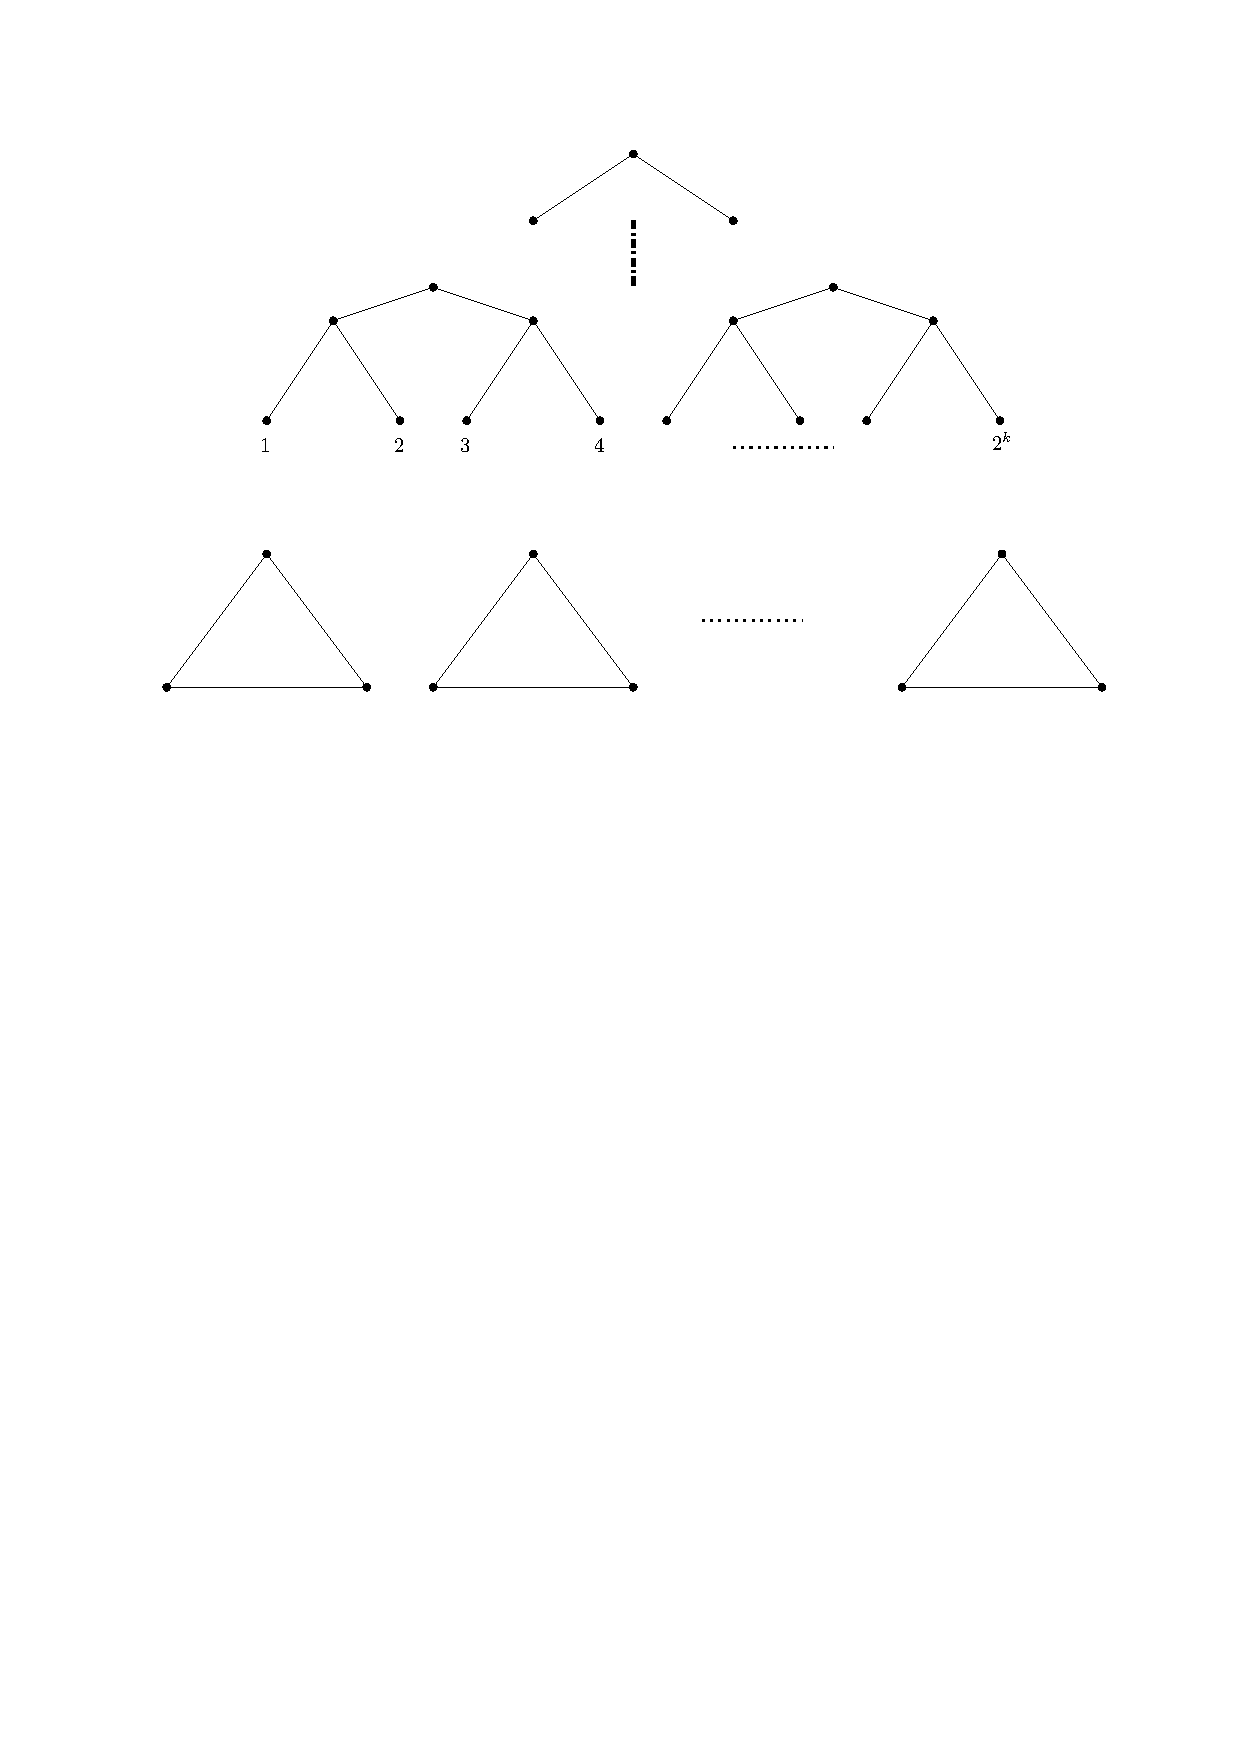
\includegraphics[scale=0.68]{images/transitive}
	\caption{Transitive group action}
	\label{fig:transitive}
\end{figure}

This property of the group action is called Transitive.
\begin{definition}[Transitive Group Action]
	For a group $G \le S_n$ acting on a set $\Omega$, the action is said
	to be transitive if, for all $\alpha, \beta \in \Omega$, there exists
	a $g \in G$ such that $\alpha^g = \beta$.
\end{definition}
In the above example, we can see $Aut(X)$ acts transitively on the set of
leaves of $T$.

Observe that any nontrivial automorphism can either map $1$ and $2$ among
each other (i,e. $1$ to $2$ and $2$ to $1$) or map both $1$ and $2$ to say
$3$ and $4$. But it can never map say $1$ to $2$ and $2$ to $3$ as it violate
adjacency. Hence the leaves with common ancestors always gets moved in a pair.

Consider another graph $X$ which is $k$ vertex disjoint triangles. Consider
the action of $Aut(X)$ on $V(X)$. We again observe a similar phenomena as
before. There is an automorphism that takes any vertex to any vertex. Also
any automorphism maps vertices in a triangle to itself or to a totally 
different triangle. Hence either a triangle is mapped to itself or is moved
whole together as a block.

These two examples motivate the notion of blocks.

\begin{definition}[Blocks]
	For a group $G$ acting on $\Omega$, a set $\Delta \subseteq \Omega$ 
	is a block if $\forall g \in G, \Delta^g = \Delta$ or 
	$\Delta^g \cap \Delta = \phi$.
\end{definition}
We observe that $\Omega$ and the singletons sets $\{\alpha\}$
where $\alpha \in \Delta$ form blocks trivially. 

Apart from the fact that such block structure naturally arise in the action
in many graphs, they also can be potentially used to compute $Aut(X)$. In the
case of trees, we can start with trivial blocks whose automorphisms are also
trivial, combine the blocks and obtain the automorphism for larger blocks and
proceed in a bottom up manner building larger blocks and thereby get the
automorphism of the entire tree.
%\footnote{This is not a rigorous argument and
%is more of an idea to use blocks for computing automorphism.}.

\section{Primitive actions}
We saw that for $\Omega = [n]$ and $G = S_n$, the sets $\Omega$, $\{1\}, \{2\},
\ldots, \{n\}$ does form blocks. Are there any other blocks ? The answer is
no since for any $T \subsetneq \Omega$ of size at least $2$, there is a
permutation in $G$ that fixes one and moves the other. Hence these are the only
blocks and we call such blocks trivial blocks and the action as
\emph{primitive}.

\begin{definition}[Primitive action]
	A group action of $G$ on $\Omega$ is primitive if there are no
	non-trivial blocks. An action which is not primitive is called
	imprimitive.
\end{definition}

Let us consider another action where $G \subseteq S_n$ acts on itself via
right multiplication (see Lecture 8). That is for $g' \in G$, the action
takes $g$ to $gg'$ with $\Omega = G$. This action is clearly transitive as
given any $g,h \in G$, $g' = g^{-1}h$ takes $g$ to $h$. Also, if $G$ has a 
non-trivial \footnote{That is $H$ is not $G$ or $\{id\}$} subgroup $H$ then
the action is not primitive.  This is because, the cosets of $H$ in $G$ form 
the non-trivial blocks. That is, for any two shift of $H$ say $Hg_1, Hg_2$,
either $Hg_1 = Hg_2$ or $Hg_1 \cap Hg_2 = \emptyset$ (Lemma~\ref{lag1}) which
we observed in the proof of Lagrange's theorem.

This shows that if $G$ has a non-trivial subgroup, then the action is not
primitive. Is the converse observation that $G$ has only trivial
subgroup imply the action is primitive also true ? We will see in the next 
lecture that the converse holds too. This gives a very interesting
characterisation or a ``connection'' between blocks which are combinatorial in
nature and subgroups which are algebraic in nature.

We first show that action of $G$ on $\Omega$ induces a partition to form a
block system.

\begin{definition}[Block System]
A partition of $\Omega$ into sets such that each part is a block under the action of G.
\end{definition}

To see this, we will explore some properties of blocks.
\begin{claim}
	Let $G \le S_n$ be a group acting on $\Omega$ and $\Delta \subseteq \Omega$
	be a block. 
	Then for any $g \in G$, the
	following holds.
	\begin{enumerate}
		\item  $\Delta^g$ is also a block
		\item  $|\Delta^g|  = |\Delta|$
	\end{enumerate} \label{cl:block-prop}
\end{claim}
\begin{proof}
	\begin{description}
		\item[Proof of 1] We give a proof by contradiction. Suppose
			there exists a $g \in G$ for which $\Delta^g$ is not a
			block. By definition, since $\Delta^g$ is not a
			block, there exists an $h \in G$ such that 
			\[ \Delta^{gh} \ne \Delta^g \text{ and } 
			\Delta^{gh} \cap \Delta^g \ne \emptyset\]
			Hence there exists $\beta \in \Delta^g$ but $\beta^h
			\not \in \Delta^g$ and there is a $\gamma \in
			\Delta^{gh} \cap \Delta^g$.
			Since $\beta \in \Delta^g$, there exists an $\alpha
			\in \Delta$ such that $\alpha^{gh} \not \in
			\Delta^g$. Hence $\alpha^{ghg^{-1}} \not \in \Delta$
			while $\alpha^{ghg^{-1}} \in \Delta^{ghg^{-1}}$. Hence
			$\Delta \ne \Delta^{ghg^{-1}}$. 

			Since $\gamma \in \Delta^g$ and $\gamma \in
			\Delta^{gh}$, there exists an $\omega,\delta \in 
			\Delta$ such that $\gamma = \omega^g = \delta^{gh}$. 
			Hence $\omega =	\gamma^{ghg^{-1}} \in 
			\Delta^{ghg^{-1}}$. Along with the fact that
			$\omega \in \Delta$, we get that $\Delta \cap
			\Delta^{ghg^{-1}}\ne \emptyset$. But $\Delta \ne
			\Delta^{ghg^{-1}}$ and $\Delta \cap
			\Delta^{ghg^{-1}}\ne \emptyset$ contradicts the fact
			that $\Delta$ is a block. Hence it must be that
			$\Delta^g$ is also a block.
		\item[Proof of 2] 
		This follows from the fact that $g \in G$ is a permutation
		and it is a bijection map.
	\end{description}
\end{proof}

If the group action is transitive, then $\Omega$ is partitioned by the
blocks.
\begin{claim} For a group $G \le S_n$ that acts transitively on $\Omega$ with
	$\Delta \subseteq \Omega$ as a block, the following holds.
	\begin{enumerate}
		\item $\bigcup_{g \in G} \Delta^g = \Omega$
		\item For any $g_1, g_2 \in G$,  $\Delta^{g_1} \cap
			\Delta^{g_2} \ne \phi \Rightarrow \Delta^{g_1} =
			\Delta^{g_2}$.  
		\item $|\Delta|$ must divide $|\Omega|$.
	\end{enumerate}
\end{claim}
\begin{proof}
	\begin{description}
		\item[Proof of 1] 
Let $k \in \Delta$. For any $k' \in \Omega$, since the action is transitive
$\exists g$ such that  $k^g = k'$ giving $k' \in \Delta^g$. Hence $\Omega
\subseteq \bigcup_{g \in G} \Delta^g $. The other containment is direct and
hence they are equal.
		\item[Proof of 2]
		This is true since, with $\Delta^{g_1}$ being a block
		(Claim~\ref{cl:block-prop}(1)), either $\Delta^{g_1} =
		\Delta^{g_1(g_1^{-1}g_2)}$ or  $\Delta^{g_1} \cap
		\Delta^{g_1(g_1^{-1}g_2)} = \emptyset$.
	\item[Proof of 3] The above two claims prove that $\Omega$ is partitioned
		into subsets with equal cardinality and all of them have the
		same size as $|\Delta|$ (Claim~\ref{cl:block-prop}(2)). So
		$|\Delta|$ must divide $|\Omega|$.  \end{description}
\end{proof}

We get an immediate sufficient condition on $\Omega$ for the action of any 
$G$ to be primitive. 
\begin{corollary}
	If $|\Omega |$ is prime, then the action of any $G \le S_n$ on
	$\Omega$ is bound to be primitive.  
\end{corollary}

Before ending, let us see why transitive actions are important. For a general
group $G$ whose action is not necessarily transitive, if we look at the
action on elements of an orbit, the action becomes transitive. Hence we can
use our divide and conquer strategy to build blocks and at least obtain
automorphism group for the orbits.
%\dsay{I am not very clear about this para}

\Lecture{Jayalal Sarma}{Sep 1 2015}{17}{Characterisation of
Primitivity}{Mitali Bafna}{$\gamma$}{K Dinesh}

In the last lecture, we saw transitive and primitive group action. In this
lecture, we give an algebraic characterisation of primitive group actions.

We need the notion of maximal subgroup of a group.
\begin{definition}[Maximal Subgroup]
$H \leq G$ is a maximal subgroup if there does not exist an $H'$ such that 
$H \lneq H' \lneq G$ where $\lneq$ denotes strict subgroup containment.
\end{definition}

The main theorem is the following.
\begin{theorem}
	Suppose $G \le S_n$ acts transitively on $\Omega$. Then the action is
	primitive if and only if $\exists \alpha \in \Omega$ such that
	$G_{\alpha}$ is the maximal subgroup of $G$ where $G_\alpha$ is the
	stabilizer of $\alpha$
	\label{thm:primitive-action}
\end{theorem}

Recall the action (in the last lecture) for $G \le S_n$ where $G$ acts on
itself. We saw that if $G$ has any non-trivial subgroup $H'$, the the action is
not primitive. If $H'$ has a super group $H$ then, there is a nice relation
between the cosets induced by $H$ and $H'$ on $G$ described as an exercise
below.
\printexercise{subgroup-cost-structure}

\begin{figure}[htp!]
	\centering
	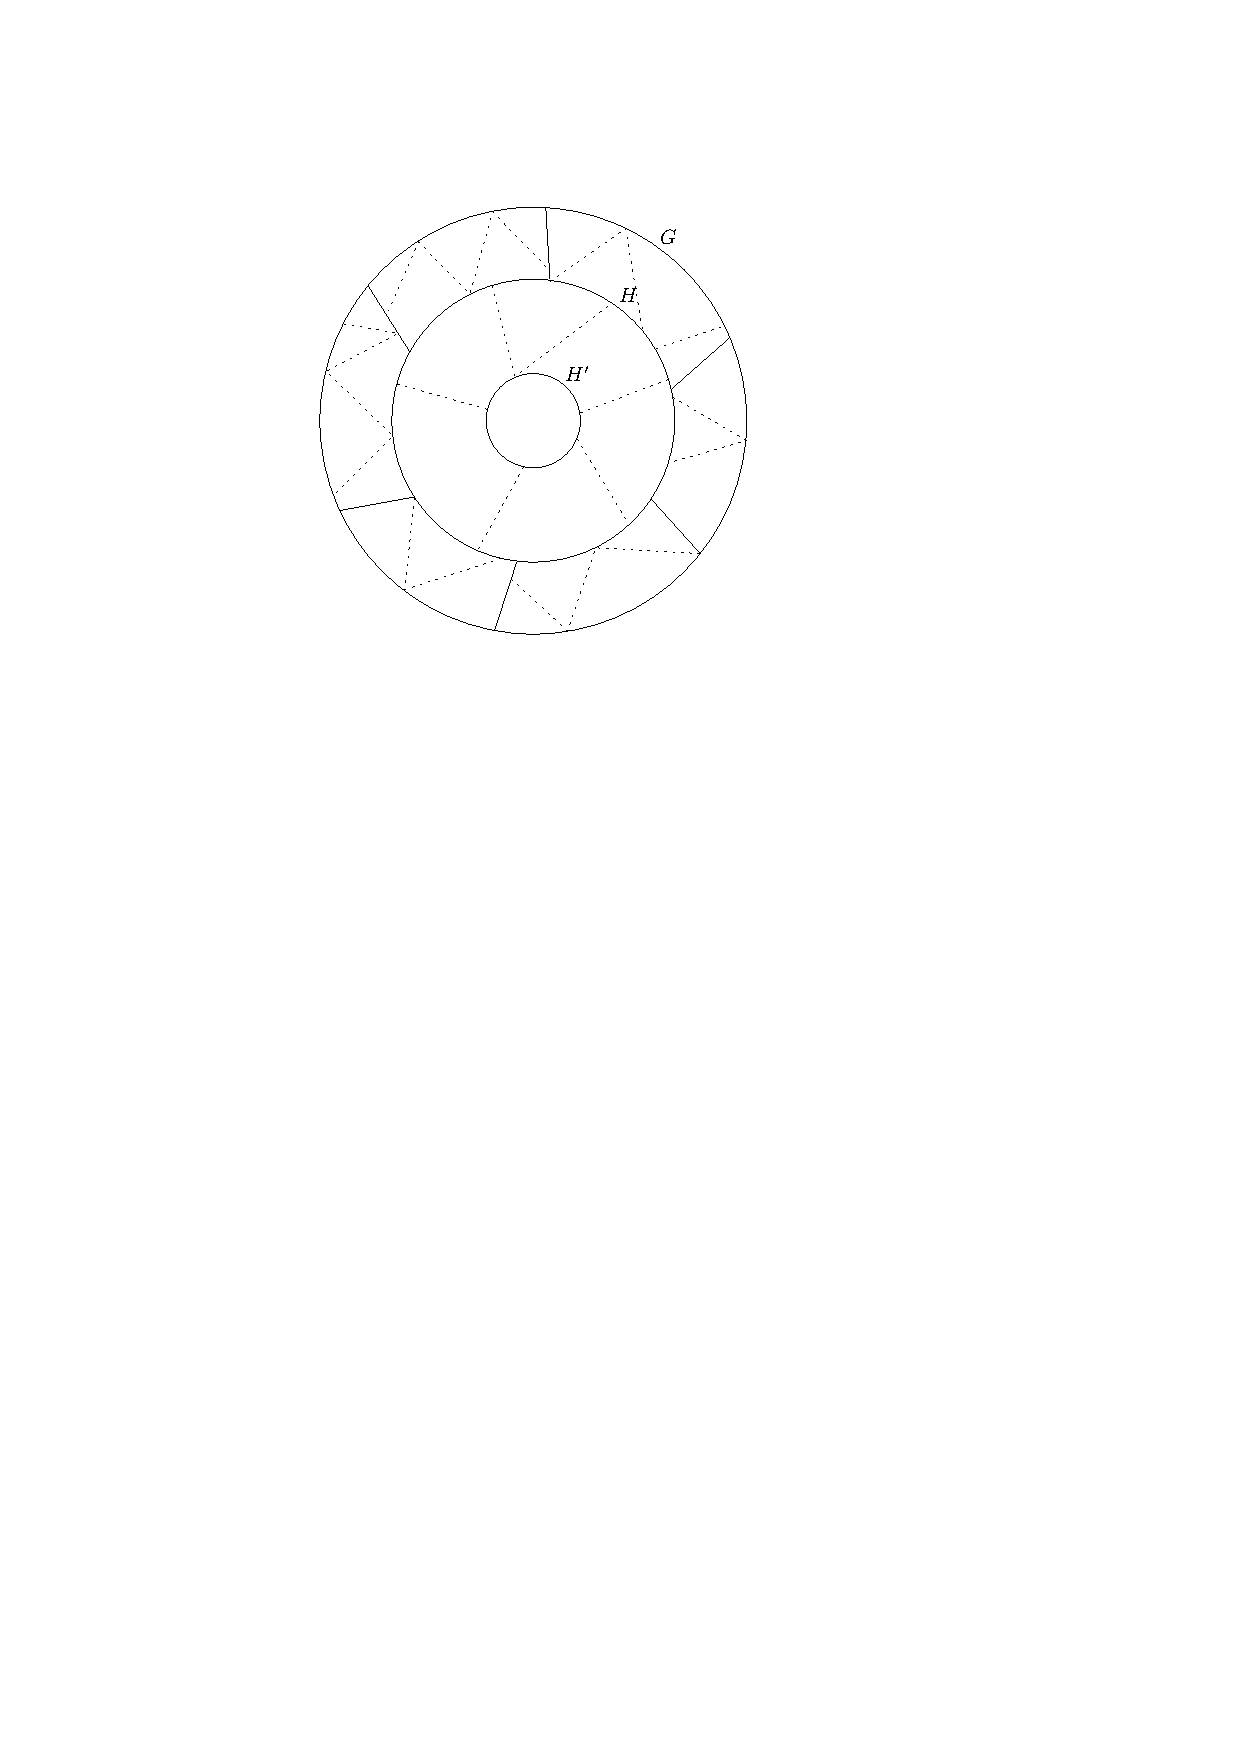
\includegraphics[scale=0.7]{images/coset}
	\caption{Coset structure of subgroups $H$ and $H'$. Dotted ones are
	cosets of $H'$.}
	\label{fig:coset}
\end{figure}

With this structure in place, we can also consider the cosets of $H'$ 
as the elements and consider the action of $G$ on this set. Since $H$ has a
smaller subgroup $H'$, there are non-trivial blocks for this action. The
action moves all those cosets of $H'$ that fall in a coset of $H$. This must
happen as this is precisely the action of $G$ on the cosets of $H$.
Hence the collection of cosets of $H'$ within a cost of $H$ forms a block.
The characterisation theorem for primitive action tells that if $H'$ does not
have a larger subgroup $H$, then the action is bound to be primitive. We state
this as a corollary.

\begin{corollary}
	For $H' \lneq G$ and $H'$ does not have a supergroup $H$ in $G$, the
	action of $G$ on the cosets of $H'$ in $G$ must be primitive.
\end{corollary}

Before going to the proof, we first show that the following variant of 
Theorem~\ref{thm:primitive-action} where $\exists \alpha$ is replaced by 
$\forall \alpha$ is also true. For this, it suffices to prove the following
claim.

\begin{claim}
	For a group $G$ acting transitively on $\Omega$, if there exists an
	$\alpha \in \Omega$ such that $G_\alpha$ is maximal subgroup of $G$,
	then for all $\beta \in \Omega$, $G_\beta$ is also maximal subgroup of
	$G$.
	\label{cl:prop-trans}
\end{claim}
\begin{proof}
	Suppose there exists $\alpha$ such that $G_\alpha$ is maximal subgroup
	of $G$. Since $G$ is transitive, for any $\beta \in \Omega$, there
	exist a $g$ such that $\alpha^g = \beta$. Note that $G_\alpha$ and
	$G_\beta$ can be related as $g^{-1}G_\alpha g =
	G_\beta$. This is because,
	\begin{align*}
		G_\beta  =&  \{ g' ~|~ \beta^{g'} = \beta \} \\
			= & \{ g' ~|~ \alpha^{gg'} = \alpha^g \} \\
			= & \{ g' ~|~ \alpha^{gg'g^{-1}} = \alpha \} \\
			= & \{ g^{-1} hg ~|~ \alpha^{h} = \alpha \} &&
			[\text{Renaming $gg'g^{-1}$ as $h$}] \\
			= & g^{-1}G_\alpha g
	\end{align*}
	Now if $G_\beta$ has a larger subgroup containing
	it in $G$, then we can give a larger
	subgroup for $G_\alpha$ also which contradicts maximality\footnote{ If
		there is an $H'$ such that $G_\beta \lneq H' \lneq G$ then
		consider $g^{-1}H'g$ as it satisfy $G_\alpha \lneq g^{-1}H'g
	\lneq G$.}. 
\end{proof}
The pair of groups $G_\alpha$, $G_\beta$ in the previous claim are sometimes
called as conjugate pairs.
\begin{definition}[Conjugates]
	Subgroups $H,H'$ of a group $G$ are said to be conjugates, if there 
	exists a $g \in G$ such that $gHg^{-1} =H'$.
\end{definition}

\section{Proof of characterisation}
We restate the characterisation in the light of Claim~\ref{cl:prop-trans}.
\begin{theorem}
	Suppose $G \le S_n$ acts transitively on $\Omega$. Then the action is
	primitive if and only if $\forall \alpha \in \Omega$ such that
	$G_{\alpha}$ is the maximal subgroup of $G$ where $G_\alpha$ is the
	stabilizer of $\alpha$
	\label{thm:primitive-action-strong}
\end{theorem}
Note that both these theorems are equivalent. We now give a proof.

\begin{proof}[Proof of Theorem~\ref{thm:primitive-action-strong}]

The backward direction ($\Longleftarrow$): if $\forall \alpha \in G$,
$G_\alpha$ is maximal the maximal subgroup of $G$, then the action is
primitive.

We will prove the contrapositive that is, suppose that the action is not 
primitive then $\exists \alpha \in G$ such that , $G_\alpha$ is not a maximal 
subgroup.

Suppose $G$ does not act primitively on $\Omega$. Then there must be
non-trivial block $\Delta$ and $\alpha \in \Omega$ such that $\{\alpha\}
\subsetneq \Delta \subsetneq \Omega$. We need to show that there exists an $H$
such that $G_\alpha \lneq H \lneq G$. We show this in two steps.

\begin{description}
	\item [Show that $G_\alpha \le H \le G$ :]
Consider $H = \setstab(\Delta) = \{g \in
G ~|~ \Delta^g =\Delta \}$. We now show that $G_\alpha$ is a subgroup of $H$.
To show this, let $g \in G_\alpha$. Hence $\alpha^g = \alpha$ and $\alpha$ is
a common element in $\Delta$ and $\Delta^g$. Along with the fact that $\Delta$
is a block, we get that $\Delta = \Delta^g$. Hence $g$ fixes $\Delta$ which
gives that $g \in H$.  Hence $G_\alpha \leq H$. By definition of $H$, we have $H \le G$.
	\item [Both containments are strict :]
Let $\beta \neq \alpha$ belongs to $\Delta$. Such a $\beta$ must exist as
$\{\alpha\} \subsetneq \Delta$. Since $G$ is transitive, there exists a  $g
\in G$ such that $\alpha^g = \beta$.  Clearly 
$g \notin G_\alpha$. Now since $\beta \in \Delta \cap \Delta^g$ and $\Delta$
is a block, we get $\Delta^g = \Delta$ and $g \in H$.
\end{description}
Hence $G_\alpha \lneq H \lneq G$ and $G_\alpha$ is not maximal.

The forward direction ($\Longrightarrow$):
We again prove the contrapositive : if $\exists \alpha \in \Omega$ such that 
$G_\alpha$ is not a maximal subgroup, then the action is not primitive (i,e.
come up with a non-trivial block).

Suppose $\alpha \in \Omega$ be such that $G_\alpha \lneq H \lneq G$.  We will
produce a $\Delta$ such that $\Delta$ is a non-trivial block. We define 
$\Delta = \alpha^H$. Now we are left to show that the $\Delta$ chosen is
indeed a non-trivial block. To prove this, we need to show the following:
\begin{description}
	\item[$\{\alpha\} \subsetneq \Delta$ :] 
		From the Orbit-Stabiliser lemma (Lemma~\ref{lem:os}), we have
		that each coset of $G_\alpha$ in $G$ corresponds to a
		different element in the orbit of $\alpha$.  That is all the
		elements in a coset take $\alpha$ to the same element and if
		two cosets are different then their action on $\alpha$ is too.
		Mathematically, for $g_1,g_2 \in G$, 
		$g_1G_\alpha = g_2G_\alpha \Leftrightarrow
		\alpha^{g_1} = \alpha^{g_2}$.

	Since $G_\alpha \lneq H,\exists$ a coset $C \neq G_\alpha \in H$. Let
	$C = G_\alpha h$ where $h \in H$ is the coset representative.
	Now, $G_\alpha \neq C \Rightarrow \alpha  \ne
	\alpha^h = \beta$ for some $\beta \in \Omega$. But $\beta = \alpha^h
	\in \alpha^H = \Delta$.  So we have that $\{\alpha\} \subsetneq
	\Delta$.
	% proof done in class:
	%	Since $G_\alpha \lneq H$,
	%	there exists $g \in H$ such that $ g\not \in G_\alpha$. Hence
	%	$\alpha^g = \beta$ where $\beta \ne \alpha$. Also $\beta \in
	%	\Delta$ as $\beta$ is in the orbit of $g$. Hence $\{\alpha
	%	\} \subsetneq \{\alpha, \beta\} \subseteq \Delta$.

	\item[$\Delta \subsetneq \Omega$ :] 
	Since $H \lneq G$ and $G_\alpha \lneq H, \exists$ a coset $C$ of
	$G_\alpha$ in $G$ which does not belong to $H$. Let $g \in G$ be its
	coset representative. Since different cosets
	take $\alpha$ to different elements $\alpha^g \notin \alpha^H$. So we
	have that $\Delta = \alpha^H \subsetneq \alpha^G = \Omega$. 

	\item[$\Delta$ is a block :]
		We show that for any $g \in G$, either $\Delta^g = \Delta$ or
		$\Delta^g \cap \Delta = \emptyset$. Suppose $\Delta^g \cap
		\Delta = \emptyset$, we are done. Suppose $\Delta^g \cap
		\Delta \neq \emptyset$. We then show that $\Delta^g = \Delta$.
		
		Recall that $\Delta = \alpha^H$. Since $\Delta^g \cap \Delta
		\ne \emptyset$, 
		\begin{align*}
		& \exists h',h \in H, \alpha^{h'g} = \alpha^h \\ 
		\implies & h'gh^{-1} \in G_\alpha \\
		\implies & g \in H && [\text{Using $G_\alpha$ is a subgroup of
		$H$}] \\
		\implies & \Delta^g = \alpha^{Hg} = \alpha^H = \Delta
		\end{align*}
\end{description}
This completes the proof.
\end{proof}






\Lecture{Jayalal Sarma}{*Month, XX 2015*}{18}{*Title of Lecture*}{*Student
name*}{$\alpha$}{TA}

\begin{note}
	Enter date, lecture number, title and your name. 
\end{note}
\jsay{This is a sample comment}

\section{Sample section}
This is a sample section. Sections helps in dividing the notes to logically separated parts.


\section{Writing Math}
Here we will see how to write math. Normal math symbols : 
$\alpha\beta\gamma\epsilon\phi\Phi $. You can also use calligraphic letters : $\calC$
\begin{enumerate}
\item Avoid these : B=A2+B*ci, B $=$ A $+$ B $*$ c$_i$, phi:A -> N
\item Good math : $B=A^2 +~~~B \times c_{ij}$, $\phi: A \leftarrow N$. Note the space in the equation.
\end{enumerate}



\section{Writing Theorems and Proofs} \label{sec:rel}
\begin{theorem} \label{cl:relativity}
If $m$ is mass and $c$ is speed of light then, 
\begin{equation} \label{eq:relativity}
E = mc^2
\end{equation}

\end{theorem}
\begin{proof}
Trivial. 
\end{proof}

\begin{claim} 
Halting problem is undecidable
\end{claim}
\begin{proof}(Idea)
Set of languages is $\mathcal{P}(\Sigma^*)$ is uncountably infinite,
while set of all Turing machines which can be identified with 
$\Sigma^*$ is only countably infinite. 

If Halting problem is 
decidable, then every language in $\mathcal{P}(\Sigma^*)$ can be 
captured uniquely by Turing machines. This suggests existence of a 
bijection. But such a bijection between a countably infinite 
and uncountably infinite set cannot exits by Cantor's diagonalisation argument. 
Hence Halting problem is undecidable.
\end{proof}

\subsection{Environments available}
\begin{proposition}
This is a proposition.
\end{proposition}
\begin{corollary}
	This is a corollary
\end{corollary}
\begin{observation}
	This is an observation
\end{observation}
\begin{definition}
	This is a definition
\end{definition}
\begin{example}
	This is an example
\end{example}
\begin{exercise}
	This is an exercise
\end{exercise}
\begin{remark}
	This is a remark
\end{remark}
\begin{conjecture}
	A conjecture
\end{conjecture}

\begin{fact}
	A fact
\end{fact}


\subsection{Writing equations}
\begin{itemize}
\item Normal equations : 
	$\int_0^\infty e^{-x} x^{n-1} \mathrm{d}x = \Gamma(n)$.
\item Display math equation : 
	\begin{equation}
	\int_0^\infty e^{-x} x^{n-1} \mathrm{d}x = \Gamma(n)
	\end{equation}
\item Display math equation with no numbering : 
	\begin{equation*}
	\int_0^\infty e^{-x} x^{n-1} \mathrm{d}x = \Gamma(n)
	\end{equation*}
\item Writing sets and using $\langle$ $\rangle$ instead of $<$ and $>$
	\begin{equation}
	HP = \set{ \langle M,x \rangle ~|~ \text{$M$ on inputs $x$ halts} }
	\end{equation}
	\begin{equation}
	S =  \set{ i ~\left |  \prod_{d | i} i \text{ is even }, i > 0 \right . }
	\end{equation}
\end{itemize}

\subsection{Aligning equations, writing text in math mode}
\begin{align*}
\sum_{i=1}^n i & = \sum_{i=1}^{n-1} i + n \\
			   & = \frac{(n-1)\cdot n}{2} + n && [\text{By induction hypothesis}]\\
			   & = \frac{n(n+1)}{2}
\end{align*}




\section{Drawing tables}
\begin{center}
\begin{tabular}{||c|l|l||}
\hline 
\textbf{Type} & \textbf{Language} & \textbf{Machine} \\ 
\hline \hline
Type 3 & Regular & Finite Automata \\ 
\hline 
Type 2 & Context Free & Push Down Automata \\ 
\hline 
Type 1 & Context Sensitive & Linear Bounded Automata \\ 
\hline
Type 0 & Recursively Enumerable & Turing Machine \\ 
\hline 
\end{tabular} 
\end{center}

\section{Referring sections and theorems}
Recalling equation~\ref{eq:relativity} in claim~\ref{cl:relativity} from section~\ref{sec:rel},
it is possible to generate energy from nuclear reactions.




\Lecture{Jayalal Sarma}{*Month, XX 2015*}{19}{*Title of Lecture*}{*Student name*}{$\alpha$}{TA}

\section{Add details of next lecture}

\Lecture{Jayalal Sarma}{Sep 5, 2015}{20}{Reduction from Trivalent Graph Isomorphism to Restricted Set Stabilizer Problem}{Jayalal Sarma}{$\alpha$}{Jayalal Sarma}


\Lecture{Jayalal Sarma}{September, 08 2015}{21}{Structure of groups for
d-degree graphs}{Sanjay Ganapathy}{$\alpha$}{K Dinesh}

In the previous lecture, we were interested in finding the generating set for
the automorphism group of X which is given to be a graph bounded by maximum
degree 3. We in turn reduced this problem to solving the set stabilizer
problem for the special case where the group is a 2-group that is $|G|$ =
$2^{k}$.  Given G, a 2-group acting on $\Omega$ and $\Delta \subseteq \Omega$,
find the generating set of setstab ($\Delta$). In order to solve the set
stabilizer problem for this group, first we shall charaterise the structure of
groups for graphs with maximum degree d.

\begin{definition}[\textbf{Composition Series}]

If a given group G has a sequence of subgroups $G_{1}$, $G_{2}$, ... $G_{k}$, such that \\
G = $G_{0} \triangleright G_{1} \triangleright G_{2}$ ... $\triangleright G_{k}$ = \{identity\} \\
and $\forall$ i, $G_{i+1}$ is a maximal strict normal subgroup of $G_{i}$, then such a series is referred to as a composition series of G.

$G_{i+1} / G_{i}$ is called composition factor.
\end{definition}

\begin{claim}
If a graph X has maximum degree $\leq$ d, then $Aut_{e}(X)$ has a composition series with quotient groups isomorphic to $S_{d-1}$.
\end{claim}

However our interest is in the case when d = 3 and $Aut_{e}(X)$ is a 2-group. We will make use of Sylow's theorem to prove the existence of a composition series for such a group where the size of each subgroup $G_{i}$ will be $2^{k - i}$ where $k$ is such that $|G| = 2^{k}$. 

\section{Sylow's Theorem}

\begin{theorem}[\textbf{Sylow's Theorem}]
If G is a group of size $p^{m}r$ where p is a prime and r is such that gcd (p,r) = 1, then $\exists$ H, such that $H \leqslant G$ and $|H|$ = $p^{m}$
\end{theorem}

However, this version of Sylow's theorem is not directly applicable to our problem, since in our problem, $|G| = 2^{k}$. Instead, we prove this restated version of Sylow's theorem.

\begin{theorem}
If $p^{l} \; | \; |G|$ then there exists a subgroup of size exactly $p^{l}$ for G.
\end{theorem}

\begin{proof}

Consider $|G|$ = $p^{m}r$ where $p^{k}$ divides r but $p^{k+1}$ does not divide r.

Consider the set $\Omega$ = \{ set of all subsets of G of size $p^{m}$ \}. Note this is not the $\Omega$ referred to at the starting of the lecture.

Action of g $\in$ G on any subset of size $p^{m}$ (assume action by left multiplication) will take the subset to some other subset of size $p^{m}$, that is it will be another element belonging to $\Omega$.

Consider A $\in$ $\Omega$, that is A is such that A $ $ G and $|A|$ = $p^{m}$.

$$ A^{g} = \{\; ga\; | \; a\; \in \; A \;\} $$
We know that
$$ |\Omega| = {p^{m}r \choose p^{m}} $$

\begin{theorem}[\textbf{Lucas's Theorem}]
If there is a prime p and positive integer r, such that gcd (p,r) = 1, then p $\nmid$ ${p^{m}r \choose p^{m}}$
\end{theorem}

This can be extended for the case where gcd (p,r) $\neq$ 1, as follows.
\begin{theorem}
If there is a prime p and postive integer r such that $p^{k} \;|$ r and $p^{k+1}$ $\nmid$ r, then $p^{k+1}$ $\nmid$ $p^{m}r \choose p^{m}$. 
\end{theorem}
\begin{proof}
The proof is quite simple. We just have to expand the term $p^{m}r \choose p^{m}$
\[  {p^{m}r \choose p^{m}} = \frac{p^{m}r \times (p^{m}r - 1) \times (p^{m}r - 2) ... \times (p^{m}r - (p^{m} - 1))}{p^{m} \times (p^{m} - 1) \times (p^{m} - 2) ... \times (p^{m} - (p - 1))} \]
We directly observe a natural numerator-denominator pair structure emerge. We know $p^{k}$ divides r. So, we just have to prove p does not divide the remaining number. Consider any numerator-denominator pair:
$$ \frac{p^{m}r - i}{p^{m} - i} $$
If $p^{\alpha}$ divides the numerator, we know $\alpha$ is definitely less than m because $i < p^{m}$, and $p^{m}$ cannot divide the numerator. So, if $p^{\alpha}$ divides the numerator, we observe that it will also divide the denominator. This follows from the observation that $p^{m}$ is divisible by $p^{\alpha}$ and so i must also be divisible by $p^{\alpha}$. Therefore $p^{m} - i$ is also divisible by $p^{\alpha}$. Thus p does not divide the remaining number and so $p^{k+1}$ does not divide $p^{m}r \choose p^{m}$. 
\end{proof}

Consider $\theta_{1}$, $\theta_{2}$, ..., $\theta_{K}$ to be the orbits of $\Omega$.
\[ \implies |\Omega| = |\theta_{1}| + |\theta_{2}| + ... + |\theta_{K}| \]
Since $p^{k+1}$ does not divide LHS, there exists at least one $i$ such that $p^{k+1}$ does not divide $|\theta_{i}|$. Since $A \in \theta_{i}$, orbit(A) = $\theta_{i}$.

Consider the pointwise stabilizer of A, $G_{A}$. We know from orbit-stabilizer lemma that
\[ |orbit(A)| \times |G_{A}| = |G| \]

$p^{m+k}$ divides the RHS. We know $p^{k+1}$ does not divide orbit(A). Therefore $|G_{A}|$ must be divisible by $p^{m}$. We'll now proceed to show that $|G_{A}|$ is in fact equal to $p^{m}$.

\begin{claim}
\[ |A| \geq |G_{A}| \]
\end{claim}

\begin{proof}
Suppose $|G_{A}|$ $>$ $|A|$. We know any element $g \in G_{A}$ stabilizes A, that is every element A is mapped to some other element in A, by action of $g$ by left multiplication. Let's take an element $g_{i}$ belonging to $A$. There are at most $|A|$ different elements that $g_{i}$ can go to. Since $|G_{A}|$ > $|A|$, by pigeon hole principle we have that there exists at least 2 elements, say $g_{j}$ and $g_{k}$ belonging to $G_{A}$ such that they map $g_{i}$ to the same element say g'.
\[ g_{j} * g_{i} = g_{k} * g_{i} \]
By right multiplication with $g_{i}^{-1}$ on both sides, we will get that $g_{j}$ and $g_{k}$ are in fact equal. Thus, we arrive at a contradiction.
\end{proof}

Since $|A|$ = $p^{m}$, this implies
\[ p^{m} \; | \; |G_{A}| \text{ and } p^m \geq |G_{A}| \]
Therefore $|G_{A}| = p^{m}$. Thus for any $p^{l}$ such that $p^{l}$ divides $|G|$, we can prove the existence of a subgroup of size $p^{l}$.

Coming back to our original problem of proving the existence of a compostion series for $Aut_{e}(X)$, since this is a 2-group of size $2^{k}$, by Sylow's theorem we know that a normal subgroup of size $2^{k-1}$ exists for $Aut_{e}(X)$. We can inductively extend this proof to each subgroup, $G_{i}$ and thus prove the existence of a compostion series.

In general, for any group G, G $\in$ $B_{d}$ if there exists a chain of normal subgroups such that each compostion factor is isomorphic to $S_{d-1}$. We call such a group to be structured. For the trivalent graph case, d = 3 and hence the compostion factor is isomorphic to $S_{2}$, which is what we have shown. Here $S_{d-1}$ refers to a symmetric group on $d - 1$ elements.
\end{proof}

\section{Structure Forests}

We will solve the problem of finding a generating set for setstab ($\Delta$) using a recursive algorithm on a structure tree.

\subsection{Motivating Structure Trees}

Consider the same complete binary tree of depth $k$ we had used while motivating groups and transitive actions, where we consider the existence of a group $G$ such that $G \leqslant S_{n}$ and $G$ acts transitively on $\Omega$, where $\Omega$ is the set of leaves. Each internal node of the tree can be thought of as corresponding to a subset of $\Omega$, which is a block. In general, when we have two vertices $u$ and $v$ such that $u$ is the child of $v$, the following condition holds:
\begin{center}
$u$ is a child of $v$ if $\Delta_{u}$ is a maximal block in $\Delta_{v}$. It means that there does not exist a $\Delta$ such that $\Delta_{u}$ $\subset$ $\Delta$ $\subset$ $\Delta_{v}$ 
\end{center}

\begin{observation} 
When $G$ is general, you get a structure forest, with each tree corresponding to an orbit. This follows from the fact that G acts transitively on an orbit by definition. 
\end{observation}

In the next lecture, we'll formally define structure forests and use them to formulate a recursive solution for the restricted set stabilizer problem and prove that the running time of the algorithm is bounded by a polynomial for $d$ degree graphs.

\Lecture{Jayalal Sarma}{September, 09 2015}{22}{Solving Restricted Set
Stabilizer Problem}{Sanjay Ganapathy}{$\alpha$}{K Dinesh}

We will formalise the notion of structure forests that we motivated in the last lecture.

\section{Structure Forests}
\begin{enumerate}
\item Each tree in the forest corresponds to one orbit.
\item Leaves are the elements of $\Omega$, internal nodes correspond to blocks and roots correspond to orbits.
\item A vertex $u$ is a child of vertex $v$ if $\Delta_{u}$ is a maximal block in $\Delta_{v}$.
\end{enumerate}

\begin{figure}[htp!]
	\centering
	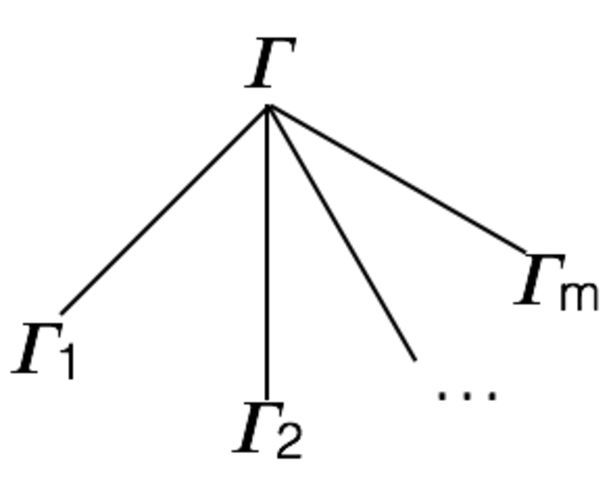
\includegraphics[scale=0.5]{images/structuretree.pdf}
	\caption{Each $\Gamma_{i}$ is a maximal block in $\Gamma$.}
	\label{fig:structurestree}
\end{figure}

\begin{claim}
Action of G on the set ${\Gamma_{1}, \Gamma_{2}, ..., \Gamma_{m}}$ is primitive.
\end{claim}
\begin{proof}
Consider action of G on the set \{1, 2, 3, ... m\}. Suppose there was a non-trivial block $\delta$ such that
\[ \delta \subset \text{ \{1, 2, ... m\}} \]
\[ |\delta| \; \neq \; 1 \]
\[ \delta^{G} \cap \delta = \phi \text{ or } \delta^{G} = \delta \]
\[ B = \bigcup_{i \in \delta} \Gamma_{i} \]
Thus, B is a block such that $\Gamma_{i}$ $\subset$ B $\subset$ $\Gamma$. But this contradicts the existence of the edge $\Gamma$ - $\Gamma_{i}$.
\end{proof}

Consider the partition of $\Omega$ into it's orbits.
$$ \Omega = \Omega_{1} \cup \Omega_{2} ... \cup \Omega_{k} $$

\begin{observation}
It suffices to find the setstab of $\Delta\cap\Omega_{i}$ separately and take the union.
\end{observation}

This is because, there does not exist a group element $g$ which can take any element belonging to $\Omega_{i}$ to $\Omega_{j}$ where $i \neq j$, by virtue of the two elements being in different orbits. Thus when $\Delta$ is stabilized, elements belonging to an orbit are also constrained to remain in the same orbit.

Thus we have reduced our original problem to finding the generating set of $\Delta\cap\Omega_{i}$. Thus hereon, we will focus on one orbit and refer to it as $\Omega$ and $\Delta\cap\Omega$ as $\Delta$.

\section{Algorithm for computing setstab($\Delta$)}

\begin{figure}[htp!]
	\centering
	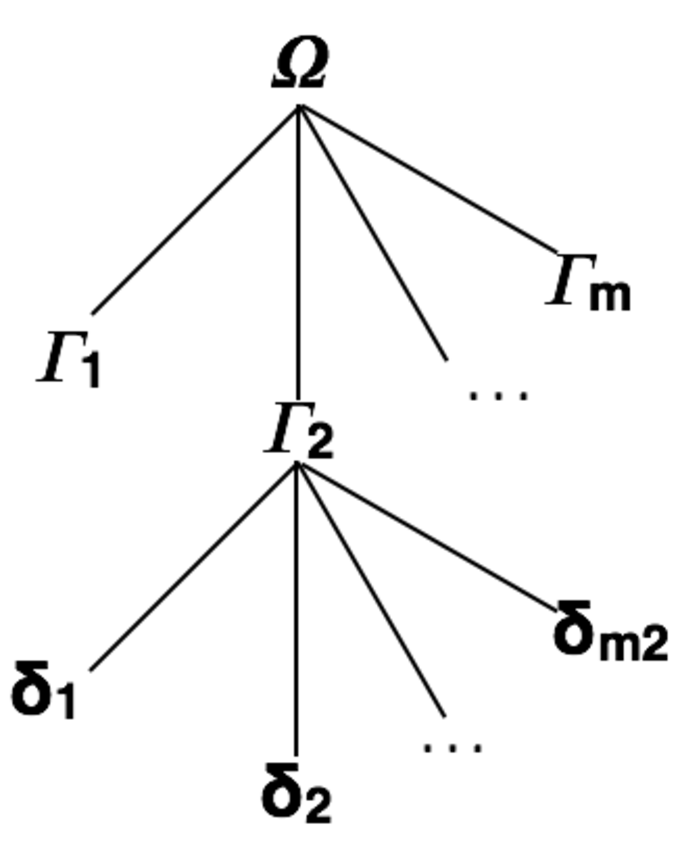
\includegraphics[scale=0.3]{images/setstabalg.pdf}
	\caption{Structure tree for one orbit of $\Omega$ under the action of G.}
	\label{fig:structurestree}
\end{figure}

Consider $H$ = \{ $g$ $\in$ $G$ $|$ $\forall$ $i$ $\Gamma_{i}^{g}$ = $\Gamma_{i}$ \}. $H$ is the setwise stabilizer of $\Gamma_{i}$. This means we can write G in terms of the cosets of $H$. 


\begin{figure}[htp!]
	\centering
	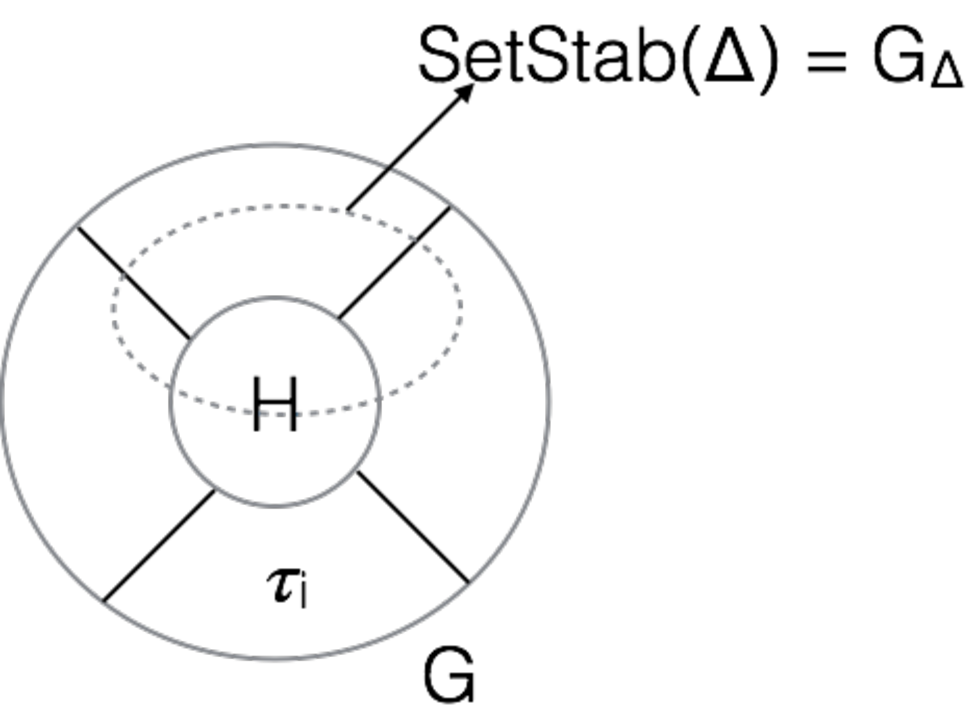
\includegraphics[scale=0.5]{images/setstabgroup.pdf}
	\caption{Set Stabilizer group of $\Delta$ in G and the cosets of $H$, which is the setwise stabilizer of $\Gamma_{i}$.}
	\label{fig:setstabgroup}
\end{figure}

\[ G =  \bigcup_{i=1}^kH\tau_{i} \]
\[ G_{\Delta} = \bigcup_{i=1}^k(H\tau_{i})_{\Delta} \]

We need to find the elements in each coset of $H$, which stabilizes $\Delta$. This leads to a natural recursive formulation which we formalise below. 

\subsection{Generalized Set Stabilizer} 
Given $\Delta$, $H$ and $\sigma$, such that $H$ stabilizes $\Omega'$, where $\Omega'$ $\subseteq$ $\Omega$, find $(H\sigma)_{\Delta}$. 

If we visualize $\Delta$ to be a 2 colouring on the elements of $\Omega$, then we can write
\begin{center}
SetStab (H, $\sigma$, $\Omega'$) = \{$h$ $\in$ $H\sigma$ $|$ $\forall$ $\omega$ $\in$ $\Omega' \text{ $\omega$ and $\omega^{h}$ has the same colour}$\}
where $\Omega'$ is one of $\Gamma_{i}$.
\end{center}

Therefore, we need to recursively solve SetStab($\Gamma_{i} \cap \Delta, \sigma$), for each level of the tree. To show that this algorithm runs in polynomial time, we make use of the following bound.

\begin{theorem}[\textbf{Babai Luke Palfy Bound}]
If $G \leqslant S_{n}$ is a structured group, then $|G|$ is bounded by $n^{c}$  for some constant c.
\end{theorem}

We have already proved that $Aut_{e}(X)$ is a structured group, for a d-degree bounded graph. Thus, we can use this theorem to show that $|G| \leq n^{cd}$. Thus the number of nodes in the tree is polynomial and number of coset representatives is also polynomial since the size of the group itself is bounded by a polynomial. Thus, since the recursion only visits each node of the tree once, and the computation per node is bounded by a polynomial, the entire algorithm is of polynomial order.

More precisely, we can show that we can solve the graph automorphism problem in $O(n^{d^{2}})$ time.

In the next lecture, we will try to refine the trivial brute force algorithm of finding a graph isomorphism between 2 graphs $X_{1}$ and $X_{2}$ and develop an algorithm which runs in $O(n^{n^{\frac{2}{3}}})$.


K Dinesh\Lecture{Jayalal Sarma}{September, 11 2015}{23}{General Graph Isomorphism}{Vidhya Ramaswamy}{$\beta$}{K Dinesh}

\section{Introduction}
In these set of lectures, we consider the general graph isomorphism problem, and improve the solution. We know that we have a trivial solution in $O(n^n)$ time, by checking all possible mappings from graph $X_1$ to graph $X_2$. In the previous lecture, we have shown that when the graphs have a degree $d$ bound, we have an $O(n^{d^2})$ time solution.
\\We now give a $O(n^{n^{\frac{2}{3}}})$ bound for solving the general graph isomorphism problem.

\section{Colourings and Refinements of Colourings}
A colouring of a graph is a function mapping vertices of a graph to integers.
\[
f: V \longrightarrow \{1, 2, ... |V|\}
\]
To make understanding easier, we assume that $Range(f)$ is some initial segment of $\{1, 2, ... |V|\}$. That is, if we assign $k$ colours to all the vertices, we assume that the $k$ colours used are $\{1, 2, ... k\}$.
\paragraph*{}
We now introduce the idea of a Refinement of a Colouring. We can understand the idea of a refinement empirically as follows. Consider a colouring $f$ of a graph $X$. This partitions the graph into some colour classes. Now, we say that $g$ refines $f$ if $g$ further partitions each of these colour classes. 
\\Formally, we define refinement as follows:
\begin{definition}
We say that a colouring $f_1$ refines a colouring $f_2$ if $\forall x, y \in V$,
\[
f_2(x) \le f_2(y) \Rightarrow f_1(x) \le f_1(y)
\]  
\end{definition}
We write this as $f_1 \le f_2$
\section{Algorithm}

We notice that if we colour the graphs such that any isomorphism between the graphs would preserve the colouring, then, our job of finding an isomorphism becomes potentially easier, especially if each of the colour classes have very few vertices in them.
\paragraph*{}
We do this by choosing a colouring which preserves the degree information. 
\begin{enumerate}
\item Initially, all vertices are coloured with the same colour.
\item At each step, we refine this colouring, by encoding the number of vertices of a particular colour which are its neighbours. 
\item We continue this refinement process until no changes are made in the colouring. We call this a \textbf{stable colouring} of the graph.
\end{enumerate}
\paragraph*{}
Formally, we describe the refinement process as follows:\\
Let $f$ be a colouring, mapping a vertex $x$ to colour $f(x)$, using $k$ colour classes. Now, we describe $g$ (the refinement of $f$) as follows.
\begin{eqnarray*}
g(x) = (f(x), \chi_1(x), \chi_2(x), ... & \chi_k(x))
\end{eqnarray*}
where $\chi_i(x)$ = Number of neighbours of $x$ in colour class $i$.\\  
We can now order the tuples in some order (maybe lexicographic) and then map them to $\{1, 2, ... |V|\}$.\\
As we encode $f(x)$ in the beginning of $g$, $g$ is obviously a refinement of $f$.
\paragraph*{}
\begin{definition}
We say that 2 vertices are \textbf{not distinguished} if they are in the same colour class for a stable colouring.
\end{definition}
When we get a stable colouring, we observe the following:
\begin{observation}
For 2 vertices to be not distinguished, they have the same degree within each colour class. 
\end{observation}
\begin{observation}
When the colouring is stable, 
\begin{enumerate}
\item The induced graph of any colour class is regular.
\item The bipartite graph between any 2 colour classes is semi-regular. That is, each vertex in the left partition has the same degree, each vertex in the right partition has the same degree, but these degrees need not be the same.
\end{enumerate} 
\end{observation}

\textbf{Note: }If 2 vertices are not distinguished, this does \textbf{not} imply that an automorphism mapping one vertex to the other is possible. 
Consider figure \ref{fig:StableColouringNotIsomorphic6} below. As every vertex in this graph has a degree 3, the refinement process stops after one pass, and all vertices are coloured with the same colour.
However, there is no automorphism mapping vertex 1 to vertex 3.
\begin{figure}[htp!]
	\centering
	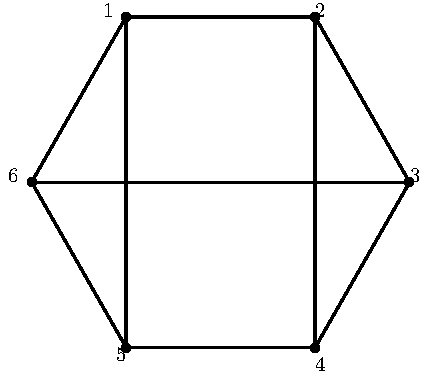
\includegraphics[scale=1]{images/not_iso.pdf}
	\caption{No automorphism mapping vertex 1 to 3}
	\label{fig:StableColouringNotIsomorphic6}
\end{figure}
\\We can also see an example where all vertices are in the same stable colour class, but there are no non-trivial isomorphisms (See \ref{fig:StableColouringNotIsomorphic12}) .
\begin{figure}[htp!]
	\centering
	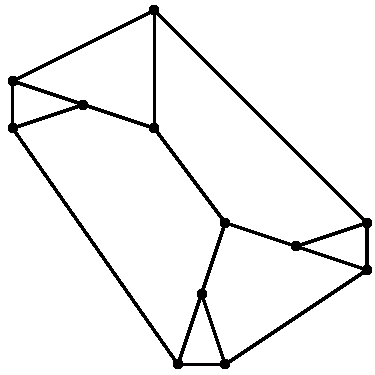
\includegraphics[scale=1]{images/not_iso12.pdf}
	\caption{No non-trivial automorphism}
	\label{fig:StableColouringNotIsomorphic12}
\end{figure}



\paragraph*{}
We claim that this process of refinement does not lose any isomorphisms. That is, 
\begin{claim}
If $f_1 \le f_2$, 
\[
(X_1, f_1) \cong (X_2, f_1) \Leftrightarrow (X_1, f_2) \cong (X_2, f_2)  
\]
\end{claim}
We leave the proof of this claim as an exercise to the reader.

\paragraph*{}
If, after obtaining a stable colouring, we have only one vertex in each colour class, we are done, as this forces each vertex to be mapped to a specific vertex in the other graph. 
If not, we force singleton colour classes by the idea of \textbf{Individualisation}.

\subsection{Individualisation}
For individualisation, we do the following.
\begin{enumerate}
\item Choose any vertex $x$ such that it is not in a singleton colour class, and colour it with a new colour.
\item Refine the colouring, until we get a stable colouring again. 
\item Repeat steps 1 and 2 until we get singleton colour classes.
\end{enumerate}
We notice that as soon as we start individualising vertices, we lose the property that the colouring preserves all isomorphisms, and hence, need to check it with all possible vertices in the corresponding colour class. In the next lecture, we look at how to pick these vertices to make our search smaller, and complete the proof of the general graph isomorphism.

\Lecture{Jayalal Sarma}{September, 14 2015}{24}{General Graph Isomorphism}{Vidhya Ramaswamy}{$\beta$}{}

\paragraph*{}
In order to decide which vertices of graph $X_1$ to individualise, we introduce the notion of \textbf{Colour Valence}.

\begin{definition}
Colour valence of a graph $X$ with a colouring $f$ is $d$, if, for every colour class $c$, and for every vertex $v \in V(X)$, there are atmost $d$ neighbours of $v$ in colour class $c$ or there are at most $d$ non-neighbours of $v$ in the colour class $c$
\end{definition}

Like having a bounded degree, having a bounded colour valence gives us an interesting bound on checking if 2 graphs are isomorphic.
\begin{claim}\label{ColourValenceD}
If $(X_1, f_1)$ and $(X_2, f_2)$ are given coloured graphs of colour valence at most $d$, then we can check if $(X_1, f_1) \cong (X_2, f_2)$ in time $O(n^{d^2})$.
\end{claim}

Hence, if we can get a colouring of both graphs which preserves isomorphisms, and is of a constant colour valence, we can use the above claim (Claim \ref{ColourValenceD}) to check if the graphs are isomorphic in polynomial time. 
To do this, we need to ensure that when we individualise vertices, we reduce the colour degree. The following lemma allows us to do so.

\begin{lemma} \label{PickVertexIndividualisation}
Given a coloured graph $(X, f)$ with a colour valence less than or equal to $d$, we can find vertices $x_1, x_2, ... x_k$ where $k \le \frac{2n}{d}$, such that $(X, f')$ has a colour valence $\le \frac{d}{2}$ where $f'$ is the stable colouring obtained by individualising $(X,f)$ on vertices $x_1, x_2, ... x_k$.
\end{lemma}  

Assuming Claim \ref{ColourValenceD} and Lemma \ref{PickVertexIndividualisation}, we get algorithm \ref{GeneralGI}.

\begin{algorithm}[htp!]
\caption{Algorithm for general GI}\label{GeneralGI}
\label{alg:generalGI}
\begin{algorithmic}[1]
\Procedure{General GI}{ Input : Graphs $X_1, X_2$ }
\State Given $X_1, X_2$
\State Start with a trivial colouring of $X_1$ and $X_2$. Refine until stable.
\State Choose $(x_1, x_2, ...x_k)_{\log n}$ according to Lemma \ref{PickVertexIndividualisation} for $X_1$. This gives us a colouring with colour valence as some constant.
\For {$(x_1, x_2, ...x_k)_{\log n}$ in graph $X_2$}
	\If {Colour valence of $X_2$ is not a constant}
		\State \textbf{break}
	\Else
		\State Use claim \ref{ColourValenceD} to check if $X_1$ and $X_2$ is isomorphic.
		\State If so, output that $X_1 \cong X_2$.
	\EndIf
\EndFor
\State Output that $X_1 \not \cong X_2$
\EndProcedure
\end{algorithmic}
\end{algorithm}

Hence, we have an algorithm for graph isomorphism, modulo the proofs of Claim \ref{ColourValenceD} and Lemma \ref{PickVertexIndividualisation}.
\paragraph*{}
\textbf{Proof of Lemma \ref{PickVertexIndividualisation}}
\begin{proof}
Let $S$ be a a set of vertices chosen upto stage $i$, that is, $S = \lbrace x_1, x_2, ... x_{i-1} \rbrace$. Let the colouring after these individualisations be $f_S$.
Since we are not yet done, colour valence of $(X, f_s) > \frac{d}{2}$.

Therefore, $\exists$ a colour $m$, and a vertex $x \in V(X)$ such that
\[
d_m (x) > \frac{d}{2}
\]
and 
\[
cod_m (x) > \frac{d}{2}
\]
where $d_m(x)$ is the number of neighbours of $x$ in colour class $f_S^{-1}(m)$, and $cod_m(x)$ is the number of non-neighbours of $x$ in colour class $f_S^{-1}(m)$.
We make the following claim:
\begin{claim}\label{NeighboursNonIntersect}
We can choose an $x_i$ such that $x_i$ violates the colour valence property, and,  
$\forall j < i$
\[
N(x_i) \cap N(x_j) = \phi 
\]
where $N(x)$ is the neighbour set of a vertex $x$ in $X$.
\end{claim}
Choosing $x_i$'s as per claim \ref{NeighboursNonIntersect} suffices. We can sum up the neighbours of all these $x_i$'s, and get the following inequalities:
\[
\frac{kd}{2} \le \sum_{j=1}^k |N(x_j)| \le n
\] 
Hence, we get 
\[
k \le \frac{2n}{d}
\]
\end{proof}

We still need to prove claims \ref{ColourValenceD} and \ref{NeighboursNonIntersect}.

\Lecture{Jayalal Sarma}{September, 16 2015}{25}{Introduction to Polynomials}{Punit Khanna}{$\beta$}{Ramya C}

\section{Introduction}
So far, we have studied various problems through the framework of group theory. Now we'll move on to the new theme of polynomials, while borrowing structural ideas from what we've studied so far.\\
We give broad definitions of the problems on polynomials that we're interested in:\\

\begin{problem}
Given a system of $k$ $n$-variate polynomial equtions
\begin{center}
$f_1(x_1, x_2, \ldots, x_n) = 0$\\
$f_2(x_1, x_2, \ldots, x_n) = 0$\\
\hspace{20 mm}\vdots \\
$f_k (x_1, x_2, \ldots, x_n) = 0$
\end{center}
find assignments to the variables $x_1, x_2, \ldots, x_n$ such that they satisfy the system of $k$ equations.
%\begin{equation}
%	\label{polynomial_equation}
%f_i (x_1, x_2, \ldots, x_n) = 0
%\end{equation}
\end{problem}

\begin{problem}[\textsc{Polynomial Factorization}]
Given a polynomial, enumerate its irreducible factors.
\end{problem}

A polynomial $f$ is said to be {\em identically zero} if all its cofficients are 0. 

\begin{problem}[\textsc{Polynomial Identity Testing}]
Given a polynomial $f$, test if it is identically 0.
\end{problem}

\section{Solving multivariate polynomial equations}
We begin by giving a formal definition of polynomials:
\begin{definition} (Polynomial)
A polynomial (in $n$ variables) is an expression which is the sum of terms of the form $ \alpha\prod\limits_{i=1}^{n} x_i^{\beta_i}$. Each such term is called a \textbf{monomial}. $\alpha$ is the \textbf{coefficient} while $\prod\limits_{i=1}^{n} x_i^{\beta_i}$ is the \textbf{power product}.
\end{definition}


Let us consider linear polynomials. That is, polynomials whose degree is 1. An intuitive way to represent the coefficients of $k$ linear polynomials in $n$ variables is to consider a matrix $A_{k \times n}$. Let $X$ be the column vector $(x_1, x_2, \ldots, x_n)$. Then we can view any 
system of $k$ linear equations as the matrix $A_{k \times n}$ acting on the left of the column vector $X$. A system of linear equations can therefore be written as the following:.\\
\[ AX = B \]
Here the column vector $B$ will be 0.\\
To solve this system of equations, we carry out the familiar process called \textbf{Gaussian Elimination}. We use a sequence of elementary row operations on $A_{k \times n}$ to transform it into a upper triangular matrix. Also observe that some of the rows of the matrix thus obtained can be completely zero. However solving the equations is now easy. When we apply this matrix on the column vector, the first non-zero row from the bottom is in only one variable ($x_n$); the equation resulting from the row just above has two variables (one of which $x_n$, has already been fixed), and so on.\\

Inorder to solve a system of linear equations we transfor the matrix representing the system of linear equation by applying elementary row and column operations. Why is this process correct ? Why does it not change the linear equations in the system ? To see this we will need a few basic definitions. We can view the rows of the matrix  $A_{k \times n}$ as vectors of the form $(a_1,\ldots,a_n)$. 
%such that the lower half of the matrix as divided by the diagonal coomes to consist entirely of elements equal to 0.

\begin{definition} (Row Space)
The set of all the vectors generated by elementary operations carried on the row vectors is called row space.
\end{definition}

\begin{definition} (Column Space)
The set of all the vectors generated by elementary operations carried on the column vectors is called column space.
\end{definition}

\begin{example}\label{row_space_example}
If $R_1$ and $R_2$ are row vectors that belong to some row space, then $R_1 + \alpha R_2$ also belongs to the same row space (similarly for columns as well), $\alpha$ being a constant.
\end{example}

\begin{definition} (Span) 
Let $R$ be a set of vectors. Then the set of all linear combinations of the vectors in $R$ is called {\em Span[$R$]}.
\end{definition}

\begin{definition} (Kernel of a linear transformation.)
Let $V$ be a set of vectors. Let $\phi$ be a linear transformation from $V$ to $V$. The set of all vectors in $V$ that are mapped to $0$ under $\phi$ is called Kernel of the linear transformation $\phi$. (Observe that this analogous to the definition of kernel that we already studied as part of Group Homomorphisms).
\end{definition}

We can see that the elementary row operations we did as part of Gaussian Elimination do not change the row space. In addition, the Kernel of the vector set under some operation, remains unchanged. This therefore establishes the correctness of the transformation done as part of Gaussian elimination.\\
At this point we ask ourselves a question. How is the kernel related to the row space (or column space, for that matter)?\\


We can see that for $B$ to be a zero vector, each row vector in $A$ must a dot product with $X$ equal to 0. Only then will the kernel contain $X$.\\


So far we were interested in linear combinations of polynomials. NOw we will look at combinations of polynomials by using polynomials as coefficients.


We now define a combination of the polynomials $f_1,f_2,...,f_k$ as follows:\\
\[
I = \left\lbrace\sum\limits_{i=1}^{k} g_{i}f_{i}\mid \text{~}g_{i}'s \text{~are polynomials}\right\rbrace
\]
%Here we have generalized the concept of row space. In the example~\ref{row_space_example}, we had used constants, but here we can use any polynomial $g_i$.\\
We can see that the following statement holds true:
\begin{lemma}
Let $f_1(x_1, x_2, \ldots, x_n),f_2(x_1, x_2, \ldots, x_n),\ldots,
f_k (x_1, x_2, \ldots, x_n)$ be polynomials.
\begin{equation}
 \forall i\in[k], (a_1,a_2,a_3.....,a_n)\text{~is a solution to~}f_i=0 \Leftrightarrow \forall h \in I \text{,~}h(a_1,a_2,a_3,....,a_n)=0
\end{equation}
\end{lemma}
\begin{proof} 
Since $h\in I$ we have $h=\sum\limits_{i=1}^{k} g_{i}f_{i}$. If every $f_i$ is zero on some value, $h$ will be 0 as well. The reverse direction is true because $I$ actually contains every $f_i$; if every $h$ is zero on some value, every $f_i$ is too.
\end{proof}

Therefore we can see that to calculate a common zero for all $f_i$s, we need a common zero for all polynomials in $I$. Our aim is to therefore obtain polynomials $l_1,l_2,l_3.....,l_{k'}$, such that $I = \{\sum\limits_{i=1}^{k'} g_{i}l_{i}| \text{~}g_{i}s \text{~are polynomials}\}$ is easy to solve. Here the $l_i$s form a \textbf{basis} for $I$. In particular, we call these a Grobner basis (we will study more about this in subsequent lectures).\\

\section{An Introduction to Algebraic Structures}
We have already studies what groups are in detail. Now we define the following:
\begin{definition} (Ring)
A ring is a set of elements that forms an Abelian group under addition, and respects the properties of associativity and closure under multiplication.
\end{definition}
\begin{definition} (Division Ring)
A ring that contains a multiplicative inverse is called a division ring.
\end{definition}
\begin{definition} (Commutative Ring)
A ring that is commutative under multiplication is called a commutative ring.
\end{definition}
\begin{example}
$\mathbb{Z}$ is a commutative ring.
\end{example}
\begin{definition} (Field)
A field (denoted by $\mathbb{F}$) is a ring that has a multiplicative inverse, and is commutative under multiplication. (A field is therefore an Abelian group under both addition and multiplication)
\end{definition}

\begin{example}
A polynomial in $n$ variables with integer coefficients (denoted by $\mathbb{Z}[x_1,x_2,...,x_n]$) is a commutative ring. Indeed, any polynomial is a commutative ring provided its coefficients are drawn from a commutative ring.
\end{example}
\begin{example}
$\mathbb{Z}_7$ is a finite ring.\\
\end{example}
\begin{definition} (Zero Divisor)
A ring $R$ is said to have a zero divisor if $\exists a,b\in R \neq 0$ in the ring such that $ab = 0$.
\end{definition}
\begin{definition} (Integral Domain)
An integral domain is a ring with no zero divisor.
\end{definition}
\begin{example}
$\mathbb{Z}$ is an integral domain while $\mathbb{Z}_4$ is not. Any $\mathbb{Z}_p$ where $p$ is prime is a field.
\end{example}
\begin{theorem}
Any finite integral domain is a field.
\end{theorem}

\Lecture{Jayalal Sarma}{September, 18 2015}{26}{Geometrical Representation of Polynomials}{Punit Khanna}{$\beta$}{Ramya C}

In the previous lecture, we looked at polynomials and defined some basic algebraic structures. Now, we will attempt to formalize some of our ideas as well as introduce the notions of \textbf{ideal} and \textbf{variety}.\\

\begin{notation}
A set of polynomials in $n$ variables whose coefficients are in $\mathbb{F}$ is denoted by $\mathbb{F}[x_1,x_2,x_3,\dots,x_n]$.
\end{notation}

%Similarly, a set of polynomials in $n$ variables which draw their coefficients from a ring $R$ is denoted by $R[x_1,x_2,x_3,.....,x_n]$.\\

\begin{observation}
$\mathbb{F}[x_1,x_2,\ldots,x_n]$ forms a ring. Let us denote $R:=\mathbb{F}[x_1,x_2,\ldots,x_n]$.
\end{observation}

The polynomial $5x_1^2x_2 + 7x_1x_2^2 + 8x_1x_2$ is part of $\mathbb{Z}[x_1,x_2]$, which can also be written as $(\mathbb{Z}[x_1])[x_2]$. (Here $\mathbb{Z}[x_1]$ is the ring from which coefficients are drawn).\\

We can the definition of $I$ from the previous lecture as follows:
\begin{equation}
I = \left\lbrace \sum\limits_{i=1}^{k} g_{i}f_{i}\mid \forall i, g_i \in R\right\rbrace
\end{equation}
We can make the following observations about $I$:
\begin{itemize}
\item $I \subseteq R$
\item $I$ follows the closure property
\item $I$ has inverse
\item $I$ contains the additive identity (0)
\item $I$ is a subgroup of $R$ w.r.t. addition
\item $I$ is a subring of $R$ w.r.t. both addition and multiplication\\
\end{itemize}


\begin{observation}
$RI \subseteq I$ 
\end{observation}
\begin{proof}
Let $h \in RI$\\
$\implies h=rh'$ such that $r \in R, h' \in I$\\
$\implies h=r\sum\limits_{i=1}^{k} g_{i}f_{i}$\\
$\implies h=\sum\limits_{i=1}^{k} (rg_{i})f_{i}$\\
$\implies h \in R$
\end{proof}

Observe that the above property is a stronger closure property than the usual closure property.


Having obtained this characterisation of $I$ as defined above, we give the following definition:
\begin{definition} (Ideal)
A set $I\subseteq R$ is said to be an ideal of the ring $R$ if :
\begin{itemize}
\item $I$ is a subgroup of $R$ w.r.t. addition
\item $RI \subseteq I$
\end{itemize}
\end{definition}

\section{Geometry of polynomials}
Let $\mathbb{F}$ be a field. We define $\mathbb{F}^n$ as 
\[
\mathbb{F}^n = \{(a_1,a_2,....,a_n) \mid a_i \in \mathbb{F}\}
\]

We define Variety ($\mathbb{V}$) as the following.

Let $f\in\mathbb{F}[x_1,\dots,x_n]$. The variety of $f$ denoted by $\mathbb{V}(f)$ is defined as

\begin{equation}
\mathbb{V}(f) = \{(a_1,a_2,...,a_n) | f(a_1,a_2,...,a_n)=0\}
\end{equation}

We also take variety to apply to a set of polynomials. 

Let $S \subseteq R$. Then the variety of $S$ denoted by $\mathbb{V}(S)$ is defined as 
\begin{equation}
\mathbb{V}(S) = \{(a_1,a_2,...,a_n) | \forall f \in S, f(a_1,a_2,...,a_n)=0\}
\end{equation}

We can see that the Variety is analogous to the root of a function, or rather the set of points at which multiple functions evaluate to 0.\\

Given a set of polynomials $S$ we defined the set of points that are common zeros of the polynomials $S$. Now given a set of points let us define the set of polynomials that vanish on those points. 



Let $V \in \mathbb{F}^n$:
\begin{equation}
\mathbb{I}(V) = \{h \in \mathbb{F}[x_1,x_2,...,x_n] | \forall (a_1,a_2,...,a_n) \in V, h(a_1,a_2,...,a_n) = 0 \}
\end{equation}


Having defined the above, we now pose the following questions:
\begin{itemize}
\item What is the relation between $V$ and $\mathbb{V}(\mathbb{I}(V))$?
\item What is the relation between $I$ and $\mathbb{I}(\mathbb{V}(I))$?
\end{itemize}










\Lecture{Jayalal Sarma}{Sep 21, 2015}{27}{Hilbert's Basis Theorem}{Manoj Kumar
Sure}{$\gamma$}{Ramya C}
We ended the last lecture by posing the following questions:
\begin{itemize}
\item Is $V$ = $\mathbb{V}(\mathbb{I}(V))$?
\item Is $I$ = $\mathbb{I}(\mathbb{V}(I))$?
\end{itemize}
The answer is \textbf{No} for both the questions.\\\\
Example for $I\neq\mathbb{I}(\mathbb{V}(I))$:\\

Consider $I = <x^2,y^2>$. Observe that $(0,0)$ is a root of both $x^2$ and $y^2$. Therefore $(0,0)\in\mathbb{V}(I)$ . Also observe that $(0,0)$ is also a root of polynomials $xy,\;x+y$. So they will be present in $\mathbb{I}(\mathbb{V}(I))$ but not in $I$, because the minimum degree of the polynomials in $I$ is 2. So, $I\neq\mathbb{I}(\mathbb{V}(I))$.\\\\
For $\mathbb{V}(\mathbb{I}(V))$, assuming the polynomials evaluate to 0 on 2 points, say $(0,0)$ and $(a,b)$.\\
The polynomials can be a straight line passing through those two points or $2^{nd}$ degree, $3^{rd}$ degree curves etc. Consider, for a straight line all the points on the straight line will be in $\mathbb{V}(\mathbb{I}(V))$.So, $V \neq \mathbb{V}(\mathbb{I}(V))$.\\\\
. 
\textbf{Question:} Given a set of points, Can we find a polynomial that has as zeroes exactly  these set of points?\\\\
If we are given only one point, then we can come up with a polynomial that is zero at exactly that point. Similarly, if we are given a finite set of points $(x_1,y_1), (x_2,y_2), \ldots,(x_n,y_n)$, we can find the polynomial that has exactly these points as zeroes.
$$P(x,y) = P_1(x,y)\times P_2(x,y)\times \ldots \times P_n(x,y)$$
where $P_i(x,y)$ has $(x_i,y_i)$ as the only zero.\\
But, for an infinite set of points, we may not be able to find a polynomial that vanishes exactly at these set of points. For instance, $X=\{(x,y)\;|\;y - \sin x=0\}$ .
\begin{definition}(Algebraic set of points)
A subset $V \subseteq \mathbb{F}^n$ is algebraic if there exists a finite set of polynomials $f_1,f_2,\ldots,f_k$ such that 
$$
	V = \{(a_1, a_2, \ldots, a_n) \in \mathbb{F}^n \;|\; \forall i\; f_i(a_1, a_2, \ldots, a_n) = 0\}
$$
\end{definition}
Any finite set of points is algebraic, but the points in $y-\sin x\;=\;0$ are not algebraic.\\
\begin{problem}(Ideal Membership Problem)

\end{problem}
Given an $I = <f_1,f_2, \ldots, f_k>$ and $g \in \mathbb{F}[x_1,x_2,\ldots,x_n]$, test whether $g\in I$ or not.


As an addition computational question we would also like to solve the following problem.


Given an $I = <f_1,f_2, \ldots, f_k>$ and $g \in \mathbb{F}[x_1,x_2,\ldots,x_n]$ if $g\in I$, can we find the representation $g_1,g_2,\ldots,g_k$ such that $$
	g\;=\;\sum_{i=1}^k g_if_i
$$

As an input to the ideal membership problem we are 
Given an ideal $I\subseteq\mathbb{F}[x_1,\ldots,x_n]$ generated by a finite set of polynomials $\{f_1,\ldots,f_k\}$. But it is natural to ask \\
Given an ideal $I\subseteq\mathbb{F}[x_1,\ldots,x_n]$ does there exists a finite set of polynomials $\{f_1,\ldots,f_k\}$ that generates whole of $I$ ? Hilbert answered this question in the affirmative.


\begin{theorem}(Hilbert's theorem)  \label{thm:ascending-chain-condition}
The following two statements are equivalent:
\begin{itemize}
\item In the ring $\mathbb{F}[x_1,x_2,\ldots,x_n]$, all the ideals are finitely generated. For every ideal $ I\subseteq \mathbb{F}[x_1,\ldots,x_n]$ there exists polynomials $f_1,f_2,\ldots,f_k\;\in\;\mathbb{F}[x_1,x_2,\ldots,x_n]$ 
such that ,$$I = <f_1,f_2,\ldots,f_k>$$
\item Any ascending chain of ideals in $\mathbb{F}[x_1,x_2,\ldots,x_n]$ is terminating. For $I_1 \subseteq I_2\subseteq\ldots I_N \subseteq \ldots$
there exists an $N > 0$ such that $I_n = I_N \forall n \geq N$.
\end{itemize}
\end{theorem}
The proof of this theorem will be discussed in the next lecture.
\Lecture{Jayalal Sarma}{Sep 21, 2015}{28}{Proof of Hilbert Basis
Theorem}{Manoj Kumar Sure}{$\gamma$}{K Dinesh}

In last class, we saw the difference between variety of ideals and ideal of
varieties. We had defined ideals based on a collection of finite set of
polynomials from the ring generating them. Now, we are interested in
ideals defined by a collection of points. We also some examples. This
naturally leads to the question of the existence of finite collection of
polynomials that can generate the ideal.

Hilbert's theorem answers this question in affirmative.
\begin{theorem}[Hilbert's Basis Theorem]
	Every ideal $I$ in $\F[x_1,\ldots,x_n]$ is finitely generated. That
	is, there exists a $k > 0$ and $f_1,f_2,\ldots,f_k \in
	\F[x_1,\ldots,x_n]$ such that $I = \langle f_1,f_2,\ldots,f_k \rangle
	$
	\label{thm:hbt}
\end{theorem}
The polynomials $f_1,\ldots,f_k$ are sometimes referred to as \emph{basis} or
\emph{generators} of ideal $I$. This theorem also says that in the Ideal
Membership Problem defined in last
% TODO : give backref
lecture, it makes sense to ask for a representation of the element $g$ in
terms of the generators. 

\section{An equivalent characterization of Hilbert's Theorem}
In last lecture, we stated two equivalent statements, one connecting ideals
being finitely generated and other on chains of ideals. We prove
the equivalence in this section.

\begin{proof}[Proof of equivalence]	% TODO : give backref
	[$1 \implies 2$] Suppose any ideal $I$ in $\F[x_1,\ldots,x_n]$ be
	finitely generated. Consider any ascending chain in
	$\F[x_1,\ldots,x_n]$. That is let $I_1,I_2,\ldots,I_k,\ldots$ be
	ideals in $\F[x_1,\ldots,x_n]$ such that $I_1 \subseteq I_2 \subseteq
	\ldots I_k \subseteq \ldots$. We need to show that this chain
	terminates.  Consider, $$ I = \bigcup_{i=1}^{\infty}I_i$$ We claim
	that $I$ is an ideal in $\F[x_1,\ldots,x_n]$ and this chain terminates
	in $I$. Note that $(I,+)$ is Abelian\footnote{This can be observed
	once we note that for any $a,b \in I$, there exists a $j\ge 1$ such that
	$a,b \in I_j$}. Now $RI = \cup_{i \ge 1} RI_i \subseteq \cup_{i \ge 1}
	I_i = I$. Hence $I$ is an ideal in $\F[x_1,\ldots,x_n]$. 
	
	By assumption that every ideal in $\F[x_1,\ldots,x_n]$ is finitely
	generated, $I$ is also finitely	generated and let $I =  \langle 
	f_1,f_2,\ldots,f_k \rangle$ where $k>0$ is finite. We now show that
	the chain terminates in $I$.

	Since $f_1 \in I$, there exists an $i$ such that $f_1\in I_i$ for
	$I_i$ in the chain. Let $i_1$ be the least integer such that $f_1
	\in I_{i_1}$. Similarly for $j \in [k]$, let $i_j$ be the least
	integer such that $f_j \in I_{i_j}$. Now choose, $N = \max_{j \in [k]}
	i_j$.  By choice of $N$, for every $i \le N$, $I_i \subseteq I_N$ and
	for every $n \ge N$, $I_n = I_N$.
	
	[$2 \implies 1$] We prove the contrapositive. Let there exist an ideal 
	$I$ that is not finitely generated in $R = \F[x_1,\ldots,x_n]$. We
	show that there exists a chain that is non-terminating. 

	Since $I$ is not finitely generated, there exists an infinite sequence 
	of polynomials, $f_1,f_2,\ldots$ which generates $I$.
	Consider, the following chain of ideals, 
	\begin{align*}
	I_1 &= \langle f_1 \rangle \\
	I_2& =\langle f_1,f_2 \rangle \\ 
	& \vdots \\
	I_k & = \langle f_1,f_2, \ldots, f_k \rangle  \\
	& \vdots 
	\end{align*}

	Clearly, $I_1\subseteq I_2\subseteq \ldots I_k \ldots$. This chain
	never terminates. If the chain
	is terminates say at $I_k$, then $f_1,\ldots,f_k$ generates $I$ 
	implying that $I$ will be finite generated which is a contradiction. 
\end{proof}

\section{Noetherian Rings and Proof of Hilbert's Theorem}
The rings that satisfy the condition (2) has a special name given after the
mathematician Emmy Noether\footnote{\url{https://en.wikipedia.org/wiki/Emmy_Noether}}.

\begin{definition}[Noetherian Rings]
	A ring $R$ is said to be Noetherian, if every ascending chain of
	ideals in $R$ is terminating.
\end{definition}
Noetherian rings have the following nice property.
\begin{lemma} \label{lem:noether}
If $R$ is Noetherian, then $R[x]$ is Noetherian.
\end{lemma}

Let us assume the above theorem and prove the main theorem of this lecture.
\begin{theorem}
Any ideal in $\mathbb{F}[x_1,\ldots,x_n]$ is finitely generated.
\end{theorem}
\begin{proof}(By induction on $n$)
Base case: $n$ = 0, the ring would be $\mathbb{F}$. It can be shown that
$\F$ has only two ideals : one is ${0}$ and the other is $\F$, both
of which can be verified to be generated by finite generating sets\footnote{
Proof is left as an exercise}. Hence, the base case holds true.

Assume that the given claim holds true for $n=k$, that is all ideals in 
$R = F[x_1,x_2,\ldots,x_k]$ are finitely generated. By definition, this implies
that, $R$ is a Noetherian ring. Using Lemma~\ref{lem:noether} on Noetherian
rings, we can say that $F[x_1,x_2,\ldots,x_k,x_{k+1}] =
(F[x_1,x_2,\ldots,x_k])[x_{k+1}]$ also must have its ideals finitely
generated. This concludes the proof.
\end{proof}

We now prove Lemma~\ref{lem:noether}.
\begin{proof}[Proof of Lemma~\ref{lem:noether}]
Let, $J$ be an ideal in $R[x]$. To show that $R[x]$ is Noetherian, it is 
sufficient to prove that $J$ is finitely generated. 
For $n \ge 0$, define 
\[ I_n = \{r\in R\;| r \text{ is the leading coefficient of a degree } n
\text{ polynomial in } J\} \cup \{0\} \]
Note that $I_0 \subseteq J$. Proof strategy is to show that for $n \ge 0$,
$I_n$ is an ideal in $R$ and show that $\{I_n\}_{n \ge 0}$ satisfy the
ascending chain condition. Now using the fact that $R$ is Noetherian, we get
that this chain must terminate. This observation helps us in getting a finite 
generator set for $J$.

We claim that $I_n$ is also an ideal of $R$. It can be seen that $(I_n,+)$ is
an Abelian group. Since, $J$ is an ideal, $(R[x]J)\subseteq J$.
To prove that $I_n$ is an ideal, we need to prove $$RI_n\subseteq I_n$$
Let, $t\in R$ and $r \in I_n$. We need to argue that $tr\in I_n$. 
To prove this, we need to show that there exists a degree $n$
polynomial\footnote{Polynomials in $J$ are treated as univariate polynomials
over $R$.} in $J$ such that $tr$ is its leading coefficient.
Since $r\in I_n$, there exists $p(x)$ with $deg(p)=n$ and $r$ as its leading 
coefficient. Consider the polynomial $t\cdot p(x)$. Note that 
the leading coefficient of this polynomial is $tr$. Since $J$ is an ideal,
$t\cdot p(x)\in J$. Also $deg(t\cdot p) = n$. Hence, by definition, $tr\in
I_n$. This shows that $I_n$ is an ideal in $R$.

To see that $I_n$ is contained in $I_{n+1}$, let $r \in I_n$ witnessed by
$h(x) \in J$. If we multiply $h$ with $x$, the resulting polynomial will have 
degree $n+1$ but have same leading coefficient. Hence $r \in I_{n+1}$ by
definition. This shows that $\forall~n \ge 0~ I_n\subseteq I_{n+1}$. 

Since, $R$ is Noetherian, the above chain must be terminating at the ideal
$I_N$ for an integer $N$. Also since $I_n$ are ideals in $R$ and chains in $R$
always terminates, the equivalent characterization gives that each of the
$I_n$ are finitely generated. 
% TODO : give backref to thm.
For $1 \le i \le N$, let $I_i$ be $ \langle
r_{(i,1)},r_{(i,2)},\ldots,r_{(i,t_i)} \rangle$ where $t_i$ is an integer
and each of the $r$'s belongs to $I_i$. Let $f_{ij}$ in $J$ whose degree 
is $i$ such that $r_{ij}$ is the leading coefficient of $F_{ij}$ 
We now claim that $J$ is finitely generated.
\begin{claim}
	Denote $J^*$ to be the ideal $\langle \{ f_{ij} ~|~ 0\leq i\leq N,
	1\leq j \leq t_i \}\rangle $. Then $J^* = J$
\end{claim}
\begin{proof}
	Since $f_{ij} \in J$, we have $J^*\subseteq J$. We now show that 
	$J\subseteq J^*$. We prove this by induction on the degree of 
	the polynomial $f$ in $J$.
	
	For base case, $n$ = 0. Hence degree of the polynomial is zero
	implying that all polynomials are constants. Hence $J^* = I_0
	\subseteq J$. 
	
	Assume, by inductive hypothesis, that any polynomial of degree $n-1$ in
	$J$ also appears in $J^*$. Let $f$ be a degree $n$ polynomial in
	$J^*$ and $r$ be its leading coefficient. Hence $r \in I_n$. This
	gives
	\[ r=\sum_{j=1}^{t_n} s_j r_{(i,j)} \]
	where $s_j \in R$. 
	Consider, the polynomial $g = \sum_{j=1}^{t_n}s_j f_{(i,j)} \in J^*$. 
	Note that the leading coefficient of $g$ is exactly $r$ which is same
	as the leading coefficient of $f$. Hence the degree of the polynomial 
	$f-g$ is $(n-1)$. Since $f,g \in J$\footnote{$g \in J$ since $g \in
	J^*$ and $J^* \subseteq J$.}, $f-g \in J$. Applying 
	induction hypothesis, $f-g$ is in $J^*$. Since $g \in J^*$, we get
	that $f \in J$. This proves that $J \subseteq J^*$. 
\end{proof}
The completes the proof that $R[x]$ is Noetherian if $R$ is Noetherian.
\end{proof}

\Lecture{Jayalal Sarma}{Sep 22, 2015}{29}{Computing the generating sets of
Ideals}{Manoj Kumar Sure}{$\gamma$}{K Dinesh}
In the previous lecture, we proved the Hilbert's theorem which says that every
ideal in $\mathbb{F}[x_1,\ldots,x_n]$ is finitely generated. Recall that
our aim of this study is a way to solve system of polynomial equations in
multiple variables. The above theorem guarantees the existence of basis
generating the ideal. So a natural question is can be compute this basis given
an ideal.

In this lecture, we show how to compute the finite generating sets for two
special cases where the system of polynomials is
\begin{enumerate}
\item Linear equations
\item Univariate
\end{enumerate}
For Linear equations case, we can do Gaussian elimination and find out the
generating set for the given ideal. Even though the idea is very simple, we
will see in subsequent lectures that this procedure will be generalized to
multivariate case also.

\begin{example} Consider the system of linear equations $f_1=0,f_2=0$ where ,
$f_1 = x+y-z$ and $f_2=  2x+3y+2z$. Let $I=\langle 
f_1,f_2 \rangle$. We can rewrite the above ideal using Gaussian elimination as 
$f'_1 \leftarrow f_1$ and $f'_2 \leftarrow (1/2)f_2-f_1$. Also $I= \langle 
f'_1,f'_2 \rangle$ remains unchanged.
\end{example}

\begin{example}
For univariate case, consider the following example $f_1 = f_2 = 0$ where
$f_1 = x^3-2x^2+2x+8$, $f_2 = 2x^2+3x+1$ and $I=\langle f_1,f_2\rangle $. 
We can write $f_1 = qf_2+r$, where $q=x/2 - 7/4\;and \; r=(27/4)x+(39/4)$
\end{example}
Note that our aim in both the cases were to somehow eliminate variables by
performing suitable operations. This naturally gives the following division
procedure for univariate polynomials.

\begin{lemma}[Division]
	For any $f,g \in \mathbb{F}[x]$, $\exists\;q,r \in \F[x]$ such 
	that $$ f=q \cdot g+r $$ such that $q,r$ are unique and 
	$0 \le deg(r) < deg(g)$
\end{lemma}
The values of $q$ and $r$ can be found using Division algorithm which we
outline below. We leave the proof of uniqueness of $q,r$ as exercises.
Let $LT(f),LC(f)$ represents the leading term of $f$ and leading coefficient 
of $f$ respectively. 
\begin{algorithm}[htp!]
\caption{Division algorithm for Univariate polynomials}\label{euclid}
\begin{algorithmic}[1]
\Procedure{Divide}{ Input : Polynomials $f$ and $g$ }
\State $r \leftarrow f$
\State $q \leftarrow 0$
\While {$r\neq0$ and $deg(g) \leq deg(r)$}
\State $q = q + \frac{LT(r)}{LT(g)}$
\State $r=r-\frac{LT(r)}{LT(g)}\cdot g$
\EndWhile
\State \textbf{return} $q,r$
\EndProcedure
\end{algorithmic}
\end{algorithm}
The division algorithm gives us some nice properties of $\F[x]$. 

\begin{definition}(Principal Ideal)
An ideal of a ring is a principal ideal, if it is generated by a single element.
\end{definition}
\begin{definition}(Principal Ideal Domain)
Principal Ideal Domain (PID) is an integral domain in which every ideal is generated by a single element.
\end{definition}
We show that $\F[x]$ is a principal idea domain.
\begin{theorem} \label{thm:pid-univariate}
If $I$ is an ideal in $\mathbb{F}[x]$, then $I$ is generated by a single element. 
\end{theorem}
\begin{proof} 
	Let $g$ be a polynomial in $I$ of least degree. We need to prove
	$\langle g\rangle =I$. Suppose, it is not, that is, there exists $f \in
	I,\; f \notin \langle g\rangle$.  By our choice  of $g$,
	$deg(f)\geq deg(g)$. Applying division algorithm for $f$ and $g$, we
	get $f=q.g+r$ with $q$ and $r$ as returned by division algorithm 
	and $r=0$ or $deg(r)<deg(g)$.
	
	If $r=0$, then $f$ is divisible by $g$, so, $f$ will be generated by
	$g$. If $deg(r)<deg(g)$, then $r = f-q.g$. Using the facts that $ f\in
	I,\;q\in\mathbb{F}[x],\;g\in I$, we get that $r\in I$ and
	$deg(r)<deg(g)$, which contradicts our choice of $g$. So, $I$ must
	be generated by $g$. Hence, $\mathbb{F}[x]$ is a Principal Ideal Domain.
\end{proof}

The above theorem essentially says, 
for a given set of univariate polynomials $f_1(x)=0,f_2(x)=0,\ldots,f_k(x)=0$,
for the ideal $I=\langle f_1,f_2,\ldots,f_k\rangle $, there exists a $g\in I$, 
such that $I=\langle g\rangle $. Hence to find a solution for system, it 
is sufficient to solve $g(x)=0$. 

Now, we need a way to find this $g$ given $f_1,\ldots,f_k$. Let us consider
the case for $k=2$.
\begin{problem}
	Given $f_1, f_2 \in \F[x]$ and $I=\langle f_1,f_2\rangle $, 
	find $g \in \F[x]$ such that $I=\langle g\rangle $
\end{problem}
The required $g$ is nothing but the largest degree polynomial which divides
$f_1$ and $f_2$. We formally define greatest common division (GCD) formally.
\begin{definition}[GCD of two polynomials]
	For $f_1,f_2 \in \F[x]$, $gcd(f_1,f_2)$ is a polynomial $g \in \F[x]$ 
	such that 
\begin{enumerate}
\item $g \mid f_1, g \mid f_2$
\item $\forall h \in \F[x], h \mid f_1 $ and $h \mid f_2$ implies $h \mid g$
\item leading coefficient of $g$ = 1 
\end{enumerate}
\end{definition}
%The last requirement (to have unique $g$)
We call a polynomial with its leading coefficient as $1$ as \emph{monic
polynomial.} 
\begin{observation}
	GCD of two polynomials $f_1,f_2 \in \F[x]$ has the following property.
$gcd(f_1, f_2) = gcd(f_1-qf_2,f_2)\;\;\forall q \in \mathbb{F}[x]$
\end{observation}

\begin{exercise}
%{}{
\begin{enumerate}[(a)]
\item Show that there are ${n+d-1 \choose d}$ monomial of total degree $d$ in $n$ variables.
\item Let $f_1, f_2, \ldots, f_k \in \F[x]$ be univariate polynomials.\\
Prove that $GCD(f_1, \ldots, f_k) = GCD(f_1, GCD(f_2, \ldots, f_k))$.
\end{enumerate}
\end{exercise}





In the next lecture, we discuss an algorithm for computing GCD of two
univariate polynomials.
%\begin{lemma}
%$$I = \langle f_1, f_2\rangle , f_1 \neq 0\;and\;f_2\neq 0$$
%then,$$I=\langle gcd(f_1,f_2)\rangle $$
%\end{lemma}

\Lecture{Jayalal Sarma}{Sep 23, 2015}{30}{Term Ordering}{Naga Varun}{$\beta$}{Ramya C}
We will first complete proof of the following lemma from the previous lecture and then look at the Euclidean algorithm.

\begin{lemma}
\label{gcd}
Let $f_1 \neq 0$ and $f_2\neq 0$. Let $I = <f_1, f_2>$. Then
$$I=<gcd(f_1,f_2)>$$
\end{lemma}
\begin{proof}
We know from Theorem 29.6 that for any $g$ of least degree in $I$, $I=<g>$ holds. We also saw that there is exactly one $g$ of least degree in $I$ such that $lc(g)=1$ (where $lc(g)$ is the leading coefficient of $g$). We will prove that this $g$ is indeed $gcd(f_{1},f_{2})$, thus proving $<gcd(f_{1},f_{2})>=I$.

Let $I=<g>$ and $f_{1},f_{2}\in I$. Since $f_{1},f_{2}\in I$ there exists $g_{1},g_{2}\in \mathbb{F}[x]$ such that $f_{1}=g_{1}.g$ and $f_{2}=g_{2}.g$. Therefore $g\mid f_{1}$ and $g\mid f_{2}$. \\

Since $g\in I$ there exists $u_{1},u_{2}\in \mathbb{F}[x]$ such that $g=u_{1}.f_{1}+u_{2}.f_{2}$. Therefore if $h\mid f_{1}$ and 
$h\mid f_{2}$ then $h\mid g$. We chose $lc(g)=1$.\\
By the definition of $gcd$, $g=gcd(f_{1},f_{2})$
\end{proof}

Having seen that the $gcd$ is the generator of the ideal we will now see how to compute the gcd of the set of polynomials using the familiar Euclidean algorithm.


\section*{Euclidian algorithm:}
\begin{observation}
For all $q\in \mathbb{F}[x]$ observe that
$<f_{1},f_{2}>=<f_{1}-qf_{2},f_{2}>$
\end{observation}

From Lemma \ref{gcd} we have $gcd(f_{1},f_{2})=gcd(f_{1}-qf_{2},f_{2})$.


\begin{algorithm}
\caption{Euclidean algorithm for finding the gcd of two Univariate polynomials}
\label{euclid}
\begin{algorithmic}[1]
\Procedure{GCD}{ Input : Polynomials $f$ and $g$ (where $deg(g)\leq deg(f)$ and $f,g\neq0$)}
\State \emph{loop}:
\If{$g\neq 0$}
\State Divide $f$ by $g$ to get $q$ and $r$ s.t $f=qg+r$ where $deg(r)< deg(g)$.
\State $f=g$
\State $g=r$
\State \textbf{goto} \emph{loop}
\EndIf
\State $f=\frac{f}{lc(f)}$
\State \textbf{return} $f$
\EndProcedure
\end{algorithmic}
\end{algorithm}



\section*{Term Ordering:}
%formal defn. of term ordering
%well-ordering
%examples of term-ordering
%over $\mathbb{F}[x_1,....x_n]$


Having completed the univariate case, let us now get to the multivariate case.


\begin{definition}(Power Products)
Set of all power products $(T^n)$ over $\mathbb{F}[x_1,\dots,x_n]$ is defined as follows:
$$T^n=\{x_1^{\alpha_{1}}\cdot x_2^{\alpha_{2}}\cdots x_{n}^{\alpha_{n}}\;|\; \alpha_{i}\in \mathbb{N},\;1\leq i\leq n\}$$
\end{definition}
Observe that a power product is a multilinear monomial.

We will represent a power product/monomial $x_1^{\alpha_{1}}\cdot x_2^{\alpha_{2}}\cdots x_{n}^{\alpha_{n}}$ by $x^{\alpha}$ 


\begin{definition}(Total Order)
An ordering relationship $<$ over $T^n \times T^n$ is called a total Order iff it satisfies the following properties:
$ \forall x^{\alpha},x^{\beta},x^{\gamma} \in T^n$
\begin{itemize}
\item \textbf{Antisymmetry :}$ x^{\alpha} < x^{\beta}\; and \;x^{\beta} < x^{\alpha} \implies x^{\alpha} = x^{\beta}$
\item \textbf{Transitivity : }$ x^{\alpha} < x^{\beta} \;and\; x^{\beta} < x^{\gamma} \implies x^{\alpha} < x^{\gamma} $
\item \textbf{ Totality :} $x^{\alpha} < x^{\beta} \;or\; x^{\beta} < x^{\alpha}$
\end{itemize}

Note that $x^{\alpha} < x^{\alpha}$ from $totality$ property.
\end{definition}

\begin{definition}(Well Ordering)
An ordering relationship $<$ over $T^n\times T^n$ is called a Well Ordering iff it is a Total Order and has a property that every non-empty subset of $T^n$ has a least element in this ordering.
\end{definition}

\begin{definition}(Term Ordering)
An ordering relationship $<$ over $T^n\times T^n$ is called a Term Ordering iff it is a Total Order and satisfies the following properties:
\begin{itemize}
\item $1<x^{\alpha}$ for all $x^{\alpha}\in T^n$
\item For all $x^{\alpha},x^{\beta},x^{\gamma}\in T^n$ we have $x^{\alpha}<x^{\beta}\implies x^{\alpha}x^{\gamma}<x^{\beta}x^{\gamma}$
\end{itemize}
\end{definition}

\begin{exercise}
Prove that every Term Ordering is also a Well Ordering.\\
Hint: Use Hilbert's basis theorem.
\end{exercise}




\section*{Examples:}
The following examples define ordering relationships $<$ over $T^{n}\times T^{n}$
\subsection*{Lex ordering:}
Let $x^{\alpha},x^{\beta} \in T^{n}$ where
$x^{\alpha}=x_{1}^{\alpha_{1}}\cdots x_{n}^{\alpha_{n}}$ and $x^{\beta}=x_{1}^{\beta_{1}}\cdots x_{n}^{\beta_{n}}$. We say 
$x^{\alpha}<x^{\beta}$ iff $x^{\alpha}=x^{\beta}$ or for the first $i$ such that $\alpha_{i}\neq \beta_{i}, \alpha_{i}<\beta_{i}$.
It's an exercise to prove that this is a Total Order. 

We will prove that this is a term ordering.

Let $x^{\alpha}=1\;\&\;x^{\beta}\neq1$. Therefore
there exists $1\leq i\leq n$ such that $\beta_{i}>0$ and $\beta_{j}=0$ for all $1\leq j<i$. Since 
for all $1\leq j<i, \alpha_{j}=\beta_{j}=0$ and
$0=\alpha_{i}<\beta_{i}$ we have $1<x^{\beta}$.
$1<1$ is trivially true. Therefore
$1<x^{\beta}$ for every $x^{\beta}\in T^n$.\\


If $x^{\alpha}=x^{\beta}$ then $x^{\alpha}x^{\gamma}=x^{\beta}x^{\gamma}$. Therfore by definition of lex ordering, $x^{\alpha}x^{\gamma}<x^{\beta}x^{\gamma}$.

If $x^{\alpha}<x^{\beta}$ and $x^{\alpha}\neq x^{\beta}$ then there exists $1\leq i\leq n$ such that $\beta_{i}>\alpha_{i}$ and $\beta_{j}=\alpha_{j}$ for all $1\leq j<i$. Since $\beta_{i}+\gamma_{i}>\alpha_{i}+\gamma_{i}$ and $(\beta_{j}+\gamma_{j}=\alpha_{j}+\gamma_{j}$ for all $1\leq j<i)$, by commutative property of $\mathbb{F}[x_{1},\ldots,x_{n}]$ we have
\begin{center}
$x^{\alpha}x^{\gamma}=x_{1}^{\alpha_{1}}\cdots x_{n}^{\alpha_{n}}\cdot x_{1}^{\gamma_{1}}\cdots x_{n}^{\gamma_{n}}=x_{1}^{\alpha_{1}+\gamma_{1}}\cdots x_{n}^{\alpha_{n}+\gamma_{n}}=x^{\alpha+\gamma}$
\end{center}
Therefore,
$x^{\alpha}<x^{\beta}\implies x^{\alpha}x^{\gamma}<x^{\beta}x^{\gamma}\; \forall x^{\alpha},x^{\gamma},x^{\beta}\in T^{n}$


\subsection*{Degree lex ordering:}
Let $x^{\alpha},x^{\beta} \in T^{n}$ where
$x^{\alpha}=x_{1}^{\alpha_{1}}\cdots x_{n}^{\alpha_{n}}$ and $x^{\beta}=x_{1}^{\beta_{1}}\cdots x_{n}^{\beta_{n}}$. We say $x^{\alpha}<x^{\beta}$ iff 
\begin{itemize}
\item $\sum\alpha_{i}<\sum\beta_{i}$ 
\item [or]
\item $\sum\alpha_{i}=\sum\beta_{i}$ and $x^{\alpha}<x^{\beta}$ with respect to the lex ordering. 
\end{itemize}

\subsection*{Revlex ordering:}
Let $x^{\alpha},x^{\beta} \in T^{n}$ where
$x^{\alpha}=x_{1}^{\alpha_{1}}\cdots x_{n}^{\alpha_{n}}$ and $x^{\beta}=x_{1}^{\beta_{1}}\cdots x_{n}^{\beta_{n}}$. We say 
$x^{\alpha}<x^{\beta}$ iff
\begin{itemize}
\item $\sum\alpha_{i}<\sum\beta_{i}$ 
\item [or]
\item  $\sum\alpha_{i}=\sum\beta_{i}$ and $x^{\alpha}>x^{\beta}$ with respect to the lex ordering. 
\end{itemize}

We can also prove that 'degree lex ordering' and 'revlex ordering' are Term Orderings.

\Lecture{Jayalal Sarma}{September, 29 2015}{31}{Multivariate Division
Algorithm}{Subhadra Nanda}{$\gamma$}{K Dinesh} 

\section{Recap}
In previous lectures, we saw how to handle ideal membership question when the
set of polynomials are univariate or linear equations.  We also discussed
about two key ingredients (1) term ordering and (2) division algorithm that 
needs to be define carefully to generalize our earlier approach.

In the last lecture we defined two properties of term ordering
(Definition~\ref{def:term-order}) and showed that these properties 
implies that the ordering is well ordered. We want the ordering to be well
ordered as this helps us to argue termination of the division algorithm.  We 
also talked about the three term ordering : (1) Lex ordering (lex) (2) 
Degree lex ordering (deglex) and (3) Degree reverse lex ordering (degrevlex).
Now, we will see some examples on term ordering.

\section{An example demonstrating term orderings}

Let $f \in \polyring$, $f = 2x^2yz + 3xy^3 - 2x^3$. with the variable ordering
$x>y>z$.

Recall the following terminologies on polynomial $f$.
\begin{enumerate}
	\item $lc(f)$ : leading coefficient of $f$
	\item $lp(f)$ : leading power product of $f$
	\item $lt(f)$: leading term of $f$
\end{enumerate}
We give the value of $lc(f), lp(f)$ and $lt(f)$ for the three ordering
mentioned before.
\begin{center}
	\begin{tabular}{|l|c|c|c|}
		\hline 
		  & lex & deglex & degrevlex  \\ 
		\hline \hline
		$lc(f)$ & $-1$ & $2$ & $3$ \\ 
		\hline 
		$lp(f)$ & $x^3$ & $x^2yz$ & $xy^3$ \\ 
		\hline 
			$lt(f)$ & $-2x^3$ & $2x^2yz$ & $3xy^3$ \\ 
			\hline
		\end{tabular}
\end{center}
Following is the justification for the table entries.
\begin{itemize}
	\item (Lex ordering) The terms in $f$, $x^2y, xy^3, x^3$ can be
		represented as $(2,1,1), (1,3,0), (3,0,0)$. Hence
		$lt(f) = -2x^3$ as $(3,0,0)>(2,1,1)>(1,3,0)$. Also
		$lc(f) = -2$ and $lp(f) = x^3$.
	\item (Degree Lex ordering)
	It sorts the terms using total degree first and then uses lex
	ordering.  Total degrees of $x^2y, xy^3, x^3$ are $4, 4, 3$
	respectively.  As $x^2yz$ and $xy^3$ have same total degree,
	we sort them using lex ordering.  So, $lt(f) = 2x^yz$ as
	$(2,1,1)>(1,3,0)$ and $lc(f) = 2$ and $lp(f) = x^2yz$.  
	\item (Degree Reverse Lex ordering) It sorts the terms using
	total degree first and then uses reverse lex ordering.
	As $x^2yz$ and $xy^3$ have same total degree, we sort
	them using reverse lex ordering.  So, $lt(f) = 3xy^3$
	as $(2,1,1)>(1,3,0)$ and $lc(f) = 3$ and $lp(f) =
	xy^3$.
\end{itemize}

\section{Multivariate Division}
Let $f,g,h \in  \mathbb{F}[x_1, \ldots ,x_n]$. We denote $f \stackrel{g}{\longrightarrow} h$, to imply ``$f$ reduces to $h$ using $g$ in
one step''.  We denote $f \stackrel{g}{\longrightarrow}_{+} h$, to imply ``$f$
reduces to $h$ using $g$ in multiple steps''.
 
We generalize the ideas that we saw in univariate division.  In case of
univariate polynomial division, we did $ h = f - \frac{lt(f)}{lt(g)}\cdot g$.
By doing this we ensure that $h$ is smaller in the term ordering, so that the
division algorithm terminates.

Now, we will generalize it for  multivariate polynomials.

\begin{definition}
We say, $f \stackrel{g}{\longrightarrow} h$ if and only if $lp(g)$ divides
one of the non-zero terms (say $X$) in the polynomial $f$ and 
$$ h = f - \frac{X}{lt(g)}\cdot g$$
\end{definition}

\begin{exercise} 
	Use the properties of term ordering to show the following. For  $f
	\stackrel{g}{\longrightarrow}_{+} h$ with $h = f -
	\frac{X}{lt(g)}\cdot g$.
	\begin{enumerate}
		\item Term $X$ gets removed completely from the polynomial $f$.
		\item Any new terms generated in $\frac{X}{lt(g)}\cdot g$, is
			less than $X$ in the term ordering.
	\end{enumerate}
\end{exercise}

Let us consider an example with $ f = 6x^2y - x + 4y^3 -1 $ and $ 
g = 2xy + y^3$. Assume, $x>y$ in term ordering.  We demonstrate division for
lex ordering and degree lex ordering.
\begin{description}
	\item[ Using Lex Ordering ] We have $lt(g) = 2xy$ and $lp(g) = xy$,
		and $xy$ divides the term $6x^2y$ of $f$. So, $X = 6x^2y$. 
		Therefore,
		\begin{align*}
		 h & = 6x^2y - x + 4y^3 -1 - \frac{6x^2y}{2xy}\cdot
		{(2xy + y^3)}\\
		&  = -x + 4y^3 -1 -3xy^3  \\
		& = -3xy^3 - x + 4y^3 - 1
		\end{align*}
		We can observe that, the term $6x^2y$ is removed from $h$ and
		a new term $3xy^3$ is introduced here, which is lesser than
		$6x^2y$.
	\item[Using Degree Lex Ordering] We  have $lp(g) = y^3$ and it divides
		the term $4y^3$ of $f$.  Therefore, 
		\begin{align*}
		 h & = 6x^2y - x + 4y^3 -1- \frac{4y^3}{y^3}\cdot {(2xy +
		 y^3)}\\
		 & = 6x^2y - 8xy -x-1
		\end{align*}
		Observe that, the term $4y^3$ is completely removed and a new
		term $8xy$ is introduced, which is lesser than $4y^3$.
\end{description}

\noindent We now demonstrate multivariate polynomial division by an example
(instead of providing a pseudo code). Let, $f, g \in \polyring$  with $f =
y^2x + 4yx - 3x^2$ and $ g = 2y + x + 1$
with $y>x$ in the lex term order. We divide $f$ by $g$ via long division.

\newcommand{\ldsym}{$\left.\mathstrut\right)$}% unbalanced )
\newlength{\ldwidth}
\newcommand{\longdivide}[2]% #1 = denominator, #2 = numerator
{\settowidth{\ldwidth}{\ldsym}
#1\,\raisebox{1.5pt}{\ldsym}\hspace*{-.65\ldwidth}\overline{
\mathstrut\hspace*{.35\ldwidth}\ #2}}

\begin{center}
\begin{tabular}{r}
	$\frac{yx}{2} - \frac{x^2}{4} + \frac{7x}{4}$  \hphantom{$\strut-3x^2$} \\
	$\longdivide{2y+x+1}{y^2x+4yx-3x^2\hphantom{\strut-3x^2}}$ \hphantom{$\strut-3x^2$} \\
	\underline{$y^2x+\frac{yx^2}{2}+\frac{yx}{2}$} \hphantom{$\strut-3x^2 $}  \hphantom{$\strut-3x^2$} \\
	$\frac{-yx^2}{2}+\frac{7yx}{2} - 3x^2$ \hphantom{$\strut-3x^2$} \\ 
	\underline{$\frac{-yx^2}{2}-\frac{x^3}{4} - \frac{x^2}{4}$} \hphantom{$\strut-3x^2$} \\
	$\frac{7yx}{2}-\frac{x^3}{4}-\frac{11x^2}{4}$  \\
	\underline{$\frac{7yx}{2}-\frac{7x^2}{4}+\frac{7x}{4}$} \\
	$-\frac{x^3}{4}-\frac{9x^2}{2}-\frac{7x}{4}$ 
\end{tabular}
\end{center}

The long division gives us quotient as $\frac{yx}{2} - \frac{x^2}{4} +
\frac{7x}{4}$ and remainder $-\frac{x^3}{4}-\frac{9x^2}{2}-\frac{7x}{4}$.
In the division process above, we could have chosen $y^2x$ or $4yx$ as $X$ as
both of them are divisible\footnote{$2y$ can divide $y^2x$ if we choose
$\F$ as rational field.} by $lt(g) = 2y$. But we chose $y^2x$ as term
$X$.

So a natural question is : if we choose the term $X$ differently, will it end 
up with the same quotient and remainder (or at least the same remainder) ? 
Does the choice of $X$ really matter?

\section{Generalization of multivariate division algorithm}
Before, we try to answer this, let us first try to generalize multivariate
polynomial division further and then answer this question there.

\begin{definition}
Given, $F = \{f_1,f_2, \ldots ,f_k\}$ and $f,h,f_1,f_2, \ldots f_k \in
\mathbb{F}[x_1,\ldots,x_n]$.  We say, $f \stackrel{g}{\longrightarrow} h$, if
$\exists$ indices $i_1,i_2, \ldots ,i_t \in [k]$ and $h_1,h_2, \ldots ,h_{t-1}
\in \polyring$ such that, 
\[f \stackrel{f_{i_1}}{\longrightarrow} h_1\stackrel{f_{i_2}} {\longrightarrow}
h_2 \stackrel{ f_{i_3}}{\longrightarrow}\ldots \longrightarrow h_{t-1}
\stackrel{f_{i_t}}{\longrightarrow} h \]
\end{definition}

\begin{observation}
	Note that while performing the division, we need inverse of elements.
	Hence the fact that we are working over $\F$ helps.
\end{observation}
\begin{observation}
By division algorithm, the polynomial $h$ will have no term that can be
divided by leading term of any of those polynomials $f_1,\ldots ,f_k$.
\end{observation}
In the multivariate division process we saw that, $$ f = h +
\frac{X}{lt(g)}\cdot g  = h + u\cdot g$$ where, $u = \frac{X}{lt(g)}$.

Similarly, we can generalize this statement here as
$$ f = u_{i_1}f_{i_1} + u_{i_2}f_{i_2} + \ldots + u_{i_t}f_{i_t} + h $$
Since some of the $f_i$s can be the same, the above expression can be better
written as,
$$ f = u_1f_1 + u_2f_2 + \ldots + u_kf_k + h $$

\begin{observation}
Using the above process we can solve the Ideal Membership problem, where given
ideal $I = \langle f_1,f_2, \ldots ,f_k \rangle$ and a polynomial $f \in
\mathbb{F}[x_1,...,x_n]$ we check if $f \in I$. Now the problem is reduced to 
checking if $f \stackrel{F}{\longrightarrow}_{+} 0$ where $F = \{f_1,f_2,
\ldots ,f_k\}$.
\end{observation}

Let us now get back to the question we had asked. In ideal membership for
univariate case, it suffices to compute the GCD of the polynomials and check
if $f$ (whose membership in ideal is to checked) gives zero remainder when
divided by GCD. But is this a sufficient condition in multivariate case too ?
For instance, what if for some ordering of $F$, we get that the remainder is
$0$ while for others we get it to be non-zero ? Can we construct such 
an example ? We will discuss more on this problem and how to address it in the next lecture. 

Following are some exercise related to today's lecture.
\begin{exercise}
Let $f,g \in \F[x_1, x_2, \ldots, x_n]$ be nonzero polynomials and let $multdeg(f)$ denote the mult-degree of $f$. Argue how the leading terms of monomials change under addition and multiplication. Use it to show that:
\begin{enumerate}[(a)]
\item $multdeg(fg)$ = $multdeg(f)+multdeg(g)$.
\item If $f+g \ne 0$, then $multdeg(f+g) \le \max(multdeg(f),multdeg(g))$.
\end{enumerate}
\end{exercise}


\begin{exercise}
Let $f, g \in \F[x_1, x_2, \ldots x_n]$ and $x^\alpha$ and $x^\beta$ be monomials. Prove that 
\[ S(x^\alpha.f,x^\beta.g) = x^\gamma S(f,g) \]
where
\[ x^\gamma = \frac{LCM(x^\alpha lp(f),x^\alpha lp(g))}{LCM(lp(f),lp(g))} \]
\end{exercise}



\Lecture{Jayalal Sarma}{October 1 2015}{32}{Ideal Membership Problem And Grobner Basis}{Subhadra Nanda}{$\alpha$}{}

In the last lecture we discussed about multivariate polynomial division algorithm.

Given a set of polynomials $F = \{f_1,f_2,\ldots,f_k\}$ and $F, f \in \mathbb{F}[x_1, \ldots, x_n]$.

Division Algorithm produces $u_1,u_2,\ldots,u_k, r \in \mathbb{F}[x_1, \ldots, x_n]$, such that,
$$ f = u_1f_1 + u_2f_2 + \dots + u_kf_k + r $$ i.e., $r$ is reduced with respect to $F$.

The leading product of polynomial $f$ has following property:

$$lp(f) = \max_{1 \le i \le k} ( lp(u_if_i), lp(r)) $$
$$ ~~~~~= max ( \max_{1 \le i \le k} ( lp(u_i)\cdot lp(f_i)), lp(r))$$

So, it can not be that, a leading power product of $u_i$ is multiplied with a non-leading power product of $f_i$ and gives a leading power product of $u_if_i$. Because it contradicts the second property of term ordering.

In the last lecture, we stopped our discussion by posing a question on ideal membership problem. In this lecture we will continue that problem.

\section{Ideal membership problem}
\begin{problem}
Given an ideal $ I = \langle f_1,f_2,\ldots,f_k \rangle$ and  polynomials $f_1,\ldots,f_k, f \in \mathbb{F}[x_1,...,x_n]$.
Check whether the polynomial $f$ is a member of the ideal $I$.
\end{problem}

The proposed algorithm is following :
\begin{itemize}
\item Find $f {\mathop \rightarrow \limits^{F}}_{+} r$,
\item Return YES, if $ r = 0$,
\item Return NO otherwise.
\end{itemize}

We can observe that, the answer is definitely YES, if $r$ is zero. But, can we say NO, if $r$ is not zero? The answer is dependent on the order of the choices of $f_1, \ldots, f_k$.

We want to show that order of choices does really matter. Let's take an example.

\subsection{Example}
Let, polynomials $f,f_1,f_2 \in Q[x,y]$ and $y>x$ in degree lex ordering.
$$f = y^2x - x$$
$$f_1 = yx - y$$
$$f_2 = y^2 - x$$

Suppose, we choose $f_1$ first,then $f_2$, i.e., $f \mathop \rightarrow\limits^{f_1} h_1 \mathop \rightarrow\limits^{f_2} r$, division process will be as follows:



\begin{center}
\begin{tabular}{r}
	$y + 1 $ \hphantom{$\strut-x$} \\
	$\longdivide{f_1 = yx - y, f_2 = y^2 - x}{y^2x - x}$ \hphantom{$\strut-x$} \\
	{\underline{$y^2x - y^2$}}\hphantom{$\strut-x$}\\
	$y^2 - x$  \\
	\underline{$y^2 - x$} \\
	$0$
\end{tabular}
\end{center}

Observe that, in this case $f$ this reduces to $r = 0$.

But, if we choose $f_2$ first, then $f_1$, division process will be as follows :

\begin{center}
\begin{tabular}{r}
	$x $ \hphantom{$\strut-x$} \\
	$\longdivide{f_2 = y^2 - x, f_1 = yx - y}{y^2x - x}$ \hphantom{$\strut-x$} \\
	{\underline{$y^2x - x^2$}}\hphantom{$\strut-x$}\\
	$x^2 - x$
	
\end{tabular}
\end{center}

In this case, $f$ reduces to $ r = x^2 - x $, which cannot be reduced farther.

Therefore, $r$ is really dependent on the order of choices.

The same problem we have already seen in the univariate case also. In that case, we changed the generators of ideal by taking their $gcd$, so that, we had only one element as the generator of the ideal.

But, unfortunately, we can not do the same for multivariate polynomials, because the ideal with multiple variables cannot be generated by a single element.

To solve this problem, we are going to transform $\langle f_1,f_2, \ldots ,f_k \rangle$ to $\langle g_1,g_2, \ldots ,g_k \rangle$ in such way that, it follows a special property. We will describe that property now.

\section{Grobner Basis}
\begin{definition}
Let $I$ be an ideal in $\mathbb{F}[x_1, \ldots ,x_n]$
and a set of polynomials $G = \{g_1, \ldots ,g_k\} \subseteq I$.

$G$ is called Grobner basis, if $\forall f \in I$ such that $f \neq 0$, $\exists i \in {1, \ldots ,k}$ such that $lp(g_i)$ divides $ lp(f)$.

\end{definition}

That means, whenever $f$ is non-zero and is in ideal $I$, we can continue the reduction process until we get $f = 0$.

The algorithm will stop, if the polynomial $f$ is not in ideal $I$.

Now, if we collect all the leading terms of the ideal $I$, i.e., $lt(I) = \{ t | \exists f \in I s.t t = lt(f) \}$ and all the leading terms of $G$, i.e., $lt(G) = \{ lt(g_i) | g_i \in G \}$,

we can observe that the terms in $lt(I)$ are multiple of the terms in $lt(G)$.

\begin{observation}

The ideal generated by $lt(G)$ has all the combinations of leading terms with all possible multiples. So, $\langle lt(G) \rangle$ contains $lt(I)$.
$$ lt(I) \subseteq \langle lt(G) \rangle \Longrightarrow \langle lt(I) \rangle \subseteq \langle lt(G) \rangle$$
We can write $\langle lt(I) \rangle$ as $Lt(I)$. So, $Lt(I) \subseteq Lt(G)$.
\end{observation}

\section{Characterization Of Grobner Basis}
\begin{itemize}
\item[(1)] $G$ is Grobner basis.
\item[(2)] $ \forall f \not\equiv 0$, $ f \in I \Longleftrightarrow f {\mathop \rightarrow \limits^{G}}_{+} 0$
\item[(3)] $ f \in I \Longleftrightarrow f = \sum_{i =1}^{k} h_ig_i$ 

and $lp(f) = \max_{1 \le i \le k} ( lp(h_i)lp(g_i))$
\item[(4)] $Lt(G) = Lt(I)$ (Here, $Lt(I)$ is called initial ideal).
\item[(5)] For any polynomial $f \in \mathbb{F}[x_1 \ldots x_n], f {\mathop \rightarrow \limits^{G}}_{+} r$,  where, $r$ is unique.
\end{itemize}

\subsection{(1) $\Longrightarrow$ (2)}
\begin{proof}
Assume (1) is true, i.e., $G$ is Grobner basis.

Let, polynomial $f \ne 0$ and $ f \in I \Longleftrightarrow f {\mathop \rightarrow \limits^{G}}_{+} r$.

We have to prove that, $ f \in I \Longleftrightarrow r = 0$.

\begin{observation}
$f \in I \Longleftrightarrow r \in I$, because $\exists u_1 \ldots u_k$ such that, $f = u_1g_1 + u_2g_2 + \ldots + u_kg_k + r$. We know that, $f, g_1,g_2 \ldots g_k \in I$. So, $r$ is also in Ideal $I$.
\end{observation}

Suppose, $r \neq 0$. So, $\exists i$ such that $lp(g_i)$ divides $lp(r)$, as $r \in I$.

That means $r$ is not reduced, because $r$ can be expressed as $r = u_ig_i + r'$.

Therefore, if $r$ is reduced from f, then $r = 0$.

\end{proof}

\subsection{(2) $\Longrightarrow$ (3)}
\begin{proof}
Suppose, (2) is true, i.e., $ \forall f \not\equiv 0$, $ f \in I \Longleftrightarrow f {\mathop \rightarrow \limits^{G}}_{+} 0$.

$f$ can be expressed as,  $f = h_1g_1 + h_2g_2 + \ldots + h_kg_k + r$. Here, $ r = 0$. So, $f = \sum_{i =1}^{k} h_ig_i$.

From division algorithm, we know that, $lp(f) = \max_{1 \le i \le k} ( lp(g_i)lp(f_i), lp(r))$.

So, here $lp(f) = \max_{1 \le i \le k} ( lp(g_i)lp(f_i))$, as $ r = 0 $.

\end{proof}

\subsection{(3) $\Longrightarrow$ (4)}
\begin{proof}
Assume, (3) is true.

We have to prove, $Lt(G) \subseteq Lt(I)$ and $Lt(I) \subseteq Lt(G)$.

To prove $Lt(G) \subseteq Lt(I)$, we have to show, if $f \in Lt(G)$ then, $f \in Lt(I)$.

If $f \in Lt(G)$, we can say $f = \sum_{i =1}^{k} h_i \cdot lt(g_i)$.

Observe that, each term in R.H.S(hence, in L.H.S) is divided by $lt(g_i)$ for some $i$, where $g_i \in I$.

Hence, $f \in Lt(I)$.

To prove $Lt(I) \subseteq Lt(G)$, we have to show if $f \in Lt(I)$ then, $f \in Lt(G)$.

If, $f \in Lt(I)$, then $f = \sum_{i =1}^{k} h_i \cdot lt(f_i)$, where $f_i \in I$.

As, $f_i \in I$ and $f_i \neq 0$ and $g_i \in G$, we can say that $lt(f_i)$ can be divided by $lt(g_i)$.

So, each term in $f$ is divided by $lt(g_i)$ for some $i$.

Hence, $f \in Lt(G)$

\end{proof}

\subsection{(4) $\Longrightarrow$ (1)}
\begin{proof}

Suppose, $Lt(G) = Lt(I)$.

Let, $f \in I$ and $f \neq 0$. To prove (1), we have to show $\exists i$ such that, $lp(g_i)|lp(f)$.

We know that, $lt(f) = \sum_{i =1}^{k} h_i \cdot lt(g_i)$.

Observe that, each term in R.H.S is divided by some $lt(g_i)$. That means, $lt(f)$ must be divided by some $lt(g_i)$.

Hence, $lp(g_i)|lp(f)$ for some $i$.
\end{proof}

\subsection{(1) $\Longrightarrow$ (5)}
\begin{proof}
Let, $f$ reduces to $r_1$ and also reduces to $r_2$ for different choices of order of $g_1, \ldots ,g_k \in G$.

So, $ f {\mathop \rightarrow \limits^{G}}_+ r_1$ and $ f {\mathop \rightarrow \limits^{G}}_+ r_2$.

We have to prove $r_1 = r_2$.

Let, $r_1 \neq r_2$ i.e., $r_1 - r_2 \neq 0$.
Observe that $r_1 - r_2$ is in ideal, because, $f$ can be expressed as in terms of $g_1, \ldots ,g_k$ and $r_1$, and can also be expressed as in terms of $g_1, \ldots ,g_k$ and $r_2$. Now, if we substract one $f$ from another $f$, we will get $r_1 - r_2$, which is in ideal.

As, $lt(r_1)$ and $lt(r_2)$ are not divisible by any terms of $G$, that means $r_1 - r_2$ is also reduced. But, $r_1 - r_2 \neq 0$ and $r_1 - r_2$ is in ideal. So, this is a contradiction.

Hence, $r_1 = r_2$.
\end{proof}



%\newcommand{\homework}[3]
%{
%	\ifthenelse {\equal{\psnumber}{-1}} 
%	{
%		\ifthenelse {\equal{\pslabel}{#2}}
%		{
%			\begin{exercise}
%			\label{exercise:#2}
%			#3 	
%			\end	{exercise}
%		}
%	}
%	{
%	% If psnumber is not 0, include all psnumber matches.
%	% check if it is standalone
%		\ifthenelse {\equal{\psnumber}{#1}} 
%		{
%			\ifthenelse {\equal{\standalonepsflag}{1}}	
%				{\question #3} % standalone pset question.
%				{\item #3} % in-lecturenote question.
%		}
%	}
%}
%
%\firstpageheader{\bf \large IITM-CS6842 : Algorithmic Algebra \\[2mm] Problem Set \#2 ~~ ($8+8+8+8+3 = 35$ points)}{}{\bf \large Given on : Oct 2, 2015 \\[2mm] Due on : Oct 14, 2015}
%
%
%\ifthenelse {\equal{\standalonepsflag}{0}}
%{
%	\ifthenelse {\not\equal{\psnumber}{-1}}
%	{
%		\newpage
%		\ifthenelse {\equal{\psnumber}{0}}
%		{\section*{Exercises}}
%		{\section*{Problem Set \#\psnumber}}		
%		\begin{enumerate}[(\psnumber.1)]	
%	}
%}
%{
%	\ifthenelse {\not\equal{\psnumber}{-1}}
%		{\begin{questions}}
%}
%
%%%%%%%%%%%%%%%%%%%%%%%%% Exercises (start) %%%%%%%%%%%%%%%%%%%%%%%%%%%%%%%%%%




%\begin{exercise}
%Show that the result of applying the Euclidean Algorithm in $\F[x_1,x_2, x_n]$ to any pair of polynomials $f,g$ is a reduced Groebner basis for $\langle f,g \rangle$ (after dividing by a constant to make the leading coefficient equal to 1). Explan how the steps of the Euclidean Algorithm can be seen as special cases of the operations used in Buchberger's algorithm.
%\end{exercise}
%


\begin{ps1}
Design a linear-time algorithm that takes two rooted trees $T_1$ and $T_2$ as input and tests if they are isomorphic. Note that an isomorphism between $T_1$ and $T_2$ must preserve edges as well as parent-child relations.
\end{ps1}

\begin{ps1}
Let $G$ and $H$ be subgroups of $S_n$. Give a polynomial (in $n$) time algorithm which given the generators of a group $G$, and $H$, write down algorithms for:
\begin{enumerate}[(a)]
\item Checks if $H$ is a normal subgroup of $G$.
\item Normalizer of $H$ in $G$. That is the largest subgroup of $G$ in which $H$ is a normal subgroup.
\item Normal closure of $H$ in $G$, that is the smallest normal subgroups of $G$ that contains $H$.
\end{enumerate}
\end{ps1}


\begin{ps1}
Let $G$ act transitively on $\Omega$. In class, we showed a characterization of primitive actions. Extend the argument to show the following. Let $\alpha \in \Omega$. Let $\Gamma$ be the set of all blocks $B$ which contain $\alpha$ and set $\mathcal{H}$ be a set of all subgroups of $H \le G$ that contain $G_\alpha$. Establish a bijection between $\Gamma$ and $\mathcal{H}$.
\end{ps1}

\begin{ps1}
For any group $G$, the commutator subgroup $G'$ of the groups, sometimes denoted by $[G,G]$, is defined as,
\[ [G,G] = \{g_1g_2g_1^{-1}g_2^{-1} \mid g_1, g_2 \in G \} \]
\begin{enumerate}[(a)]
\item Argue that $G/G'$ is an Abelian group. (That is $\forall a,b \in G/G'$, $ab = ba$)
\item Show that $G'$ is the smallest group such that (a) holds.
\item Give a polynomial time algorithm for the following problem : Given a generating set for $G$, compute that of $G'$. (Hint : Use one of the previous algorithmic problems in this set).
\end{enumerate}
\end{ps1}


\begin{ps2}
We showed in class that every ideal of $\mathbb{F}[x]$ is principal (generated by one element). We will show two observations about it.
\begin{enumerate}[(a)]
\item This is special to the case of polynomials in one variable. Consider the ideal $\langle x,y \rangle \subset \mathbb{F}[x,y]$. Prove that $I$ is not a principal ideal. (Hint : If $x = fg$ where $f,g \in \mathbb{F}[x,y]$ prove that $f$ or $g$ is a constant.)
\item This is special to the case of fields. Let $I$ be a subset of $\mathbb{Z}[x]$ consisting of all polynomials with an even constant term, i.e. for $p(x) = a_0 + a_1x+a_2x^2+\ldots+a_nx^n \in \mathbb{Z}[x]$, $p \in I$ if and only if $a_0$ is even. Show that $I$ is an ideal of $\mathbb{Z}[x]$ but not a principal ideal.
\end{enumerate}
\end{ps2}

\begin{ps2}
Let $R$ and $R'$ be two commutative rings with identities. A map $\phi : R \to R'$ is called a \textit{ring homomorphism} if $\phi(1) = 1$ and,
\[ (\forall a,b) \left[ \phi(a+b) = \phi(a)+\phi(b) \textrm{ and } \phi(ab) = \phi(a)\phi(b)\right] \]
That is, $\phi$ respects (multiplicative and additive) identity, addition, and multiplication. The set of elements of $R$ which gets mapped to the additive identity of $R'$ by the homomorphism $\phi$ is called \textit{kernel} of the homomorphism.
\begin{enumerate}[(a)]
\item Show that the kernel of $\phi$ is always a subring of $R$. Is it also an ideal?. Give arguments.
\item For every ideal $I \subseteq R$, there is a ring homomorphism ($\phi : R \to R'$) such that $I$ is the kernel of $\phi$.
\item Show that image of the $\phi$ is a subring of $R'$. Is it also an ideal? Give arguments.
\end{enumerate}
\end{ps2}

\begin{ps2}
Let $f \in \mathbb{F}[x_1,x_2, \ldots x_n]$ and $x_1 > x_2 > \ldots > x_n$ be the variable order.
\begin{enumerate}[(a)]
\item Work out the proof of the statement \textit{every term ordering is also a well-ordering} (Theorem 1.4.6, Page 21 of the textbook - half-page proof). Is the converse also true? Argue the following.
 Let $<$ be a total order on the set of terms. Assume that $<$ is a well-order and satisfies the second condition of the definition of term ordering. Prove that for the term $x^\alpha \ne 1$ satisfies $1 < x^\alpha$.
\item We call $f$ to be homogeneous if the total degree of every term is the same. Let the term ordering be degrevlex. Prove that $x_n$ divides $f$ if and only if $x_n$ divides $lt(f)$. Generalize your argument to show $f \in \langle x_i, \ldots x_n \rangle$ if and only if $lt(f) \in \langle x_i, \ldots x_n \rangle$.
\end{enumerate}
\end{ps2}


\begin{ps2}
	Let $I \subseteq \F[x_1, x_2, \ldots x_n]$ be an ideal generated by a (possibly infinite) set of power products (such ideals are called {\em monomial ideals}).
\begin{enumerate}[(a)]
\item Prove the following stricter version of Hilbert basis theorem for monomial ideals : there exists $\alpha_1, \alpha_2, \ldots \alpha_m \in \mathbb{N}^n$ such that $I = \langle x^\alpha_1, x^\alpha_2, \ldots, x^\alpha_m \rangle$.\\ (Hint for one possible solution : Equivalently, you can show the following fact about natural numbers : for any $A \subseteq \mathbb{N}^n$, there exists $\alpha_1, \alpha_2, \ldots \alpha_m \in A$ such that $A \subseteq \bigcup_{i=1}^m(\alpha_i + \mathbb{N}^n)$. Show the equivalence if you are using the hint.)
\item Prove that every monomial ideal contain a unique minimal generating set. That is, prove that there is a subset $G \subseteq I$ generating $I$ such that for all subsets $F \subseteq I$ generating $I$, we have that $G \subseteq F$.
\end{enumerate}
\end{ps2}

\begin{ps2}
Let $I$ be an ideal and $G$ be a Grobner basis of $I$. For any $f \in \F[x_1, x_2, \ldots x_n]$, let $\overline{f}^G$ denote the unique $r$ such that $f \rightarrow^G_{+} r$.
%\begin{enumerate}[(a)]
%\item Show that $\overline{f}^G = \overline{g}^G$ if and only if $f - g \in I$.
Use this to deduce that : $\overline{f+g}^G = \overline{f}^G + \overline{g}^G$.
%\end{enumerate}
\end{ps2}


%\def\psnumber{\theproblemsetcounter}
%
%\newcommand{\homework}[3]
%{
%	\ifthenelse {\equal{\psnumber}{-1}} 
%	{
%		\ifthenelse {\equal{\pslabel}{#2}}
%		{
%			\begin{exercise}
%			\label{exercise:#2}
%			#3 	
%			\end	{exercise}
%		}
%	}
%	{
%	% If psnumber is not 0, include all psnumber matches.
%	% check if it is standalone
%		\ifthenelse {\equal{\psnumber}{#1}} 
%		{
%			\ifthenelse {\equal{\standalonepsflag}{1}}	
%				{\question #3} % standalone pset question.
%				{\item #3} % in-lecturenote question.
%		}
%	}
%}
%
%\firstpageheader{\bf \large IITM-CS6842 : Algorithmic Algebra \\[2mm] Problem Set \#2 ~~ ($8+8+8+8+3 = 35$ points)}{}{\bf \large Given on : Oct 2, 2015 \\[2mm] Due on : Oct 14, 2015}
%
%
%\ifthenelse {\equal{\standalonepsflag}{0}}
%{
%	\ifthenelse {\not\equal{\psnumber}{-1}}
%	{
%		\newpage
%		\ifthenelse {\equal{\psnumber}{0}}
%		{\section*{Exercises}}
%		{\section*{Problem Set \#\psnumber}}		
%		\begin{enumerate}[(\psnumber.1)]	
%	}
%}
%{
%	\ifthenelse {\not\equal{\psnumber}{-1}}
%		{\begin{questions}}
%}
%
%%%%%%%%%%%%%%%%%%%%%%%%% Exercises (start) %%%%%%%%%%%%%%%%%%%%%%%%%%%%%%%%%%




%\begin{exercise}
%Show that the result of applying the Euclidean Algorithm in $\F[x_1,x_2, x_n]$ to any pair of polynomials $f,g$ is a reduced Groebner basis for $\langle f,g \rangle$ (after dividing by a constant to make the leading coefficient equal to 1). Explan how the steps of the Euclidean Algorithm can be seen as special cases of the operations used in Buchberger's algorithm.
%\end{exercise}
%


\begin{ps1}
Design a linear-time algorithm that takes two rooted trees $T_1$ and $T_2$ as input and tests if they are isomorphic. Note that an isomorphism between $T_1$ and $T_2$ must preserve edges as well as parent-child relations.
\end{ps1}

\begin{ps1}
Let $G$ and $H$ be subgroups of $S_n$. Give a polynomial (in $n$) time algorithm which given the generators of a group $G$, and $H$, write down algorithms for:
\begin{enumerate}[(a)]
\item Checks if $H$ is a normal subgroup of $G$.
\item Normalizer of $H$ in $G$. That is the largest subgroup of $G$ in which $H$ is a normal subgroup.
\item Normal closure of $H$ in $G$, that is the smallest normal subgroups of $G$ that contains $H$.
\end{enumerate}
\end{ps1}


\begin{ps1}
Let $G$ act transitively on $\Omega$. In class, we showed a characterization of primitive actions. Extend the argument to show the following. Let $\alpha \in \Omega$. Let $\Gamma$ be the set of all blocks $B$ which contain $\alpha$ and set $\mathcal{H}$ be a set of all subgroups of $H \le G$ that contain $G_\alpha$. Establish a bijection between $\Gamma$ and $\mathcal{H}$.
\end{ps1}

\begin{ps1}
For any group $G$, the commutator subgroup $G'$ of the groups, sometimes denoted by $[G,G]$, is defined as,
\[ [G,G] = \{g_1g_2g_1^{-1}g_2^{-1} \mid g_1, g_2 \in G \} \]
\begin{enumerate}[(a)]
\item Argue that $G/G'$ is an Abelian group. (That is $\forall a,b \in G/G'$, $ab = ba$)
\item Show that $G'$ is the smallest group such that (a) holds.
\item Give a polynomial time algorithm for the following problem : Given a generating set for $G$, compute that of $G'$. (Hint : Use one of the previous algorithmic problems in this set).
\end{enumerate}
\end{ps1}


\begin{ps2}
We showed in class that every ideal of $\mathbb{F}[x]$ is principal (generated by one element). We will show two observations about it.
\begin{enumerate}[(a)]
\item This is special to the case of polynomials in one variable. Consider the ideal $\langle x,y \rangle \subset \mathbb{F}[x,y]$. Prove that $I$ is not a principal ideal. (Hint : If $x = fg$ where $f,g \in \mathbb{F}[x,y]$ prove that $f$ or $g$ is a constant.)
\item This is special to the case of fields. Let $I$ be a subset of $\mathbb{Z}[x]$ consisting of all polynomials with an even constant term, i.e. for $p(x) = a_0 + a_1x+a_2x^2+\ldots+a_nx^n \in \mathbb{Z}[x]$, $p \in I$ if and only if $a_0$ is even. Show that $I$ is an ideal of $\mathbb{Z}[x]$ but not a principal ideal.
\end{enumerate}
\end{ps2}

\begin{ps2}
Let $R$ and $R'$ be two commutative rings with identities. A map $\phi : R \to R'$ is called a \textit{ring homomorphism} if $\phi(1) = 1$ and,
\[ (\forall a,b) \left[ \phi(a+b) = \phi(a)+\phi(b) \textrm{ and } \phi(ab) = \phi(a)\phi(b)\right] \]
That is, $\phi$ respects (multiplicative and additive) identity, addition, and multiplication. The set of elements of $R$ which gets mapped to the additive identity of $R'$ by the homomorphism $\phi$ is called \textit{kernel} of the homomorphism.
\begin{enumerate}[(a)]
\item Show that the kernel of $\phi$ is always a subring of $R$. Is it also an ideal?. Give arguments.
\item For every ideal $I \subseteq R$, there is a ring homomorphism ($\phi : R \to R'$) such that $I$ is the kernel of $\phi$.
\item Show that image of the $\phi$ is a subring of $R'$. Is it also an ideal? Give arguments.
\end{enumerate}
\end{ps2}

\begin{ps2}
Let $f \in \mathbb{F}[x_1,x_2, \ldots x_n]$ and $x_1 > x_2 > \ldots > x_n$ be the variable order.
\begin{enumerate}[(a)]
\item Work out the proof of the statement \textit{every term ordering is also a well-ordering} (Theorem 1.4.6, Page 21 of the textbook - half-page proof). Is the converse also true? Argue the following.
 Let $<$ be a total order on the set of terms. Assume that $<$ is a well-order and satisfies the second condition of the definition of term ordering. Prove that for the term $x^\alpha \ne 1$ satisfies $1 < x^\alpha$.
\item We call $f$ to be homogeneous if the total degree of every term is the same. Let the term ordering be degrevlex. Prove that $x_n$ divides $f$ if and only if $x_n$ divides $lt(f)$. Generalize your argument to show $f \in \langle x_i, \ldots x_n \rangle$ if and only if $lt(f) \in \langle x_i, \ldots x_n \rangle$.
\end{enumerate}
\end{ps2}


\begin{ps2}
	Let $I \subseteq \F[x_1, x_2, \ldots x_n]$ be an ideal generated by a (possibly infinite) set of power products (such ideals are called {\em monomial ideals}).
\begin{enumerate}[(a)]
\item Prove the following stricter version of Hilbert basis theorem for monomial ideals : there exists $\alpha_1, \alpha_2, \ldots \alpha_m \in \mathbb{N}^n$ such that $I = \langle x^\alpha_1, x^\alpha_2, \ldots, x^\alpha_m \rangle$.\\ (Hint for one possible solution : Equivalently, you can show the following fact about natural numbers : for any $A \subseteq \mathbb{N}^n$, there exists $\alpha_1, \alpha_2, \ldots \alpha_m \in A$ such that $A \subseteq \bigcup_{i=1}^m(\alpha_i + \mathbb{N}^n)$. Show the equivalence if you are using the hint.)
\item Prove that every monomial ideal contain a unique minimal generating set. That is, prove that there is a subset $G \subseteq I$ generating $I$ such that for all subsets $F \subseteq I$ generating $I$, we have that $G \subseteq F$.
\end{enumerate}
\end{ps2}

\begin{ps2}
Let $I$ be an ideal and $G$ be a Grobner basis of $I$. For any $f \in \F[x_1, x_2, \ldots x_n]$, let $\overline{f}^G$ denote the unique $r$ such that $f \rightarrow^G_{+} r$.
%\begin{enumerate}[(a)]
%\item Show that $\overline{f}^G = \overline{g}^G$ if and only if $f - g \in I$.
Use this to deduce that : $\overline{f+g}^G = \overline{f}^G + \overline{g}^G$.
%\end{enumerate}
\end{ps2}


%\stepcounter{problemsetcounter}
%
%\newcommand{\homework}[3]
%{
%	\ifthenelse {\equal{\psnumber}{-1}} 
%	{
%		\ifthenelse {\equal{\pslabel}{#2}}
%		{
%			\begin{exercise}
%			\label{exercise:#2}
%			#3 	
%			\end	{exercise}
%		}
%	}
%	{
%	% If psnumber is not 0, include all psnumber matches.
%	% check if it is standalone
%		\ifthenelse {\equal{\psnumber}{#1}} 
%		{
%			\ifthenelse {\equal{\standalonepsflag}{1}}	
%				{\question #3} % standalone pset question.
%				{\item #3} % in-lecturenote question.
%		}
%	}
%}
%
%\firstpageheader{\bf \large IITM-CS6842 : Algorithmic Algebra \\[2mm] Problem Set \#2 ~~ ($8+8+8+8+3 = 35$ points)}{}{\bf \large Given on : Oct 2, 2015 \\[2mm] Due on : Oct 14, 2015}
%
%
%\ifthenelse {\equal{\standalonepsflag}{0}}
%{
%	\ifthenelse {\not\equal{\psnumber}{-1}}
%	{
%		\newpage
%		\ifthenelse {\equal{\psnumber}{0}}
%		{\section*{Exercises}}
%		{\section*{Problem Set \#\psnumber}}		
%		\begin{enumerate}[(\psnumber.1)]	
%	}
%}
%{
%	\ifthenelse {\not\equal{\psnumber}{-1}}
%		{\begin{questions}}
%}
%
%%%%%%%%%%%%%%%%%%%%%%%%% Exercises (start) %%%%%%%%%%%%%%%%%%%%%%%%%%%%%%%%%%




%\begin{exercise}
%Show that the result of applying the Euclidean Algorithm in $\F[x_1,x_2, x_n]$ to any pair of polynomials $f,g$ is a reduced Groebner basis for $\langle f,g \rangle$ (after dividing by a constant to make the leading coefficient equal to 1). Explan how the steps of the Euclidean Algorithm can be seen as special cases of the operations used in Buchberger's algorithm.
%\end{exercise}
%


\begin{ps1}
Design a linear-time algorithm that takes two rooted trees $T_1$ and $T_2$ as input and tests if they are isomorphic. Note that an isomorphism between $T_1$ and $T_2$ must preserve edges as well as parent-child relations.
\end{ps1}

\begin{ps1}
Let $G$ and $H$ be subgroups of $S_n$. Give a polynomial (in $n$) time algorithm which given the generators of a group $G$, and $H$, write down algorithms for:
\begin{enumerate}[(a)]
\item Checks if $H$ is a normal subgroup of $G$.
\item Normalizer of $H$ in $G$. That is the largest subgroup of $G$ in which $H$ is a normal subgroup.
\item Normal closure of $H$ in $G$, that is the smallest normal subgroups of $G$ that contains $H$.
\end{enumerate}
\end{ps1}


\begin{ps1}
Let $G$ act transitively on $\Omega$. In class, we showed a characterization of primitive actions. Extend the argument to show the following. Let $\alpha \in \Omega$. Let $\Gamma$ be the set of all blocks $B$ which contain $\alpha$ and set $\mathcal{H}$ be a set of all subgroups of $H \le G$ that contain $G_\alpha$. Establish a bijection between $\Gamma$ and $\mathcal{H}$.
\end{ps1}

\begin{ps1}
For any group $G$, the commutator subgroup $G'$ of the groups, sometimes denoted by $[G,G]$, is defined as,
\[ [G,G] = \{g_1g_2g_1^{-1}g_2^{-1} \mid g_1, g_2 \in G \} \]
\begin{enumerate}[(a)]
\item Argue that $G/G'$ is an Abelian group. (That is $\forall a,b \in G/G'$, $ab = ba$)
\item Show that $G'$ is the smallest group such that (a) holds.
\item Give a polynomial time algorithm for the following problem : Given a generating set for $G$, compute that of $G'$. (Hint : Use one of the previous algorithmic problems in this set).
\end{enumerate}
\end{ps1}


\begin{ps2}
We showed in class that every ideal of $\mathbb{F}[x]$ is principal (generated by one element). We will show two observations about it.
\begin{enumerate}[(a)]
\item This is special to the case of polynomials in one variable. Consider the ideal $\langle x,y \rangle \subset \mathbb{F}[x,y]$. Prove that $I$ is not a principal ideal. (Hint : If $x = fg$ where $f,g \in \mathbb{F}[x,y]$ prove that $f$ or $g$ is a constant.)
\item This is special to the case of fields. Let $I$ be a subset of $\mathbb{Z}[x]$ consisting of all polynomials with an even constant term, i.e. for $p(x) = a_0 + a_1x+a_2x^2+\ldots+a_nx^n \in \mathbb{Z}[x]$, $p \in I$ if and only if $a_0$ is even. Show that $I$ is an ideal of $\mathbb{Z}[x]$ but not a principal ideal.
\end{enumerate}
\end{ps2}

\begin{ps2}
Let $R$ and $R'$ be two commutative rings with identities. A map $\phi : R \to R'$ is called a \textit{ring homomorphism} if $\phi(1) = 1$ and,
\[ (\forall a,b) \left[ \phi(a+b) = \phi(a)+\phi(b) \textrm{ and } \phi(ab) = \phi(a)\phi(b)\right] \]
That is, $\phi$ respects (multiplicative and additive) identity, addition, and multiplication. The set of elements of $R$ which gets mapped to the additive identity of $R'$ by the homomorphism $\phi$ is called \textit{kernel} of the homomorphism.
\begin{enumerate}[(a)]
\item Show that the kernel of $\phi$ is always a subring of $R$. Is it also an ideal?. Give arguments.
\item For every ideal $I \subseteq R$, there is a ring homomorphism ($\phi : R \to R'$) such that $I$ is the kernel of $\phi$.
\item Show that image of the $\phi$ is a subring of $R'$. Is it also an ideal? Give arguments.
\end{enumerate}
\end{ps2}

\begin{ps2}
Let $f \in \mathbb{F}[x_1,x_2, \ldots x_n]$ and $x_1 > x_2 > \ldots > x_n$ be the variable order.
\begin{enumerate}[(a)]
\item Work out the proof of the statement \textit{every term ordering is also a well-ordering} (Theorem 1.4.6, Page 21 of the textbook - half-page proof). Is the converse also true? Argue the following.
 Let $<$ be a total order on the set of terms. Assume that $<$ is a well-order and satisfies the second condition of the definition of term ordering. Prove that for the term $x^\alpha \ne 1$ satisfies $1 < x^\alpha$.
\item We call $f$ to be homogeneous if the total degree of every term is the same. Let the term ordering be degrevlex. Prove that $x_n$ divides $f$ if and only if $x_n$ divides $lt(f)$. Generalize your argument to show $f \in \langle x_i, \ldots x_n \rangle$ if and only if $lt(f) \in \langle x_i, \ldots x_n \rangle$.
\end{enumerate}
\end{ps2}


\begin{ps2}
	Let $I \subseteq \F[x_1, x_2, \ldots x_n]$ be an ideal generated by a (possibly infinite) set of power products (such ideals are called {\em monomial ideals}).
\begin{enumerate}[(a)]
\item Prove the following stricter version of Hilbert basis theorem for monomial ideals : there exists $\alpha_1, \alpha_2, \ldots \alpha_m \in \mathbb{N}^n$ such that $I = \langle x^\alpha_1, x^\alpha_2, \ldots, x^\alpha_m \rangle$.\\ (Hint for one possible solution : Equivalently, you can show the following fact about natural numbers : for any $A \subseteq \mathbb{N}^n$, there exists $\alpha_1, \alpha_2, \ldots \alpha_m \in A$ such that $A \subseteq \bigcup_{i=1}^m(\alpha_i + \mathbb{N}^n)$. Show the equivalence if you are using the hint.)
\item Prove that every monomial ideal contain a unique minimal generating set. That is, prove that there is a subset $G \subseteq I$ generating $I$ such that for all subsets $F \subseteq I$ generating $I$, we have that $G \subseteq F$.
\end{enumerate}
\end{ps2}

\begin{ps2}
Let $I$ be an ideal and $G$ be a Grobner basis of $I$. For any $f \in \F[x_1, x_2, \ldots x_n]$, let $\overline{f}^G$ denote the unique $r$ such that $f \rightarrow^G_{+} r$.
%\begin{enumerate}[(a)]
%\item Show that $\overline{f}^G = \overline{g}^G$ if and only if $f - g \in I$.
Use this to deduce that : $\overline{f+g}^G = \overline{f}^G + \overline{g}^G$.
%\end{enumerate}
\end{ps2}


%\def\psnumber{0}
%
%\newcommand{\homework}[3]
%{
%	\ifthenelse {\equal{\psnumber}{-1}} 
%	{
%		\ifthenelse {\equal{\pslabel}{#2}}
%		{
%			\begin{exercise}
%			\label{exercise:#2}
%			#3 	
%			\end	{exercise}
%		}
%	}
%	{
%	% If psnumber is not 0, include all psnumber matches.
%	% check if it is standalone
%		\ifthenelse {\equal{\psnumber}{#1}} 
%		{
%			\ifthenelse {\equal{\standalonepsflag}{1}}	
%				{\question #3} % standalone pset question.
%				{\item #3} % in-lecturenote question.
%		}
%	}
%}
%
%\firstpageheader{\bf \large IITM-CS6842 : Algorithmic Algebra \\[2mm] Problem Set \#2 ~~ ($8+8+8+8+3 = 35$ points)}{}{\bf \large Given on : Oct 2, 2015 \\[2mm] Due on : Oct 14, 2015}
%
%
%\ifthenelse {\equal{\standalonepsflag}{0}}
%{
%	\ifthenelse {\not\equal{\psnumber}{-1}}
%	{
%		\newpage
%		\ifthenelse {\equal{\psnumber}{0}}
%		{\section*{Exercises}}
%		{\section*{Problem Set \#\psnumber}}		
%		\begin{enumerate}[(\psnumber.1)]	
%	}
%}
%{
%	\ifthenelse {\not\equal{\psnumber}{-1}}
%		{\begin{questions}}
%}
%
%%%%%%%%%%%%%%%%%%%%%%%%% Exercises (start) %%%%%%%%%%%%%%%%%%%%%%%%%%%%%%%%%%




%\begin{exercise}
%Show that the result of applying the Euclidean Algorithm in $\F[x_1,x_2, x_n]$ to any pair of polynomials $f,g$ is a reduced Groebner basis for $\langle f,g \rangle$ (after dividing by a constant to make the leading coefficient equal to 1). Explan how the steps of the Euclidean Algorithm can be seen as special cases of the operations used in Buchberger's algorithm.
%\end{exercise}
%


\begin{ps1}
Design a linear-time algorithm that takes two rooted trees $T_1$ and $T_2$ as input and tests if they are isomorphic. Note that an isomorphism between $T_1$ and $T_2$ must preserve edges as well as parent-child relations.
\end{ps1}

\begin{ps1}
Let $G$ and $H$ be subgroups of $S_n$. Give a polynomial (in $n$) time algorithm which given the generators of a group $G$, and $H$, write down algorithms for:
\begin{enumerate}[(a)]
\item Checks if $H$ is a normal subgroup of $G$.
\item Normalizer of $H$ in $G$. That is the largest subgroup of $G$ in which $H$ is a normal subgroup.
\item Normal closure of $H$ in $G$, that is the smallest normal subgroups of $G$ that contains $H$.
\end{enumerate}
\end{ps1}


\begin{ps1}
Let $G$ act transitively on $\Omega$. In class, we showed a characterization of primitive actions. Extend the argument to show the following. Let $\alpha \in \Omega$. Let $\Gamma$ be the set of all blocks $B$ which contain $\alpha$ and set $\mathcal{H}$ be a set of all subgroups of $H \le G$ that contain $G_\alpha$. Establish a bijection between $\Gamma$ and $\mathcal{H}$.
\end{ps1}

\begin{ps1}
For any group $G$, the commutator subgroup $G'$ of the groups, sometimes denoted by $[G,G]$, is defined as,
\[ [G,G] = \{g_1g_2g_1^{-1}g_2^{-1} \mid g_1, g_2 \in G \} \]
\begin{enumerate}[(a)]
\item Argue that $G/G'$ is an Abelian group. (That is $\forall a,b \in G/G'$, $ab = ba$)
\item Show that $G'$ is the smallest group such that (a) holds.
\item Give a polynomial time algorithm for the following problem : Given a generating set for $G$, compute that of $G'$. (Hint : Use one of the previous algorithmic problems in this set).
\end{enumerate}
\end{ps1}


\begin{ps2}
We showed in class that every ideal of $\mathbb{F}[x]$ is principal (generated by one element). We will show two observations about it.
\begin{enumerate}[(a)]
\item This is special to the case of polynomials in one variable. Consider the ideal $\langle x,y \rangle \subset \mathbb{F}[x,y]$. Prove that $I$ is not a principal ideal. (Hint : If $x = fg$ where $f,g \in \mathbb{F}[x,y]$ prove that $f$ or $g$ is a constant.)
\item This is special to the case of fields. Let $I$ be a subset of $\mathbb{Z}[x]$ consisting of all polynomials with an even constant term, i.e. for $p(x) = a_0 + a_1x+a_2x^2+\ldots+a_nx^n \in \mathbb{Z}[x]$, $p \in I$ if and only if $a_0$ is even. Show that $I$ is an ideal of $\mathbb{Z}[x]$ but not a principal ideal.
\end{enumerate}
\end{ps2}

\begin{ps2}
Let $R$ and $R'$ be two commutative rings with identities. A map $\phi : R \to R'$ is called a \textit{ring homomorphism} if $\phi(1) = 1$ and,
\[ (\forall a,b) \left[ \phi(a+b) = \phi(a)+\phi(b) \textrm{ and } \phi(ab) = \phi(a)\phi(b)\right] \]
That is, $\phi$ respects (multiplicative and additive) identity, addition, and multiplication. The set of elements of $R$ which gets mapped to the additive identity of $R'$ by the homomorphism $\phi$ is called \textit{kernel} of the homomorphism.
\begin{enumerate}[(a)]
\item Show that the kernel of $\phi$ is always a subring of $R$. Is it also an ideal?. Give arguments.
\item For every ideal $I \subseteq R$, there is a ring homomorphism ($\phi : R \to R'$) such that $I$ is the kernel of $\phi$.
\item Show that image of the $\phi$ is a subring of $R'$. Is it also an ideal? Give arguments.
\end{enumerate}
\end{ps2}

\begin{ps2}
Let $f \in \mathbb{F}[x_1,x_2, \ldots x_n]$ and $x_1 > x_2 > \ldots > x_n$ be the variable order.
\begin{enumerate}[(a)]
\item Work out the proof of the statement \textit{every term ordering is also a well-ordering} (Theorem 1.4.6, Page 21 of the textbook - half-page proof). Is the converse also true? Argue the following.
 Let $<$ be a total order on the set of terms. Assume that $<$ is a well-order and satisfies the second condition of the definition of term ordering. Prove that for the term $x^\alpha \ne 1$ satisfies $1 < x^\alpha$.
\item We call $f$ to be homogeneous if the total degree of every term is the same. Let the term ordering be degrevlex. Prove that $x_n$ divides $f$ if and only if $x_n$ divides $lt(f)$. Generalize your argument to show $f \in \langle x_i, \ldots x_n \rangle$ if and only if $lt(f) \in \langle x_i, \ldots x_n \rangle$.
\end{enumerate}
\end{ps2}


\begin{ps2}
	Let $I \subseteq \F[x_1, x_2, \ldots x_n]$ be an ideal generated by a (possibly infinite) set of power products (such ideals are called {\em monomial ideals}).
\begin{enumerate}[(a)]
\item Prove the following stricter version of Hilbert basis theorem for monomial ideals : there exists $\alpha_1, \alpha_2, \ldots \alpha_m \in \mathbb{N}^n$ such that $I = \langle x^\alpha_1, x^\alpha_2, \ldots, x^\alpha_m \rangle$.\\ (Hint for one possible solution : Equivalently, you can show the following fact about natural numbers : for any $A \subseteq \mathbb{N}^n$, there exists $\alpha_1, \alpha_2, \ldots \alpha_m \in A$ such that $A \subseteq \bigcup_{i=1}^m(\alpha_i + \mathbb{N}^n)$. Show the equivalence if you are using the hint.)
\item Prove that every monomial ideal contain a unique minimal generating set. That is, prove that there is a subset $G \subseteq I$ generating $I$ such that for all subsets $F \subseteq I$ generating $I$, we have that $G \subseteq F$.
\end{enumerate}
\end{ps2}

\begin{ps2}
Let $I$ be an ideal and $G$ be a Grobner basis of $I$. For any $f \in \F[x_1, x_2, \ldots x_n]$, let $\overline{f}^G$ denote the unique $r$ such that $f \rightarrow^G_{+} r$.
%\begin{enumerate}[(a)]
%\item Show that $\overline{f}^G = \overline{g}^G$ if and only if $f - g \in I$.
Use this to deduce that : $\overline{f+g}^G = \overline{f}^G + \overline{g}^G$.
%\end{enumerate}
\end{ps2}



\newpage
\section*{Exercises}
\setcounter{excount}{0}
\includecollection{ex.tmp}

% Convention : Call all problem set collection names with psXX.tmp
% This helps in managing the auxillary files created by collect package.

% Give back reference to problems in lectures.
\def\psetbackref{0}

\newpage
\section*{Problem Set \#1}
\begin{enumerate}[(1)]
\includecollection{ps1.tmp}
\end{enumerate}

\newpage
\section*{Problem Set \#2}

\begin{enumerate}[(1)]
\includecollection{ps2.tmp}
\end{enumerate}

\end{document}
